% !TEX program = xelatex
% 本周（2026-10-26 至 2026-11-01）Daily Exercise List 回顾 · 42 题详解版
% 共享导言区：各分片 wrapper-*.tex 用 \input{preamble.tex} 复用；最终成品自包含。
\documentclass[aspectratio=169,10pt,fontset=none]{ctexbeamer}

% ---------- 中英文字体 ----------
\usepackage{fontspec}
\setCJKmainfont{Microsoft YaHei}
\setCJKsansfont{Microsoft YaHei}

% ---------- 数学与图形 ----------
\usepackage{amsmath,amssymb}
\usepackage{booktabs}
\usepackage{array}
\usepackage{colortbl}
\usepackage{graphicx}
\graphicspath{{./}{Attachments/}{../Attachments/}{../../Attachments/}}
\usepackage{tikz}
\usetikzlibrary{arrows.meta,positioning,calc}

% ---------- 配色（沿用库内讲义配色） ----------
\definecolor{ink}{HTML}{1F3864}
\definecolor{accent}{HTML}{C00000}
\definecolor{gold}{HTML}{BF8F00}
\definecolor{greenink}{HTML}{2E6B2E}
\definecolor{paper}{HTML}{F5F7FA}

\usetheme{default}
\usecolortheme[named=ink]{structure}
\setbeamertemplate{navigation symbols}{}
\setbeamertemplate{itemize items}[circle]
\setbeamercolor{structure}{fg=ink}
\setbeamercolor{frametitle}{fg=ink}
\setbeamercolor{block title}{bg=ink!12,fg=ink}
\setbeamercolor{block body}{bg=ink!4,fg=black}
\setbeamercolor{block title alerted}{bg=accent!12,fg=accent}
\setbeamercolor{block body alerted}{bg=accent!4,fg=black}
\setbeamercolor{block title example}{bg=greenink!14,fg=greenink}
\setbeamercolor{block body example}{bg=greenink!5,fg=black}
\setbeamerfont{frametitle}{size=\large,series=\bfseries}
\setbeamerfont{footline}{size=\scriptsize}
\setbeamertemplate{frametitle}{\vskip3pt\insertframetitle\par\vskip1.5pt%
  \textcolor{accent}{\rule{\textwidth}{0.7pt}}\vskip-3pt}
\setbeamertemplate{footline}{%
  \hbox to \paperwidth{\hspace{8pt}%
    \textcolor{ink!55}{本周 Daily Exercise 回顾\ \ ·\ \ 10-26 -- 11-01\ \ ·\ \ 42 题详解版}\hfill
    \textcolor{ink!55}{\insertframenumber\,/\,\inserttotalframenumber}\hspace{9pt}}\vskip5pt}
\setbeamersize{text margin left=0.75cm,text margin right=0.75cm}
\setlength{\parindent}{0pt}
\setlength{\parskip}{2pt}
\AtBeginDocument{%
  \setlength{\abovedisplayskip}{3pt}\setlength{\belowdisplayskip}{3pt}%
  \setlength{\abovedisplayshortskip}{2pt}\setlength{\belowdisplayshortskip}{2pt}}

% 题号标记
\newcommand{\ex}[1]{\textcolor{accent}{\footnotesize\bfseries #1}}
\newcommand{\key}[1]{\textcolor{ink}{\bfseries #1}}
\newcommand{\starpt}{\textcolor{accent}{\bfseries$\ast$}}

\hypersetup{pdftitle={本周 Daily Exercise 回顾（2026-10-26 至 11-01，42 题详解版）},
  pdfsubject={Artin Algebra 2e, Ch. 6 Sections 3--12 and Ch. 7 Sections 7--10: 42 exercises weekly review},
  pdfauthor={exercise\_abstract}}
\title{本周 Daily Exercise 回顾（2026-10-26 至 11-01，42 题详解版）}
\author{exercise\_abstract}

\begin{document}

% ============================================================ 1 标题页
\begin{frame}[plain]
  \begin{tikzpicture}[remember picture,overlay]
    \fill[ink] (current page.north west) rectangle ([yshift=-4.75cm]current page.north east);
    \node[anchor=north west,text=white,font=\fontsize{25}{29}\selectfont\bfseries]
      at ([xshift=1.0cm,yshift=-0.92cm]current page.north west) {本周 Daily Exercise 回顾};
    \node[anchor=north west,text=white!90]
      at ([xshift=1.02cm,yshift=-2.08cm]current page.north west)
      {\large 覆盖 2026-10-26 -- 11-01（7 份清单，42 题）\quad·\quad 逐题详解版};
    \node[anchor=north west,text=white!75]
      at ([xshift=1.02cm,yshift=-2.86cm]current page.north west)
      {\small Artin \textit{Algebra} 2e：Ch.~6 \S3--\S12 + M.3，Ch.~7 \S7.5--\S10\quad·\quad 群论 38 + 线代 4\quad·\quad 难度 9/8/25};
    \node[anchor=north east,text=white!60,font=\small]
      at ([xshift=-1.0cm,yshift=-0.92cm]current page.north east) {exercise\_abstract};
    \node[anchor=west,text=white!55,font=\tiny]
      at ([xshift=1.02cm,yshift=-4.45cm]current page.north west)
      {数据来源：\texttt{10 - Daily Exercise Lists} 的 7 份清单；题面与来源取自 42 篇习题笔记并经原书 PDF 核对；数学结论经独立复核与程序验算；快照 2026-11-01 11:48};
  \end{tikzpicture}
  \vspace*{4.9cm}
  \begin{columns}[T,onlytextwidth]
    \begin{column}{0.50\textwidth}
      \begin{block}{两条主线（本周清单的两区）}
        \scriptsize
        \begin{itemize}\setlength{\itemsep}{1pt}
          \item \key{Random Review（21 题，Artin Ch.~6）}\\
                平面等距的复坐标、稳定化子与群作用、多面体/棱柱/薄板、壁纸图案点群、三维晶体学限制、矩阵与格的作用
          \item \key{Systematic Progress（21 题，Artin Ch.~7 \S7.5--\S10）}\\
                Sylow、小阶群分类（33/18/20/30/12/2p/28/55）、60 阶以下单群、自由群与表现、特征子群
        \end{itemize}
      \end{block}
    \end{column}
    \begin{column}{0.47\textwidth}
      \begin{block}{这一版的用法与边界}
        \scriptsize
        \begin{itemize}\setlength{\itemsep}{1pt}
          \item 每题：完整题面 → 一句思路 → \textbf{显示中间式的推导} → 具体验算/反例
          \item 7 份清单全部存在（10-26 至 11-01 逐日生成），共 42 题，互不重复
          \item 这是\textbf{快照}：11-01 题单 11:48 生成；题单若之后追加，以库内文件为准
          \item 第 \pageref{sec:answers} 页起是 42 题速查表、方法卡、易错点与自测
        \end{itemize}
      \end{block}
    \end{column}
  \end{columns}
\end{frame}

% ============================================================ 2 本周概览
\begin{frame}[t]{一、本周概览：7 份题单、42 题、两个独立队列}
  \label{sec:overview}
  \centering
  \scriptsize
  \setlength{\tabcolsep}{3pt}
  \renewcommand{\arraystretch}{1.14}
  \begin{tabular}{@{}l l l@{}}
    \toprule
    日期 & Random Review（3 题） & Systematic Progress（3 题）\\
    \midrule
    10-26（一） & G21，G155，G171 & G227，G228，G229\\
    10-27（二） & G180，G22，LA296 & LA307，G230，G231\\
    10-28（三） & G174，LA303，G186 & G232，G233，G234\\
    10-29（四） & G189，G159，G161 & G235，G236，G237\\
    10-30（五） & G168，G150，G176 & G238，G239，G240\\
    \rowcolor{ink!7} 10-31（六） & G23，LA299，G154 & G241，G242，G243\\
    \rowcolor{ink!7} 11-01（日） & G163，G24，G167 & G244，G245，G246\\
    \midrule
    合计 & \textbf{21} 题（Ch.~6） & \textbf{21} 题（Ch.~7）\\
    \bottomrule
  \end{tabular}
  \vspace{0.35em}
  \raggedright
  \begin{columns}[T,onlytextwidth]
    \begin{column}{0.49\textwidth}
      \begin{exampleblock}{\footnotesize 数据观察}
        \scriptsize
        \begin{itemize}\setlength{\itemsep}{1pt}
          \item \textbf{7 天题单齐全}：10-26 至 11-01 每天都有 Random 与 Systematic 两区各 3 题（上周缺 10-21、10-22 两天，本周无缺日）。
          \item \textbf{42 题互不重复}，随机区覆盖 Ch.~6 \S3--\S12 与 M.3，系统区从 \S7.5 接上周 \S7.4，经 \S8 分类到 \S10 自由群。
          \item Random 与 Systematic 是两条独立队列；随机区抽题不推进系统进度，本讲义也不改动任何学习状态。
        \end{itemize}
      \end{exampleblock}
    \end{column}
    \begin{column}{0.49\textwidth}
      \begin{block}{\footnotesize 难度、来源与快照}
        \scriptsize
        入门 9 · 中等 8 · 高级 25。\\
        Artin 2e：Ch.~6 印刷 pp.~188--193 / PDF pp.~200--205；Ch.~7 印刷 pp.~224--225 / PDF pp.~236--237；另含 Lang I.27（印刷 p.~77 / PDF p.~92）与 Lang I.3（印刷 p.~75 / PDF p.~90）。\\[1pt]
        \starpt 快照：2026-11-01 11:48（11-01 题单生成时间）；7 份清单的哈希前缀与时间已记入 CHANGELOG，题单之后若追加，以库内文件为准。
      \end{block}
    \end{column}
  \end{columns}
\end{frame}

% ============================================================ 3 议程
\begin{frame}[t]{二、怎么用：150 分钟议程与三种用法}
  \label{sec:agenda}
  \begin{columns}[T,onlytextwidth]
    \begin{column}{0.54\textwidth}
      \centering
      \scriptsize
      \setlength{\tabcolsep}{3pt}
      \renewcommand{\arraystretch}{1.2}
      \begin{tabular}{@{}l l r@{}}
        \toprule
        时间 & 内容 & 起始页\\
        \midrule
        15 分钟 & 框架：Ch.~6 与 Ch.~7 两条工具线 & \pageref{sec:framework1}\\
        60 分钟 & Random Review 21 题：几何、作用、矩阵与格 & \pageref{sec:random}\\
        60 分钟 & Systematic 21 题：Sylow、分类、自由群、特征子群 & \pageref{sec:sys}\\
        15 分钟 & 速查表、方法卡、易错点、当场自测 & \pageref{sec:answers}\\
        \bottomrule
      \end{tabular}
    \end{column}
    \begin{column}{0.43\textwidth}
      \begin{block}{\footnotesize 三种用法}
        \scriptsize
        \begin{itemize}\setlength{\itemsep}{1pt}
          \item \textbf{通读}：每题“题面 → 思路 → 详解 → 验算”完整走一遍；
          \item \textbf{讲题}：先让学生说该算哪个量，再翻到详解页对照；
          \item \textbf{复习}：只看第 \pageref{sec:answers} 页起的速查表与方法卡，忘了再回跳。
        \end{itemize}
      \end{block}
      \begin{alertblock}{\footnotesize 时间不够时的取舍}
        \scriptsize
        42 题一次讲完偏紧，建议分两次：先 Random（第 \pageref{sec:random} 页起），再 Systematic（第 \pageref{sec:sys} 页起）。若只有 60 分钟，优先分配给出题面与推导最长的题目，其余快速过结论后回到速查表。
      \end{alertblock}
    \end{column}
  \end{columns}
  \vspace{0.2em}
  {\scriptsize\color{ink!70} 页脚给出当前页/总页数；所有页码引用由 \LaTeX{} 标签自动生成，增删页面后重编译即可同步。}
\end{frame}

% ============================================================ 4 框架 1/2
\begin{frame}[t]{三、框架 1/2：Random Review 的工具箱（Artin Ch.~6 \S3--\S12）}
  \label{sec:framework1}
  \begin{columns}[T,onlytextwidth]
    \begin{column}{0.49\textwidth}
      \begin{block}{\footnotesize 平面等距与复坐标}
        \scriptsize
        $M=\{\text{平移}\}\rtimes O(2)$；以 $z=x+iy$ 记点、$a=a_1+ia_2$ 记平移向量，则三种基本等距为
        \[ t_a(z)=z+a,\quad \rho_\theta(z)=e^{i\theta}z,\quad r(z)=\overline z, \]
        一般等距 $m(z)=a+e^{i\theta}z$（保向）或 $a+e^{i\theta}\overline z$（反向）。共轭 $gmg^{-1}$ 保持等距类型；旋转的共轭角为 $+\theta$ 或 $-\theta$（由 $g$ 的定向决定），反射的共轭仍是反射（G21、G22；G155 求直线的稳定化子）。
      \end{block}
      \begin{block}{\footnotesize 稳定化子、轨道与作用}
        \scriptsize
        轨道–稳定化子：$|Gs|=[G:G_s]$；传递作用 $\cong$ 陪集作用 $G/G_s$（G161、G163）。\\
        作用是否忠实看核 $\bigcap_s G_s$（G176）；正方形、正三角形与多面体的稳定化子逐点算（G154、G174）。\\
        “均匀覆盖”把平移集的差集与覆盖重数写成轨道条件（G171）。
      \end{block}
    \end{column}
    \begin{column}{0.49\textwidth}
      \begin{block}{\footnotesize 多面体、棱柱与对称群}
        \scriptsize
        旋转群：$T\cong A_4$（12），$O\cong S_4$（24），$I\cong A_5$（60）；允许反射时阶翻倍（G167、G186）。\\
        正三棱柱、三层矩形薄板、工字梁的对称群按“保持哪组特征子空间”逐一筛（G159、G180、G168）；五个小群的自同构群逐个算（G189）。
      \end{block}
      \begin{block}{\footnotesize 壁纸图案、点群与晶体学限制}
        \scriptsize
        平面点群只能是 $C_n$ 或 $D_n$，$n\in\{1,2,3,4,6\}$；17 个壁纸群按点群计数（G150：四个图案的点群为 $C_4,D_4,D_6,D_1$）。\\
        三维晶体学限制：旋转在格基下是整数矩阵，故 $\operatorname{tr}R=1+2\cos\theta\in\mathbb Z$，只有阶 $2,3,4,6$（LA303）。
      \end{block}
      \begin{block}{\footnotesize 矩阵与格的作用}
        \scriptsize
        $GL_n(\mathbb R)$ 在 $\mathbb R^n$ 上：轨道为 $\{0\}$ 与 $\mathbb R^n\setminus\{0\}$（LA296）；相似轨道由特征多项式与 Jordan 型决定，$\operatorname{diag}(1,2)$ 的轨道是 $\{\operatorname{tr}=3,\ \det=2\}$（LA299，含 $GL_n$ 与 $GL_2$ 的 source issue）。\\
        $D_n=\langle x,y\mid x^n=y^2=1,\ yxy=x^{-1}\rangle$ 中把字归约到 $x^iy^j$（G23、G24）。
      \end{block}
    \end{column}
  \end{columns}
\end{frame}

% ============================================================ 5 框架 2/2
\begin{frame}[t]{三、框架 2/2：Systematic Progress 的工具箱（Artin Ch.~7 \S7.5--\S10）}
  \label{sec:framework2}
  \begin{columns}[T,onlytextwidth]
    \begin{column}{0.49\textwidth}
      \begin{block}{\footnotesize Sylow 机器}
        \scriptsize
        $|G|=p^em$，$p\nmid m$：Sylow $p$-子群存在且共轭；$n_p=[G:N_G(P)]$，故
        \[ n_p\mid m,\qquad n_p\equiv1\pmod p. \]
        用于数 Sylow 子群（G227：$A_4,S_4,A_5$ 的 2-子群）、判断正规性、以及 $p$ 只整除 $|G|$ 一次时的强约束（G229）；$GL_n(\mathbb F_p)$ 的 Sylow $p$-子群是单位上三角群（LA307）。
      \end{block}
      \begin{block}{\footnotesize 小阶群分类}
        \scriptsize
        分类套路：先由 $n_p=1$ 找正规子群 → 半直积 $N\rtimes H$ → 用 $H\to\operatorname{Aut}(N)$ 的同态数同构类。\\
        本周对象：33/18/20/30 阶（G230）、12 阶五群（G232、G234）、$2p$ 阶（G235）、28 阶（G236）、55 阶（G237）、60 阶以下单群（G231）、最小置换度与 $SL_2(\mathbb F_5)$ 模型（G233）。
      \end{block}
    \end{column}
    \begin{column}{0.49\textwidth}
      \begin{block}{\footnotesize 自由群、表现与映射性质}
        \scriptsize
        自由群 $F(S)$ 的泛性质：任意映射 $S\to G$ 唯一延拓为同态；自由交换群 $F^{ab}(S)$ 同理（G240、G243）。\\
        子群与字：秩三自由子群嵌入秩二自由群（G238）；闭约化字与共轭类（G239）；满同态下提升生成元（G241）；有限群有限表现（G242）；单关系群 $\langle x,y,z:yxyz^{-2}=1\rangle$ 自由（G244）。
      \end{block}
      \begin{block}{\footnotesize 特征子群与换位子群}
        \scriptsize
        $H$ 特征（对每个自同构不变）$\Rightarrow H$ 正规；$Z(G)$、$[G,G]$ 都是特征子群（G245、G246）。\\
        $[G,G]$ 是最小的“商群交换”的正规子群：$G^{ab}=G/[G,G]$ 满足泛性质（G246 的 Lang 部分）。
      \end{block}
      \begin{exampleblock}{\footnotesize 两个队列的关系}
        \scriptsize
        Random 区的群作用与稳定化子是 Systematic 区 Sylow 计数、共轭作用的底层语言；本周两区合计 42 题，建议先框架后分讲。
      \end{exampleblock}
    \end{column}
  \end{columns}
\end{frame}

% ============================================================ 6 Random 分隔页
\begin{frame}[t]{四、随机复习（Random Review）：21 题，Artin Ch.~6}
  \label{sec:random}
  \begin{block}{\footnotesize 本部分覆盖}
    \scriptsize
    10-26：G21, G155, G171\quad·\quad 10-27：G180, G22, LA296\quad·\quad 10-28：G174, LA303, G186\\
    10-29：G189, G159, G161\quad·\quad 10-30：G168, G150, G176\quad·\quad 10-31：G23, LA299, G154\\
    11-01：G163, G24, G167\\[2pt]
    从“平面等距的复坐标与稳定化子”到“多面体/棱柱/梁的对称群、壁纸点群、三维晶体学限制、矩阵与格的作用”。
  \end{block}
  \begin{columns}[T,onlytextwidth]
    \begin{column}{0.49\textwidth}
      \begin{exampleblock}{\footnotesize 读法}
        \scriptsize
        几何题先问“哪些特征点/特征方向被保持”（旋转中心、镜轴、顶点/棱/面、格向量），再算阶与指数；作用题先写轨道–稳定化子，再定稳定化子同构型；矩阵题先写不变量（秩、特征多项式、合同/相似）。
      \end{exampleblock}
    \end{column}
    \begin{column}{0.49\textwidth}
      \begin{block}{\footnotesize 一张题图}
        \scriptsize
        G150 直接依赖 Artin Ex.~6.3 的四个壁纸图案原图；讲义从库内已核对的资产嵌入（\texttt{artin-algebra-2e-ch06-ex-6.3-patterns.png}），并在题面后给出印刷/PDF 页。
      \end{block}
    \end{column}
  \end{columns}
  \vspace{0.2em}
  {\scriptsize\color{ink!70} 本部分从第 \pageref{ex:G21} 页开始；顺序与题单日期一致。}
\end{frame}

% ============================================================ 7 Systematic 分隔页
\begin{frame}[t]{五、系统推进（Systematic Progress）：21 题，Artin Ch.~7 \S7.5--\S10}
  \label{sec:sys}
  \begin{block}{\footnotesize 本部分覆盖}
    \scriptsize
    10-26：G227, G228, G229\quad·\quad 10-27：LA307, G230, G231\quad·\quad 10-28：G232, G233, G234\\
    10-29：G235, G236, G237\quad·\quad 10-30：G238, G239, G240\quad·\quad 10-31：G241, G242, G243\\
    11-01：G244, G245, G246\\[2pt]
    三条线：Sylow 与正规性（4 题：G227--G229、LA307）→ 小阶群分类与单性（8 题：G230--G237）→ 自由群、表现与特征子群（9 题：G238--G246）。
  \end{block}
  \begin{columns}[T,onlytextwidth]
    \begin{column}{0.49\textwidth}
      \begin{exampleblock}{\footnotesize 读法}
        \scriptsize
        每题先定位“用哪个量”：$n_p$ 的整除与同余、共轭类大小、$\operatorname{Aut}(N)$ 中的同态数、自由群的泛性质；再写具体子群表或类方程。
      \end{exampleblock}
    \end{column}
    \begin{column}{0.49\textwidth}
      \begin{block}{\footnotesize 与上周的衔接}
        \scriptsize
        上周 Systematic 停在 Ch.~7 \S7.4（$pq$、$p^2q$ 阶无单群）；本周从 \S7.5 继续，进入 Sylow 计数、12 阶五群、$2p$/28/55 阶分类与自由群。上周的类方程与 Sylow 框架仍是本周底层工具。
      \end{block}
    \end{column}
  \end{columns}
  \vspace{0.2em}
  {\scriptsize\color{ink!70} 本部分从第 \pageref{ex:G227} 页开始；自由群部分从第 \pageref{ex:G238} 页起。}
\end{frame}


% ==================== Random Review fragment R1 ====================
% ============================================================
% 分片 R1：四、随机复习 1/21 -- 7/21
% G21, G155, G171, G180, G22, LA296, G174
% 只含 frame 环境；由 wrapper-R1.tex 包裹编译。
% ============================================================

% ---------------------------------------------------------- R1/21 G21
\begin{frame}[t]{四、随机复习 1/21：G21 平面等距变换的复坐标公式（上）}
\label{ex:G21}
\scriptsize
\begin{block}{\footnotesize 题面（\ex{G21}；Artin 2e, Ch.~6, §3, Ex.~3.5，印刷 p.~188 / PDF p.~200；公式 (6.3.1) 在印刷 p.~160 / PDF p.~172）}
将 Artin 公式 (6.3.1) 中的三种基本等距变换用复坐标 $z=x+iy$ 表示（即把平面点 $(x,y)^t$ 与 $z=x+iy$ 等同、把平移向量 $(a_1,a_2)^t$ 与 $a=a_1+ia_2$ 等同）。
\end{block}
\key{思路}：公式 (6.3.1) 把平面等距变换写成 $m(x)=Ax+b$，$A\in O(2)$；保向时 $A=\rho_\theta$，反向时 $A=\rho_\theta r$。逐一把三种基本变换翻成“复数乘 $e^{i\theta}$”与“复共轭”。

\key{详解（平移）}：$(x,y)^t\mapsto(x+a_1,y+a_2)^t$，即
\[ t_a(z)=(x+a_1)+i(y+a_2)=z+a. \]

\key{详解（旋转）}：由 Euler 公式 $e^{i\theta}=\cos\theta+i\sin\theta$，
\[ e^{i\theta}z=(x\cos\theta-y\sin\theta)+i(x\sin\theta+y\cos\theta). \]
与旋转矩阵作用 $(x,y)^t\mapsto\begin{pmatrix}\cos\theta&-\sin\theta\\ \sin\theta&\cos\theta\end{pmatrix}(x,y)^t$ 逐项一致，故
\[ \rho_\theta(z)=e^{i\theta}z\qquad\longleftrightarrow\qquad \rho_\theta\leftrightarrow\begin{pmatrix}\cos\theta&-\sin\theta\\ \sin\theta&\cos\theta\end{pmatrix}. \]

\key{详解（反射）}：关于水平轴 $y=0$ 的反射把 $(x,y)^t$ 送到 $(x,-y)^t$，即
\[ r(z)=x-iy=\overline z,\qquad r\leftrightarrow\begin{pmatrix}1&0\\0&-1\end{pmatrix}. \]
\end{frame}

% ---------------------------------------------------------- R1/21 G21 (下)
\begin{frame}[t]{四、随机复习 1/21：G21 平面等距变换的复坐标公式（下）}
\scriptsize
\key{详解（一般法式）}：任一平面等距变换 $m(x)=Ax+b$，其线性部分 $A\in O(2)$ 只有两种可能：

(i) $\det A=1$：$A=\rho_\theta$，对应
\[ m(z)=a+e^{i\theta}z\qquad(\text{保向：平移或旋转}); \]

(ii) $\det A=-1$：$A=\rho_\theta r$（先反射再旋转 $\theta$），对应
\[ m(z)=a+e^{i\theta}\overline z\qquad(\text{反向：镜射或滑移反射}). \]
这里 $t_a\leftrightarrow a$、$\rho_\theta\leftrightarrow e^{i\theta}$ 与上面三种基本变换一致。

\key{验算 1（逐点核对）}：取 $z=1+i$、$\theta=\pi/2$。
\[ e^{i\pi/2}z=i(1+i)=-1+i,\qquad r(z)=1-i, \]
即 $(1,1)^t\mapsto(-1,1)^t$（旋转 $90^\circ$）与 $(1,1)^t\mapsto(1,-1)^t$（关于水平轴反射），与矩阵作用一致。

\key{验算 2（反向复合应为保向）}：设 $m_1(z)=a+e^{i\theta}\overline z$、$m_2(w)=b+e^{i\varphi}\overline w$，则
\[ m_2(m_1(z))=b+e^{i\varphi}\overline{a+e^{i\theta}\overline z}=b+e^{i\varphi}\overline a+e^{i(\varphi-\theta)}z. \]
取 $a=1$、$b=2$、$\theta=\pi/2$、$\varphi=\pi$：$m_1(z)=1+i\overline z$，$m_2(w)=2-\overline w$，于是
\[ m_2(m_1(z))=2-\overline{1+i\overline z}=2-(1-iz)=1+iz, \]
恰为“平移 $1$ 复合旋转 $\pi/2$”，与 $\det(A_2A_1)=(-1)\cdot(-1)=1$ 相符。

\key{结论}：复坐标把正交部分的两类压缩为乘法（保向）与乘法再共轭（反向），四种实参数 $(\theta,a_1,a_2,\varepsilon)$ 合并为复形式。
\end{frame}

% ---------------------------------------------------------- R1/21 G155
\begin{frame}[t]{四、随机复习 2/21：G155 平面的直线稳定化子（上）}
\label{ex:G155}
\scriptsize
\begin{block}{\footnotesize 题面（\ex{G155}；Artin 2e, Ch.~6, §7, Ex.~7.2，印刷 p.~190 / PDF p.~202）}
设 $M$ 是平面的等距变换群，它作用在平面上所有直线组成的集合上。确定一条直线 $\ell$ 的稳定化子。
\end{block}
\key{思路}：选坐标使 $\ell$ 为 $x$ 轴，把等距变换写成 $m(x)=Ax+u$（$A\in O(2)$、$u\in\mathbb R^2$）。用“$m(\ell)=\ell$”先约束方向子空间（约束 $A$），再用 $0\in\ell$ 约束平移向量（约束 $u$）。

\key{详解（线性部分）}：设 $\ell=\{(x,0)^t\}$、方向子空间 $\ell_0=\mathbb Re_1$。等距变换可逆，把直线映成直线且方向子空间映成方向子空间，故
\[ m(\ell)=\ell\ \Longrightarrow\ A\ell_0=\ell_0\ \Longrightarrow\ Ae_1=\varepsilon e_1,\quad\varepsilon=\pm1. \]
于是正交矩阵 $A$ 的第一列为 $(\varepsilon,0)^t$；第二列与第一列正交且是单位向量，只能是 $(0,\delta)^t$，$\delta=\pm1$。所以
\[ A=\begin{pmatrix}\varepsilon&0\\0&\delta\end{pmatrix},\qquad \varepsilon,\delta\in\{1,-1\}. \]

\key{详解（平移部分）}：点 $0=(0,0)^t\in\ell$，故 $m(0)=u\in\ell$，即 $u=(a,0)^t$，$a\in\mathbb R$。因此稳定化子中的每个元素都有形状
\[ m(x,y)=(\varepsilon x+a,\ \delta y). \]
反之，任给 $a\in\mathbb R$、$\varepsilon,\delta=\pm1$，该映射是等距变换，且把 $\ell$ 上的点 $(t,0)^t$ 送到 $(\varepsilon t+a,0)^t\in\ell$，故保 $\ell$ 集合。于是
\[ \operatorname{Stab}_M(\ell)=\{(x,y)\mapsto(\varepsilon x+a,\ \delta y):a\in\mathbb R,\ \varepsilon,\delta=\pm1\}. \]
\end{frame}

% ---------------------------------------------------------- R1/21 G155 (下)
\begin{frame}[t]{四、随机复习 2/21：G155 平面的直线稳定化子（下）}
\scriptsize
\key{四类元素及其几何意义}（按下表中的 $(\varepsilon,\delta)$ 分类）：
\begin{center}
{\scriptsize
\begin{tabular}{@{}cll@{}}
\toprule
$(\varepsilon,\delta)$ & 映射 & 几何类型\\ \midrule
$(1,1)$ & $(x,y)\mapsto(x+a,\,y)$ & 沿 $\ell$ 的平移\\
$(1,-1)$ & $(x,y)\mapsto(x+a,\,-y)$ & 轴为 $\ell$ 的滑移反射；$a=0$ 时为关于 $\ell$ 的镜射\\
$(-1,1)$ & $(x,y)\mapsto(a-x,\,y)$ & 关于垂直直线 $x=a/2$ 的镜射\\
$(-1,-1)$ & $(x,y)\mapsto(a-x,\,-y)$ & 绕 $\ell$ 上点 $(a/2,0)$ 的半转\\
\bottomrule
\end{tabular}}
\end{center}
\starpt 易错：半转对应 $(-1,-1)$、垂直镜射对应 $(-1,1)$，不要对调。$(-1,1)$ 的定点是整条直线 $x=a/2$；$(-1,-1)$ 的定点恰为 $(a/2,0)$。

\key{验算（具体元素）}：取 $\ell$ 为 $x$ 轴。绕 $(1,0)$ 的半转 $(x,y)\mapsto(2-x,-y)$ 是 $(-1,-1)$ 型（$a=2$），把 $(t,0)$ 送到 $(2-t,0)\in\ell$，固定 $(1,0)$；关于竖直线 $x=1$ 的镜射 $(x,y)\mapsto(2-x,y)$ 是 $(-1,1)$ 型（$a=2$），逐点固定 $x=1$。

\key{反例}：关于 $y=1$ 的镜射 $(x,y)\mapsto(x,2-y)$ 不保 $\ell$：它把 $(0,0)$ 送到 $(0,2)$，把 $x$ 轴映成直线 $y=2$。其平移部分 $u=(0,2)^t\notin\ell$，故不在 $\operatorname{Stab}_M(\ell)$ 中。

\key{结构}：把元素记为 $(a,\varepsilon,\delta)$。直接复合给出
\[ (a_2,\varepsilon_2,\delta_2)(a_1,\varepsilon_1,\delta_1)=(a_2+\varepsilon_2a_1,\ \varepsilon_2\varepsilon_1,\ \delta_2\delta_1), \]
故 $\operatorname{Stab}_M(\ell)\cong\mathbb R\rtimes(C_2\times C_2)$：平移子群 $\{(a,1,1)\}\cong\mathbb R$ 正规，而 $C_2\times C_2$ 中 $\varepsilon$ 在 $\mathbb R$ 上按 $a\mapsto\varepsilon a$ 作用，$\delta$ 作用平凡。
\end{frame}

% ---------------------------------------------------------- R1/21 G171
\begin{frame}[t]{四、随机复习 3/21：G171 子集平移的均匀覆盖（上）}
\label{ex:G171}
\scriptsize
\begin{block}{\footnotesize 题面（\ex{G171}；Artin 2e, Ch.~6, §10, Ex.~10.2，印刷 p.~192 / PDF p.~204）}
设 $S$ 是有限集，群 $G$ 传递地作用在 $S$ 上，$U\subseteq S$。证明子集族 $\{gU:g\in G\}$ 均匀覆盖 $S$：每个元素 $s\in S$ 被同样多个 $gU$ 包含。
\end{block}
\key{思路}：对固定的 $s$ 双计数“对”$(g,u)\in G\times U$ 满足 $gu=s$。给定 $g$ 后 $u$ 至多一个；固定 $u$ 后解集是稳定化子 $G_u$ 的陪集，而传递性保证所有 $u$ 的稳定化子同阶。

\key{详解（化归为计数对）}：固定 $s\in S$。若 $s\in gU$，则存在 $u\in U$ 使 $gu=s$；反过来给定 $g$ 后这样的 $u=g^{-1}s$ 至多一个。故
\[ N_s:=\#\{g\in G:s\in gU\}=\#\{(g,u)\in G\times U:gu=s\}. \]
（这里按 $g$ 计重数：不同的 $g$ 可能给出同一个子集 $gU$，但都各算一次。）

\key{详解（固定 $u$）}：设 $u\in U$。作用传递，故存在 $g_0\in G$ 使 $g_0u=s$。于是
\[ gu=s\iff g_0^{-1}gu=g_0^{-1}s=u\iff g_0^{-1}g\in G_u\iff g\in g_0G_u. \]
因此满足 $gu=s$ 的 $g$ 恰有 $|G_u|$ 个。按 $u\in U$ 求和：
\[ N_s=\sum_{u\in U}|G_u|. \]

\key{详解（与 $s$ 无关）}：对任意 $u\in U$，取 $g$ 使 $gu=s$，则共轭给出 $G_s=gG_ug^{-1}$，故 $|G_u|=|G_s|$。记此公共值为 $c$，则
\[ N_s=|U|\,c=|U|\,|G_s|\qquad\text{对一切 }s\in S. \]
特别地 $N_s$ 与 $s$ 无关，这正是“均匀覆盖”。$\square$
\end{frame}

% ---------------------------------------------------------- R1/21 G171 (下)
\begin{frame}[t]{四、随机复习 3/21：G171 子集平移的均匀覆盖（下）}
\scriptsize
\key{闭式（总计数推出）}：对 $(g,u)\in G\times U$ 按 $gu\in S$ 双计数：每个对恰贡献一个 $s=gu$，故
\[ \sum_{s\in S}N_s=|G|\,|U|. \]
又 $N_s=N$ 为常数，得
\[ N=\frac{|G|\,|U|}{|S|}=|U|\,|G_s|, \]
第二个等号用轨道—稳定化子定理 $|G|=|S|\,|G_s|$（作用传递）。

\key{验算 1（$S_3$ 在三点上）}：取 $S=\{1,2,3\}$、$U=\{1,2\}$。$|G|=6$、$|U|=2$、$|S|=3$，公式预言 $N=6\cdot2/3=4$。直接列出 $6$ 个平移：
\begin{center}
{\scriptsize
\begin{tabular}{@{}lcccccc@{}}
\toprule
$g$ & $e$ & $(12)$ & $(13)$ & $(23)$ & $(123)$ & $(132)$\\ \midrule
$gU$ & $\{1,2\}$ & $\{1,2\}$ & $\{2,3\}$ & $\{1,3\}$ & $\{2,3\}$ & $\{1,3\}$\\
\bottomrule
\end{tabular}}
\end{center}
点 $1$ 出现在 $e,(12),(23),(132)$ 这 $4$ 个平移中，点 $2,3$ 也各出现 $4$ 次，故 $N_1=N_2=N_3=4=|U|\,|G_s|=2\cdot2$。

\key{验算 2（$C_4$ 在四个顶点上）}：取 $S=\mathbb Z/4$、$G=C_4$（旋转）、$U=\{0,1\}$。四个平移为
\[ \{0,1\},\ \{1,2\},\ \{2,3\},\ \{3,0\}, \]
每个顶点恰被 $2$ 个包含；公式给出 $|G||U|/|S|=4\cdot2/4=2=|U||G_s|=2\cdot1$。

\key{注记（按集合去重仍均匀）}：若把相同的 $gU$ 只算一次，计数为 $N/|\operatorname{Stab}_{\mathrm{set}}(U)|$，其中 $\operatorname{Stab}_{\mathrm{set}}(U)=\{g:gU=U\}$。上例中 $S_3$ 的 $\{1,2\}$ 有两个 $g$ 给出同一集合，去重后每点被 $2$ 个集合包含，仍与 $s$ 无关。
\end{frame}

% ---------------------------------------------------------- R1/21 G180
\begin{frame}[t]{四、随机复习 4/21：G180 三层矩形薄板的对称群（上）}
\label{ex:G180}
\scriptsize
\begin{block}{\footnotesize 题面（\ex{G180}；Artin 2e, Ch.~6, §11, Ex.~11.9，印刷 p.~192 / PDF p.~204）}
把三张矩形纸片 $S_1,S_2,S_3$ 叠成一摞。设 $G$ 是该配置的所有对称组成的群，既允许对每张纸片作其自身的对称，也允许置换三张纸片。求 $|G|$，以及由纸片置换定义的同态 $G\to S_3$ 的核。
\end{block}
\key{思路}：非正方形矩形的对称群是 $D_2\cong C_2\times C_2$（$4$ 阶）；三张纸片各自独立的对称给出 $D_2^3$，正好落在核中；再由 $S_3$ 置换三个因子，得到花环积 $D_2\wr S_3=D_2^3\rtimes S_3$。

\key{详解（单张纸片与核）}：非正方形矩形 $S_i$ 的对称群由“绕中心 $180^\circ$ 旋转”与“沿两条对称轴的翻转”组成：
\[ D_2=\{1,\ \rho,\ h,\ v\}\cong C_2\times C_2,\qquad |D_2|=4,\qquad \text{每元自逆}. \]
对三张纸片独立选择对称 $h_i\in D_2$，得元素 $(h_1,h_2,h_3)\in D_2^3$；它们保持每张 $S_i$ 的位置不动，故在 $\ker(G\to S_3)$ 中：
\[ D_2^3\subseteq\ker(G\to S_3),\qquad |D_2^3|=4^3=64. \]
反之，若 $g\in G$ 诱导纸片集合上的恒等置换，则 $g(S_i)=S_i$ 对 $i=1,2,3$ 成立，于是 $g=(h_1,h_2,h_3)\in D_2^3$。所以
\[ K:=\ker(G\to S_3)=D_2^3\cong C_2^6,\qquad |K|=64. \]
\end{frame}

% ---------------------------------------------------------- R1/21 G180 (下)
\begin{frame}[t]{四、随机复习 4/21：G180 三层矩形薄板的对称群（下）}
\scriptsize
\key{详解（$S_3$ 部分与半直积）}：任一 $\sigma\in S_3$ 都可实现为“把第 $i$ 张纸片整体搬到第 $\sigma(i)$ 个位置”的对称，且它与逐张对称相容：
\[ \sigma(h_1,h_2,h_3)\sigma^{-1}=(h_{\sigma^{-1}(1)},h_{\sigma^{-1}(2)},h_{\sigma^{-1}(3)}), \]
即 $S_3$ 按置换坐标作用于 $D_2^3$。故
\[ G=D_2^3\rtimes S_3=D_2\wr S_3,\qquad |G|=|K|\cdot|S_3|=64\cdot6=384, \]
且 $\ker(G\to S_3)=D_2^3$。等价地，$G$ 的元素可唯一写成 $(h_1,h_2,h_3;\sigma)$，$h_i\in D_2$、$\sigma\in S_3$。

\key{验算（置换群模型）}：把“纸片 $i$ 的第 $c$ 个角”（$i=1,2,3$；$c=1,2,3,4$）看作 $12$ 个点，令每张纸片内部的 $D_2$ 与纸片置换 $S_3$ 都作用在这 $12$ 个点上，取 $9+2=11$ 个生成元作闭包。程序结果：
\[ |G_{\text{置换表示}}|=384=4^3\cdot6;\qquad \#\{\text{诱导纸片置换为恒等的元素}\}=64. \]
核中每个元素都是对合且两两交换，故 $K\cong C_2^6$；“翻转纸片 $3$ 再作循环置换 $(123)$”的混合元素阶为 $6$；而共轭 $(12)\cdot(\text{纸片 }1\text{ 的翻转})\cdot(12)^{-1}$ 恰是“纸片 $2$ 的同一翻转”，验证了上面的半直积作用。

\key{计数核对}：$|G|=4^3\cdot6=384$，核 $=4^3=64$，商 $S_3$ 阶 $6$，$64\cdot6=384$，与 $|G|=|K|\cdot|G/K|$ 一致。
\end{frame}

% ---------------------------------------------------------- R1/21 G22
\begin{frame}[t]{四、随机复习 5/21：G22 共轭视角下的旋转与反射（上）}
\label{ex:G22}
\scriptsize
\begin{block}{\footnotesize 题面（\ex{G22}；Artin 2e, Ch.~6, §3, Ex.~3.6，印刷 p.~188 / PDF p.~200）}
\textbf{(a)} 设 $s$ 是绕点 $p=(1,1)^t$ 旋转 $\pi/2$ 的旋转。把 $s$ 写成乘积 $t_a\rho_\theta$。\\
\textbf{(b)} 设 $s$ 是关于竖直线 $x=1$ 的反射。求等距变换 $g$ 使 $grg^{-1}=s$，其中 $r$ 是关于水平轴的反射；并把 $s$ 写成 $t_a\rho_\theta r$ 的形式。
\end{block}
\key{思路}：绕点 $p$ 的旋转是 $t_p\rho_\theta t_{-p}$；用换位关系 $\rho_\theta t_v=t_{\rho_\theta(v)}\rho_\theta$ 把平移归并到左侧。共轭 $grg^{-1}$ 是“关于 $g$ 作用后镜轴的反射”，取 $g$ 把水平轴搬到目标直线即可。

\key{详解 (a)}：记 $\rho=\rho_{\pi/2}$，则 $s=t_p\rho t_{-p}$。用 $\rho t_{-p}=t_{-\rho(p)}\rho$：
\[ s=t_p\bigl(\rho t_{-p}\bigr)=t_p\,t_{-\rho(p)}\,\rho=t_{p-\rho(p)}\,\rho. \]
由 $\rho(x,y)^t=(-y,x)^t$ 得 $\rho(p)=(-1,1)^t$，故
\[ p-\rho(p)=\begin{pmatrix}1\\1\end{pmatrix}-\begin{pmatrix}-1\\1\end{pmatrix}=\begin{pmatrix}2\\0\end{pmatrix},\qquad s=t_{(2,0)^t}\,\rho_{\pi/2}. \]

\key{详解 (a) 核对}：$s(x,y)=(2,0)^t+\rho(x,y)=(2-y,\ x)$，于是
\[ s(1,1)=(2-1,\ 1)=(1,1), \]
即 $s$ 固定 $p$；$s$ 的线性部分是 $\rho_{\pi/2}$，故 $s$ 确实是绕 $p$ 的 $90^\circ$ 旋转。
\end{frame}

% ---------------------------------------------------------- R1/21 G22 (下)
\begin{frame}[t]{四、随机复习 5/21：G22 共轭视角下的旋转与反射（下）}
\scriptsize
\key{详解 (b)（取 $g$）}：取
\[ g=t_{(1,0)^t}\,\rho_{\pi/2}:\qquad g(x,y)=(1-y,\ x). \]
它把水平轴 $\{(t,0)^t\}$ 送到 $\{(1,t)^t\}$，即竖直线 $x=1$。因共轭 $grg^{-1}$ 是关于“$g$ 作用后镜轴”的反射（即关于 $x=1$ 的反射），故 $g\,r\,g^{-1}=s$。

\key{详解 (b)（直接验证）}：$g^{-1}(x,y)=(y,1-x)^t$（由 $g(y,1-x)=(1-(1-x),y)=(x,y)$ 可见），于是
\[ g\,r\,g^{-1}(x,y)=g\bigl(r(y,1-x)^t\bigr)=g(y,x-1)^t=(1-(x-1),\,y)^t=(2-x,\,y)^t, \]
正是关于 $x=1$ 的反射 $s$。

\key{详解 (b)（法式 $t_a\rho_\theta r$）}：$\rho_\pi r$ 是关于竖直轴 $x=0$ 的反射：$\rho_\pi r(x,y)=(-x,y)$。把像平移 $(2,0)^t$，得
\[ s(x,y)=(2-x,\ y)^t=t_{(2,0)^t}\,\rho_\pi\,r. \]
与复坐标写法对照：$t_a\rho_\theta r(z)=a+e^{i\theta}\overline z$，取 $a=2$、$\theta=\pi$ 得 $2-\overline z=(2-x,y)$，一致。

\key{验算（矩阵侧）}：$A_g=\begin{pmatrix}0&-1\\1&0\end{pmatrix}$、$A_r=\begin{pmatrix}1&0\\0&-1\end{pmatrix}$，直接计算
\[ A_gA_rA_g^{-1}=\begin{pmatrix}-1&0\\0&1\end{pmatrix},\qquad (1,0)^t-A_gA_rA_g^{-1}(1,0)^t=(2,0)^t. \]
故 $grg^{-1}$ 的线性部分是 $\operatorname{diag}(-1,1)$、平移部分是 $(2,0)^t$，即 $(x,y)\mapsto(2-x,y)$，与逐点验证一致。另外 $s^2=\mathrm{id}$，且 $s$ 逐点固定直线 $x=1$，确为镜射。
\end{frame}

% ---------------------------------------------------------- R1/21 LA296
\begin{frame}[t]{四、随机复习 6/21：LA296 $GL_n$ 在实向量上的轨道（上）}
\label{ex:LA296}
\scriptsize
\begin{block}{\footnotesize 题面（\ex{LA296}；Artin 2e, Ch.~6, §7, Ex.~7.7，印刷 p.~191 / PDF p.~203）}
设 $G=GL_n(\mathbb R)$ 按左乘作用在 $V=\mathbb R^n$ 上。\textbf{(a)} 描述 $V$ 在此作用下的轨道分解。\textbf{(b)} 求 $e_1$ 的稳定化子。
\end{block}
\key{思路}：(a) 任何非零向量都可延拓成基，用“换基矩阵”把任意非零向量送到任意非零向量；(b) $Pe_1$ 就是 $P$ 的第一列，因此 $Pe_1=e_1$ 只约束第一列。

\key{详解 (a)（轨道分解）}：任何可逆矩阵固定 $0$，故 $\{0\}$ 是单独一个轨道。设 $v,w\ne0$，把它们分别延拓为基
\[ (v,b_2,\dots,b_n),\qquad (w,c_2,\dots,c_n). \]
定义线性映射 $P$ 使 $Pv=w$、$Pb_i=c_i$（$i=2,\dots,n$）。$P$ 把一组基送到一组基，故 $P\in GL_n(\mathbb R)$，且 $Pv=w$。因此所有非零向量构成一个轨道：
\[ V=\{0\}\ \sqcup\ \bigl(\mathbb R^n\setminus\{0\}\bigr). \]

\key{详解 (a)（具体矩阵）}：$n=2$、$v=(1,2)^t$、$w=(3,-1)^t$ 时，$P=\begin{pmatrix}1&1\\-7&3\end{pmatrix}$ 满足
\[ P v=\begin{pmatrix}1&1\\-7&3\end{pmatrix}\begin{pmatrix}1\\2\end{pmatrix}=\begin{pmatrix}3\\-1\end{pmatrix}=w,\qquad \det P=3+7=10\ne0, \]
故 $P\in GL_2(\mathbb R)$ 把 $v$ 送到 $w$，具体验证了 (a)。
\end{frame}

% ---------------------------------------------------------- R1/21 LA296 (下)
\begin{frame}[t]{四、随机复习 6/21：LA296 $GL_n$ 在实向量上的轨道（下）}
\scriptsize
\key{详解 (b)（稳定化子）}：$Pe_1$ 恰是 $P$ 的第一列，故 $Pe_1=e_1$ 等价于第一列为 $(1,0,\dots,0)^t$，即
\[ P=\begin{pmatrix}1&u\\0&B\end{pmatrix},\qquad u\in\mathbb R^{1\times(n-1)},\quad B\in GL_{n-1}(\mathbb R). \]
反之，这样的 $P$ 满足 $Pe_1=e_1$，且 $\det P=\det B\ne0$，故可逆。于是
\[ \operatorname{Stab}_{GL_n(\mathbb R)}(e_1)=\left\{\begin{pmatrix}1&u\\0&B\end{pmatrix}:u\in\mathbb R^{1\times(n-1)},\ B\in GL_{n-1}(\mathbb R)\right\}. \]

\key{验算（$n=2$）}：$P=\begin{pmatrix}1&3\\0&-2\end{pmatrix}$ 固定 $e_1$ 且 $\det=-2\ne0$，在稳定化子中；$\begin{pmatrix}1&3\\0&0\end{pmatrix}$ 虽固定 $e_1$ 但不可逆，不在其中；$\begin{pmatrix}0&1\\1&0\end{pmatrix}$ 把 $e_1$ 送到 $e_2$，也不在其中。

\key{维数与结构}：稳定化子的参数个数为
\[ (n-1)+(n-1)^2=n(n-1)=\dim GL_n-\dim(\mathbb R^n\setminus\{0\})=n^2-n, \]
与轨道维数 $n$ 相加得 $n^2=\dim GL_n$，与一般轨道—稳定化子维数关系一致。结构上
\[ \operatorname{Stab}(e_1)\cong\mathbb R^{n-1}\rtimes GL_{n-1}(\mathbb R): \]
块 $\begin{pmatrix}1&u\\0&I\end{pmatrix}$ 给出正规的平移部分 $\mathbb R^{n-1}$，$B$ 部分给出商 $GL_{n-1}(\mathbb R)$。
\end{frame}

% ---------------------------------------------------------- R1/21 G174
\begin{frame}[t]{四、随机复习 7/21：G174 四面体群在两点上的作用}
\label{ex:G174}
\scriptsize
\begin{block}{\footnotesize 题面（\ex{G174}；Artin 2e, Ch.~6, §11, Ex.~11.2，印刷 p.~192 / PDF p.~204）}
描述四面体群 $T$ 作用在一个二元集合上的所有方式。
\end{block}
\key{思路}：二元集合上的作用就是同态 $\rho:T\to S_2\cong C_2$；用 $T\cong A_4$ 且“$A_4$ 没有指数 $2$ 的子群”证明只有平凡同态。

\key{详解（化归为指数 $2$ 子群）}：四面体旋转群 $T\cong A_4$，$|T|=12$。设 $\rho:T\to C_2$ 是同态。若 $\rho$ 非平凡，则 $\rho$ 是满射，核 $H=\ker\rho$ 满足
\[ |H|=\frac{|T|}{2}=\frac{12}{2}=6, \]
即 $A_4$ 有一个指数 $2$ 的子群。

\key{详解（不存在 $6$ 阶子群）}：设 $H\le A_4$，$|H|=6$。因 $3\mid6$，由 Cauchy 定理 $H$ 含一个 $3$ 阶元，它生成的 $P=\langle g\rangle$ 是 $A_4$ 的 Sylow $3$-子群。指数 $2$ 的 $H$ 必正规，故 $H$ 包含 $P$ 在 $A_4$ 中的全部共轭子群。$A_4$ 有 $8$ 个 $3$-循环，每个 Sylow $3$-子群含 $2$ 个（连同单位元），故
\[ n_3(A_4)=\frac{8}{2}=4. \]
不同的 Sylow $3$-子群两两交于 $\{1\}$，故 $H$ 至少含 $1+4\cdot2=9$ 个元素，与 $|H|=6$ 矛盾。

\key{结论}：故 $\rho$ 只能是平凡同态，二元集合的两个点都被固定。因此 $T$ 在二元集合上的作用只有一种：平凡作用。

\key{验算与等价说法}：程序枚举 $A_4\subset S_4$ 的 $12$ 个元素，验证共轭类大小为 $1,3,4,4$、子群阶只有 $1,2,3,4,12$（无 $6$）、$\operatorname{Hom}(A_4,C_2)$ 恰有 $1$ 个。又换位子群 $[A_4,A_4]=V_4$，$A_4/V_4\cong C_3$ 为奇阶，故 $\operatorname{Hom}(A_4,C_2)=1$。另一条同结论证明：指数 $2$ 的 $H$ 必含所有平方元，而 $8$ 个 $3$-循环都是平方（$(abc)=((acb))^2$），于是 $|H|\ge1+8=9>6$，矛盾。
\end{frame}

% ==================== Random Review fragment R2 ====================
% ============================================================
% frag-R2.tex  —  四、随机复习 8/21 -- 14/21
% LA303, G186, G189, G159, G161, G168, G150
% 由 wrapper-R2.tex 包裹编译（\input{preamble.tex} + 本文件）。
% ============================================================

% ---------------------------------------------------------- R2 8/21 LA303
\begin{frame}[t]{四、随机复习 8/21：LA303 三维晶体学限制（上）}
\label{ex:LA303}
\scriptsize
\begin{block}{\footnotesize 题面（\ex{LA303}；Artin 2e, Ch.~6, §12, Ex.~12.8，印刷 p.~193 / PDF p.~205）}
证明三维晶体学群的晶体学限制：晶体的一个旋转对称的阶只能是 $2,3,4,6$。
\end{block}
\key{思路}：点群元素在晶格基下是整数矩阵，故迹是整数；三维真旋转的特征值为 $1,e^{i\theta},e^{-i\theta}$，故迹 $=1+2\cos\theta$；解这个“整数迹”方程即可。
\key{详解}：设 $L\subset\mathbb R^3$ 是三维平移晶格，$R$ 是保持 $L$ 的旋转对称。取 $L$ 的一组 $\mathbb Z$-基 $a_1,a_2,a_3$，设
\[ R(a_j)=\sum_{i=1}^{3}a_{ij}a_i\qquad (a_{ij}\in\mathbb Z). \]
因 $R$ 把晶格点送到晶格点且可逆，矩阵 $A=(a_{ij})\in GL_3(\mathbb Z)$，特别地 $\operatorname{tr}A\in\mathbb Z$。而迹是相似不变量，与基的选取无关，所以
\[ \operatorname{tr}R=\operatorname{tr}A\in\mathbb Z. \]
这一步只用到“$R$ 保持晶格”，与 $R$ 是不是旋转无关。
\key{备注}：$R$ 保持 $L$ 等价于在格基下 $R$ 是整矩阵且行列式为 $\pm1$；本论证只用“整矩阵”这一半。
\end{frame}

\begin{frame}[t]{四、随机复习 8/21：LA303 三维晶体学限制（下）}
\scriptsize
\key{详解（续）}：$R$ 是 $\mathbb R^3$ 的真旋转。特征多项式 $p(t)=\det(tI-R)$ 是 3 次实系数多项式，故有实根 $\lambda$；$R$ 正交且 $\det R=1$，故 $\lambda=\pm1$；另两个特征值必为共轭单位复数 $\mu,\overline\mu$，由 $\det R=\lambda|\mu|^2=1$ 得 $\lambda=1$。于是特征值为
\[ 1,\quad e^{i\theta},\quad e^{-i\theta}\ (\theta\in\mathbb R),\qquad \operatorname{tr}R=1+2\cos\theta. \]
由 $\operatorname{tr}R\in\mathbb Z$ 且 $-1\le\cos\theta\le1$ 得
\[ \operatorname{tr}R\in\mathbb Z\cap[-1,3]=\{-1,0,1,2,3\},\qquad 2\cos\theta\in\{-2,-1,0,1,2\}. \]
故 $\cos\theta\in\{-1,-\tfrac12,0,\tfrac12,1\}$，即（模 $2\pi$）
\[ \theta\in\{\pi,2\pi/3,\pi/2,\pi/3,0\}, \]
依次给出阶 $2,3,4,6$（最后一个 $\theta=0$ 是恒等）。所以非恒等旋转对称的阶只能是 $2,3,4,6$。
\key{验算}：五重旋转的迹为 $1+2\cos72^\circ=\tfrac{1+\sqrt5}{2}=\varphi\approx1.618\notin\mathbb Z$，八重为 $1+2\cos45^\circ=1+\sqrt2\notin\mathbb Z$，故都不可能保持晶格。Python 对 $n=1,\dots,24$ 逐一检查 $1+2\cos(2\pi/n)$ 是否为整数，只有 $n=1,2,3,4,6$ 通过（\texttt{checks/R2\_la303\_trace.py}）。二维版本中迹直接等于 $2\cos\theta$，同一计算给出同一组阶。
\key{例子}：正方格中的 $90^\circ$ 旋转在格基下可取 $\begin{pmatrix}0&-1&0\\1&0&0\\0&0&1\end{pmatrix}$，迹为 $1$，与 $1+2\cos90^\circ=1$ 相符。
\end{frame}

% ---------------------------------------------------------- R2 9/21 G186
\begin{frame}[t]{四、随机复习 9/21：G186 四面体群与二十面体群的子群（上）}
\label{ex:G186}
\scriptsize
\begin{block}{\footnotesize 题面（\ex{G186}；Artin 2e, Ch.~6, §12, Ex.~12.6，印刷 p.~193 / PDF p.~205）}
确定 (a) 四面体群、(b) 二十面体群的所有子群。
\end{block}
\key{思路}：四面体群 $\cong A_4$，二十面体群 $\cong A_5$；先由 Lagrange 列出可能的阶，再用元素阶、共轭类、Sylow 计数与正规化子定出每个阶上的同构型和个数。
\key{详解 (a)}：$T\cong A_4$（四个文字的偶置换），$|A_4|=12=2^2\cdot3$，故子群的阶属于
\[ \{1,2,3,4,6,12\}. \]
$A_4$ 的共轭类为 $1$、$3$（阶 2 的二重换位）、$4+4$（阶 3 的轮换），故正规子群只能是若干个共轭类之并且含恒等：$1+3=4$ 给出 $V_4$，$1+3+4+4=12$ 给出 $A_4$，其余和（$5,8,9$）不整除 $12$。因此 $A_4$ 的正规子群只有 $\{1\},V_4,A_4$。若存在 6 阶子群 $H$，则 $[A_4:H]=2$ 使 $H$ 正规，但 $A_4$ 没有 6 阶正规子群，矛盾。故 (a) 的子群型为
\[ \{1\},\quad C_2,\quad C_3,\quad V_4,\quad A_4. \]
个数：$3$ 个二重换位各生成一个 $C_2$；$8$ 个 3 阶元每两个生成一个 $C_3$，共 $4$ 个；4 阶子群必含全部三个二重换位，故唯一，即 $V_4=\{1,(12)(34),(13)(24),(14)(23)\}$；再加 $\{1\}$ 与 $A_4$。共 $1+3+4+1+1=10$ 个子群。结构上 $V_4\trianglelefteq A_4$（唯一的 4 阶子群故正规）且 $A_4/V_4\cong C_3$。
\end{frame}

\begin{frame}[t]{四、随机复习 9/21：G186 四面体群与二十面体群的子群（下）}
\scriptsize
\key{详解 (b)}：$I\cong A_5$，$|A_5|=60=2^2\cdot3\cdot5$，可能的阶为 $1,2,3,4,5,6,10,12,15,20,30,60$。
\textbf{排除 $15,20,30$}（即指数 $4,3,2$）：若 $[A_5:H]=k\le4$，左乘作用给出同态 $\varphi:A_5\to S_k$；因 $60>k!$（$k=2,3,4$ 时 $k!\le24$），$\ker\varphi$ 非平凡，而 $A_5$ 单，故 $\ker\varphi=A_5$，作用平凡，$H=A_5$，与指数矛盾。
\textbf{逐阶定同构型}：$A_5$ 中元素的阶只有 $1,2,3,5$，故 4 阶子群必为 $V_4$；6 阶必为 $D_3\cong S_3$；10 阶必为 $D_5$；12 阶必为 $A_4$（12 阶群共 5 种同构型：$C_{12}$、$C_6\times C_2$、$A_4$、$D_6$（Artin 约定下阶为 12）、双循环群，其中只有 $A_4$ 不含 4 阶或 6 阶元）。这些子群确实存在，且 Sylow 计数给出个数：
\[ n_2=\frac{60}{|N(V_4)|}=\frac{60}{12}=5,\qquad n_3=\frac{60}{6}=10,\qquad n_5=\frac{60}{10}=6, \]
其中 $N(V_4)\cong A_4$、$N(C_3)\cong D_3$、$N(C_5)\cong D_5$。另外 $A_5$ 有 $15$ 个二重换位（故 $15$ 个 $C_2$）、$20$ 个 3-轮换（$10$ 个 $C_3$）、$24$ 个 5-轮换（$6$ 个 $C_5$）；$A_4$ 是自然五文字作用的一个点稳定化子，共 $5$ 个。于是 (b) 的完整列表为
\[ \{1\},\ C_2,\ C_3,\ C_5,\ V_4,\ D_3,\ D_5,\ A_4,\ A_5. \]
\key{验算}：Python 穷举 $A_4,A_5$ 的全部子群（枚举至多两个生成元的闭包）：$A_4$ 共 $10$ 个（$1,3,4,1,1$）；$A_5$ 共 $59$ 个：$1\times\{1\}$，$15\times C_2$，$10\times C_3$，$5\times V_4$，$6\times C_5$，$10\times D_3$，$6\times D_5$，$5\times A_4$，$1\times A_5$（\texttt{checks/R2\_g186\_subgroups.py}），与上面逐阶计数完全一致。
\end{frame}

% ---------------------------------------------------------- R2 10/21 G189
\begin{frame}[t]{四、随机复习 10/21：G189 五个小群的自同构群（上）}
\label{ex:G189}
\scriptsize
\begin{block}{\footnotesize 题面（\ex{G189}；Artin 2e, Ch.~6, Miscellaneous Ex.~M.3，印刷 p.~193 / PDF p.~205）}
确定下列各群的自同构群：(a) $C_4$；(b) $C_6$；(c) $C_2\times C_2$；(d) $D_4$；(e) 四元数群 $H=Q_8$。
\end{block}
\key{思路}：循环群看生成元的像；$C_2^2$ 看 $\mathbb F_2$ 上的可逆线性变换；$D_4$ 看 $r\mapsto r^{\pm1}$ 与 $s\mapsto r^is$；$Q_8$ 看三个对 $\{\pm i\},\{\pm j\},\{\pm k\}$ 的置换。
\key{详解}：(a) $C_4=\langle x\rangle$，自同构由 $x\mapsto x^a$ 决定，且 $a$ 必须与 $4$ 互素：
\[ \operatorname{Aut}(C_4)\cong(\mathbb Z/4\mathbb Z)^\times=\{1,3\}\cong C_2. \]
(b) 同法，$C_6=\langle x\rangle$，$x\mapsto x^a$，$a\in(\mathbb Z/6\mathbb Z)^\times=\{1,5\}$：
\[ \operatorname{Aut}(C_6)\cong(\mathbb Z/6\mathbb Z)^\times\cong C_2. \]
(c) $C_2\times C_2\cong\mathbb F_2^2$ 是 $\mathbb F_2$ 上的二维向量空间，群自同构恰是 $\mathbb F_2$-线性可逆变换，故
\[ \operatorname{Aut}(C_2^2)=GL_2(\mathbb F_2),\qquad |GL_2(\mathbb F_2)|=(4-1)(4-2)=6. \]
它置换三个非零向量，给出同构 $GL_2(\mathbb F_2)\cong S_3$。一般地 $\operatorname{Aut}(C_n)\cong(\mathbb Z/n\mathbb Z)^\times$；而 $GL_2(\mathbb F_2)$ 的 6 个元素即 $\mathbb F_2$ 上行列式为 $1$ 的 $2\times2$ 矩阵。
\end{frame}

\begin{frame}[t]{四、随机复习 10/21：G189 五个小群的自同构群（下）}
\scriptsize
\key{详解（续）}：(d) $D_4=\langle r,s\mid r^4=s^2=1,\ srs=r^{-1}\rangle$。自同构把 4 阶元 $r$ 送到 $r$ 或 $r^{-1}$，把反射 $s$ 送到四个反射之一：
\[ \varphi_{a,b}(r)=r^a,\qquad \varphi_{a,b}(s)=r^bs,\qquad a\in\{1,3\},\ b\in\{0,1,2,3\}. \]
全部 $2\cdot4=8$ 个都良定义：$(r^bs)^2=r^bsr^bs=r^br^{-b}=1$，且 $(r^bs)r^a(r^bs)^{-1}=r^{-a}$。取 $\sigma=\varphi_{1,1}$、$\tau=\varphi_{3,0}$，则 $\sigma^4=\tau^2=1$、$\tau\sigma\tau=\sigma^{-1}$，故
\[ \operatorname{Aut}(D_4)\cong D_4,\qquad |\operatorname{Aut}(D_4)|=8. \]
(e) $Q_8=\{\pm1,\pm i,\pm j,\pm k\}$。$-1$ 是唯一 2 阶元，被每个自同构固定，故自同构置换三个对 $\{\pm i\},\{\pm j\},\{\pm k\}$，得到同态 $\rho:\operatorname{Aut}(Q_8)\to S_3$。$\rho$ 是满射（交换 $i,j$ 并把 $k$ 送到 $-k$、循环置换 $i\to j\to k\to i$ 都给出自同构）。$\ker\rho$ 是独立变号 $i\mapsto\pm i,\ j\mapsto\pm j$（$k=ij$ 的号随之确定），故 $\ker\rho\cong V_4$。于是
\[ |\operatorname{Aut}(Q_8)|=4\cdot6=24,\qquad \operatorname{Aut}(Q_8)\cong V_4\rtimes S_3\cong S_4, \]
其中置换三个对的那些自同构构成 $S_3$ 的补子群。
\key{验算}：Python 穷举全部双射验证同态性（\texttt{checks/R2\_g189\_automorphisms.py}）：$|\operatorname{Aut}(C_4)|=2$，$|\operatorname{Aut}(C_6)|=2$，$|\operatorname{Aut}(V_4)|=6\cong S_3$，$|\operatorname{Aut}(D_4)|=8$ 且元素阶型为 $1,2^5,4^2$（即 $D_4$），$|\operatorname{Aut}(Q_8)|=24$ 且阶型为 $1,2^9,3^8,4^6$（即 $S_4$）。
\end{frame}

% ---------------------------------------------------------- R2 11/21 G159
\begin{frame}[t]{四、随机复习 11/21：G159 正三棱柱的对称群}
\label{ex:G159}
\scriptsize
\begin{block}{\footnotesize 题面（\ex{G159}；Artin 2e, Ch.~6, §7, Ex.~7.6，印刷 p.~191 / PDF p.~203）}
设 $P$ 是正三棱柱，$G$ 是 $P$ 的对称群（包括改变定向的对称）。确定 $P$ 的一个矩形面的稳定化子，并求群的阶。
\end{block}
\key{思路}：三个矩形侧面构成传递的 $G$-作用，故 $|G|=|\text{轨道}|\cdot|\text{稳定化子}|$；稳定化子再按“是否交换上下底面”分类数出 4 个元素。
\key{详解}：$P$ 有两个正三角形底面与三个矩形侧面，$G$ 在三个矩形面上传递（绕中轴的 $120^\circ$ 旋转循环置换它们）。固定矩形面 $F$，它由一条顶棱 $e$ 和对应的底棱 $e'$ 围成。设 $g\in G_F$。三角形面只有两个，故 $g$ 或分别保持两底面、或交换它们。
若 $g$ 保持两底面：它在底面上是正三角形的对称并把边 $e$ 映到自己，满足此条件的只有恒等与“过对顶点、平分 $e$ 的纵向镜面反射” $\sigma_v$。
若 $g$ 交换两底面：写 $g=\sigma_h\circ h$，其中 $\sigma_h$ 是过中高、平行于底面的平面反射，$h$ 保持两底面，故 $h\in\{1,\sigma_v\}$，$g\in\{\sigma_h,\sigma_h\sigma_v\}$。于是
\[ G_F=\{1,\ \sigma_h,\ \sigma_v,\ \sigma_h\sigma_v\}\cong C_2\times C_2,\qquad |G_F|=4, \]
其中 $\sigma_h\sigma_v$ 是绕“过 $F$ 中心与对棱中点”的水平轴转 $180^\circ$；$\sigma_h,\sigma_v$ 是两个互相垂直的平面反射，故交换。由轨道–稳定化子，
\[ |G|=|\text{矩形面轨道}|\cdot|G_F|=3\cdot4=12. \]
\key{结构}：保向部分为 $D_3$（绕中轴的 $\pm120^\circ$ 旋转与三个水平半转，共 $6$ 个），且 $\sigma_h$ 与所有保向对称交换，故 $G\cong D_3\times C_2$。
\key{验算}：用坐标枚举棱柱的 $6$ 个顶点与 $9$ 条棱，穷举保持顶点集与棱集的 $3$ 阶正交矩阵，恰得 $12$ 个；矩形面上的轨道大小 $3$、稳定化子 $4$；行列式为 $+1$ 的恰 $6$ 个；元素阶型 $1^1 2^7 3^2 6^2$（$D_{3h}$ 型），$\sigma_h$ 为中心（\texttt{checks/R2\_g159\_g168\_symmetry.py}）。\key{注}：$G_F$ 是集合稳定化子；其中 $\sigma_h\sigma_v$ 交换矩形面 $F$ 的上下两条边，而 $\sigma_h$ 交换两个三角形底面。
\end{frame}

% ---------------------------------------------------------- R2 12/21 G161
\begin{frame}[t]{四、随机复习 12/21：G161 陪集的稳定化子}
\label{ex:G161}
\scriptsize
\begin{block}{\footnotesize 题面（\ex{G161}；Artin 2e, Ch.~6, §8, Ex.~8.2，印刷 p.~191 / PDF p.~203）}
对 $G$ 在左陪集空间 $G/H$ 上的作用，求陪集 $[aH]$ 的稳定化子。
\end{block}
\key{思路}：把 $g\cdot aH=aH$ 改写为“$a^{-1}ga$ 落在 $H$ 里”。
\key{详解}：作用为 $g\cdot(aH)=(ga)H$。于是
\[ g\in\operatorname{Stab}_G(aH)\iff gaH=aH\iff a^{-1}gaH=H\iff a^{-1}ga\in H\iff g\in aHa^{-1}. \]
故
\[ \operatorname{Stab}_G(aH)=aHa^{-1}. \]
特例 $a=1$ 给出 $\operatorname{Stab}_G(H)=H$。不同陪集的稳定化子是共轭子群，一般不同；由轨道–稳定化子，轨道大小为 $[G:aHa^{-1}]=[G:H]$，与陪集个数相等，故作用传递（也可直接验证：$g=ba^{-1}$ 把 $aH$ 送到 $bH$）。
\key{验算}：取 $G=S_3$、$H=\langle(12)\rangle$，三个左陪集的稳定化子分别是三个不同的二阶子群 $\langle(12)\rangle,\langle(13)\rangle,\langle(23)\rangle$，逐一等于 $aHa^{-1}$；取 $G=S_4$、$H=D_4$（$3$ 个左陪集），每个稳定化子都是 $8$ 阶且等于对应的 $aHa^{-1}$，两两不同（\texttt{checks/R2\_g161\_coset\_stabilizer.py} 直接枚举验证）。作用的核是 $\bigcap_{a\in G}aHa^{-1}$（$H$ 的 core）：$H\trianglelefteq G$ 时核恰为 $H$。
\end{frame}

% ---------------------------------------------------------- R2 13/21 G168
\begin{frame}[t]{四、随机复习 13/21：G168 工字梁的对称群}
\label{ex:G168}
\scriptsize
\begin{block}{\footnotesize 题面（\ex{G168}；Artin 2e, Ch.~6, §9, Ex.~9.5，印刷 p.~192 / PDF p.~204）}
设 $F$ 是一段工字梁，可看作字母 $I$ 与单位区间的乘积集。确定 $F$ 的对称群，包括改变定向的对称。
\end{block}
\key{思路}：$F=I\times[0,1]$；平面字母 $I$ 有两个独立镜轴，区间方向的反向是第三个独立对合，三者两两交换，故先得到 $C_2^3$；再用包围盒证明没有别的对称。
\key{详解}：把区间取为 $[-\tfrac12,\tfrac12]$，在坐标中
\[ F=\{(x,y,z):(x,y)\in I,\ z\in[-\tfrac12,\tfrac12]\}. \]
三个坐标反射都保持 $F$：$\sigma_x:x\mapsto-x$，$\sigma_y:y\mapsto-y$ 是平面工字形 $I$ 的两个镜面对称，$\sigma_z:z\mapsto-z$ 把区间反向。它们两两交换并生成
\[ C_2^3=\{\operatorname{diag}(\pm1,\pm1,\pm1)\}\subseteq\operatorname{Sym}(F),\qquad |C_2^3|=8. \]
反向包含：任一 $g\in\operatorname{Sym}(F)$ 把 $F$ 的包围盒映到自身。设工字形尺寸为 $W\times H$（$W\ne H$），包围盒三边长为 $W,H,1$，一般两两不等，故 $g$ 必须把每个坐标方向映到自身（只可能反向），且把盒心映到盒心，于是 $g=\operatorname{diag}(\pm1,\pm1,\pm1)$。所以
\[ \operatorname{Sym}(F)\cong\{\pm1\}^3\cong D_2\times C_2\cong C_2^3,\qquad |\operatorname{Sym}(F)|=8. \]
\starpt 一般性：这里用到工字梁的通常比例（$W\ne H$，且长度 $1$ 不等于 $W,H$）。若尺寸碰巧相等，可能出现互换坐标方向的额外对称；题目所述的一般工字形排除了这种巧合。
\key{验算}：用 $24$ 个顶点、$36$ 条棱的棱柱模型穷举保持顶点集与棱集的 $3$ 阶正交矩阵，恰得 $8$ 个且全为对角符号变；平面字母 $I$ 单独的对称群是 $D_2=\{1,\sigma_x,\sigma_y,\sigma_x\sigma_y\}$（$\sigma_x\sigma_y$ 是绕截面中心的半转，$\sigma_z$ 则是第四个独立的对合），保持它的 $2$ 维正交变换恰 $4$ 个（\texttt{checks/R2\_g159\_g168\_symmetry.py}）。
\end{frame}

% ---------------------------------------------------------- R2 14/21 G150
\begin{frame}[t]{四、随机复习 14/21：G150 四个壁纸图案的点群（上）}
\label{ex:G150}
\scriptsize
\begin{block}{\footnotesize 题面（\ex{G150}；Artin 2e, Ch.~6, §6, Ex.~6.3，印刷 pp.~189--190 / PDF pp.~201--202）}
对下列每个图案，确定它的点群，并在表 6.6.2 中找出具有同类对称的图案。
\end{block}
\begin{columns}[T,onlytextwidth]
\begin{column}{0.46\textwidth}
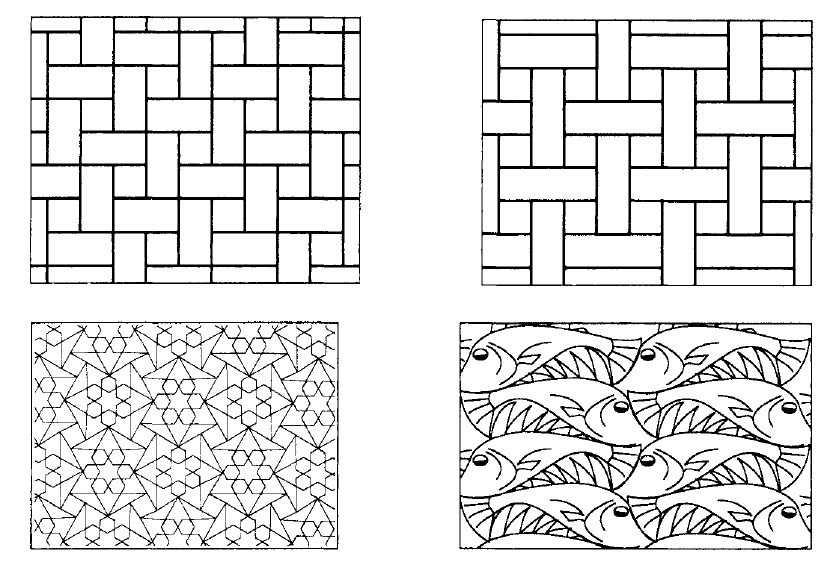
\includegraphics[width=0.95\columnwidth]{artin-algebra-2e-ch06-ex-6.3-patterns.png}

{\tiny 图（Ex.~6.3）：左上 交错矩形、右上 编织、左下 六角星、右下 鱼。}
\end{column}
\begin{column}{0.53\textwidth}
\key{思路}：点群是“作为对称出现的线性部分”全体。先找最大旋转阶 $n$（晶体学限制 $n\le6$），再判断有无镜轴/滑移，最后与 17 种壁纸图案对照。
\key{左上（交错矩形）}：有 $90^\circ,180^\circ,270^\circ$ 旋转中心；交错方向破坏了镜面对称，没有镜轴，故
\[ C_4=\langle r_{90}\rangle,\qquad |C_4|=4, \]
对应表中具纯四重旋转的 $p4$ 类。
\key{右上（编织）}：有 $90^\circ$ 旋转中心，且四个方向都有镜轴（四重中心不在镜轴上），故
\[ D_4=\langle r_{90},s\rangle,\qquad |D_4|=8, \]
对应 $p4g$ 类。
\end{column}
\end{columns}
\end{frame}

\begin{frame}[t]{四、随机复习 14/21：G150 四个壁纸图案的点群（下）}
\scriptsize
\key{左下（六角星与六边形）}：六角星本身带六重对称，星心与六边形中心构成三角格，故有六重旋转中心，并且过它们有镜轴：
\[ D_6=\langle r_{60},s\rangle,\qquad |D_6|=12. \]
晶体学限制（二维版本：$2\cos\theta\in\mathbb Z$）说明不会再大，阶只能是 $1,2,3,4,6$；对应 $p6m$ 类。
\key{右下（鱼）}：没有非平凡旋转（$180^\circ$ 旋转会把鱼身上下翻转，图案不还原），只有一个方向的滑移反射（竖直轴，无纯镜轴），故
\[ D_1=\{1,s\},\qquad |D_1|=2, \]
按 600 dpi 原图判定对应 $pg$ 类（纯镜射命中 $\le0.47$，竖直轴滑移 $0.83$ 与平移上限 $0.84$ 同量级）。
\begin{center}
{\scriptsize
\begin{tabular}{@{}lllll@{}}
\toprule
图案 & 最大旋转阶 & 反向对称 & 点群 & 表 6.6.2 中同类 \\
\midrule
左上 交错矩形 & $4$ & 无 & $C_4$ & $p4$ \\
右上 编织 & $4$ & 镜轴/滑移 & $D_4$ & $p4g$（$p4g$/$p4m$ 细分待核） \\
左下 六角星 & $6$ & 镜轴 & $D_6$ & $p6m$ \\
右下 鱼 & $1$ & 一个方向的滑移（无纯镜轴） & $D_1$ & $pg$ \\
\bottomrule
\end{tabular}}
\end{center}
\key{验算}：对四个图案做旋转/反射的归一化互相关（NCC，全局模板平移搜索；\texttt{checks/R2\_g150\_template\_ncc.py}）：左上、右上在 $90^\circ$ 处 $\approx0.96$、在 $180^\circ$ 处 $\ge0.97$，而在 $60^\circ/120^\circ$ 处 $\le0.16$；右上的四个镜反射 $\ge0.96$，左上仅 $0.77$--$0.79$；右下在所有非平凡旋转处 $\le0.22$，只有单一方向的镜/滑移达到 $0.92$。这些数值与上面的目视判断一致；左下图案线条密集、手绘误差大，NCC 不稳定，改由“六角星 $+$ 三角格”的目视结构定出六重旋转。
\end{frame}

% ==================== Random Review fragment R3 ====================
% ============================================================
% 分片 R3：Random Review k = 15..21（2026-10-26 至 11-01 题单）
%   k=15 G176  正方形作用的忠实性
%   k=16 G23   二面体群中的字归约
%   k=17 LA299 对角二阶矩阵的共轭轨道（2 页）
%   k=18 G154  正方形对称群中的稳定化子（2 页）
%   k=19 G163  S_n 中点稳定化子的陪集（2 页）
%   k=20 G24   二面体群的子群与商群（2 页，保留 (a)(b)(c)）
%   k=21 G167  正四面体的全对称群（2 页）
% 本文件只含 frame 环境，由 wrapper-R3.tex 包裹编译；不含 preamble。
% 所有具体数字均在 checks/R3_checks.py 中独立复算。
% ============================================================

% ---------------------------------------------------------- 15/21 G176
\begin{frame}[t]{四、随机复习 15/21：G176 正方形作用的忠实性}
\label{ex:G176}
\scriptsize
\begin{block}{\footnotesize 题面（\ex{G176}；Artin 2e, Ch.~6, \S11, Ex.~11.4，印刷 p.~192 / PDF p.~204）}
设 $G=D_4$ 是正方形的对称群。$G$ 在四个顶点上的作用是否忠实？$G$ 在两条对角线上的作用是否忠实？
\end{block}
\key{思路}：忠实就是作用同态的核平凡。顶点是四点集、两条对角线是二元集，分别写出核；再用 $|\mathrm{Im}|=|G|/|\ker|$ 交叉核对。

\key{详解}：设 $r$ 是 $90^\circ$ 旋转，$s$ 是关于对角线 $d_1=\{1,3\}$ 的反射，则
\[ G=D_4=\{1,r,r^2,r^3,s,rs,r^2s,r^3s\},\qquad r^4=s^2=1,\quad srs=r^{-1}. \]
\underline{顶点作用忠实}：把顶点按逆时针编号 $1,2,3,4$，则 $r(i)=i+1$，$s$ 固定 $1,3$ 并交换 $2,4$。若 $g\in G$ 固定全部四个顶点，则它固定三个不共线的顶点（例如 $1,2,3$）；平面等距由三个不共线点的像唯一决定，故 $g=1$。所以顶点作用的核是 $\{1\}$，作用忠实。

\underline{对角线作用不忠实}：$G$ 保持“相对顶点对”的集合 $\{d_1,d_2\}$，得同态 $\varphi:G\to S_2$，$\varphi(g)$ 是 $g$ 对两条对角线的置换。逐个算 $8$ 个元素：$\varphi(r)=\varphi(r^3)=\varphi(rs)=\varphi(r^3s)=(d_1d_2)$（这四个元素把 $d_1$ 换成 $d_2$），而 $\varphi(1)=\varphi(r^2)=\varphi(s)=\varphi(r^2s)=1$（$r^2$ 保持两条对角线；$s$ 是关于 $d_1$ 的反射，$r^2s$ 是关于 $d_2$ 的反射，都保持两条对角线）。因此
\[ \ker\varphi=\{1,r^2,s,r^2s\}\cong C_2\times C_2,\qquad |\mathrm{Im}\,\varphi|=8/4=2. \]
核中三个非平凡元都满足 $(r^2)^2=s^2=(r^2s)^2=1$ 且两两交换，故确为 Klein 四元群。

\key{验算}：用置换模型把 $8$ 个元素逐个作用在 $4$ 个顶点和 $2$ 条对角线上（\texttt{checks/R3\_checks.py}）：顶点作用的核阶为 $1$，对角作用的核阶为 $4$、像阶为 $2=8/4$，与上述一致。同一群对不同集合作用，忠实性可以不同，本题就是“四点忠实、两点不忠实”的标准对照。

\key{结论}：对顶点忠实；对两条对角线不忠实，核为 $\{1,r^2,s,r^2s\}\cong C_2\times C_2$。
\end{frame}

% ---------------------------------------------------------- 16/21 G23
\begin{frame}[t]{四、随机复习 16/21：G23 二面体群中的字归约}
\label{ex:G23}
\scriptsize
\begin{block}{\footnotesize 题面（\ex{G23}；Artin 2e, Ch.~6, \S4, Ex.~4.1，印刷 p.~188 / PDF p.~200）}
在二面体群 $D_n=\langle x,y\mid x^n=1,\ y^2=1,\ yx=x^{-1}y\rangle$ 中，把字 $x^2yx^{-1}y^{-1}x^3y^3$ 写成 $x^iy^j$ 的形式。
\end{block}
\key{思路}：用改写规则 $yx^k=x^{-k}y$ 把每个 $y$ 逐次搬到右边，再用 $y^2=1$ 合并；指数 $i$ 最后按 $i\bmod n$ 理解。

\key{详解}：由 $y^2=1$ 得
\[ y^{-1}=y,\qquad y^3=y. \]
改写规则对一切整数 $k$ 成立（$k>0$ 时归纳）：
\[ yx^k=(yx)x^{k-1}=x^{-1}(yx^{k-1})=\cdots=x^{-k}y, \]
$k<0$ 时由 $x^{-k}=(x^k)^{-1}$ 反解得到同一公式；特别取 $k=-1$ 即 $yx^{-1}=xy$。代入原字并逐步归并：
\[
\begin{aligned}
x^2yx^{-1}y^{-1}x^3y^3
&=x^2(yx^{-1})yx^3y\\
&=x^2(xy)yx^3y\\
&=x^3\,(y^2)\,x^3y\\
&=x^6y.
\end{aligned}
\]
即该字 $=x^6y$；标准形（$0\le i<n$）为 $x^{6\bmod n}y$。

\key{验算}：$y$ 在该字中出现 $5$ 次，奇偶性决定结果末尾有 $y$。数值：$n=3$ 时字 $=y$，$n=4$ 时 $=x^2y$，$n=5$ 时 $=xy$，$n=7,8,12$ 时 $=x^6y$；置换模型逐元复核全部吻合（\texttt{checks/R3\_checks.py}）。又 $(x^6y)^2=x^6x^{-6}y^2=1$，故 $x^6y$ 为反射，阶 $2$。
\end{frame}

% ---------------------------------------------------------- 17/21 LA299（上）
\begin{frame}[t]{四、随机复习 17/21：LA299 对角二阶矩阵的共轭轨道（上）}
\label{ex:LA299}
\scriptsize
\begin{block}{\footnotesize 题面（\ex{LA299}；Artin 2e, Ch.~6, \S7, Ex.~7.10，印刷 p.~191 / PDF p.~203）}
(a) 描述 $A=\begin{pmatrix}1&0\\0&2\end{pmatrix}$ 在一般线性群 $GL_n(\mathbb R)$ 共轭作用下的轨道与稳定化子。(b) 把 $A$ 看作 $GL_2(\mathbb F_5)$ 的元素，求其轨道大小。
\end{block}
\starpt{}Source issue：题面 (a) 印作 $GL_n(\mathbb R)$，但矩阵是 $2\times2$；未给嵌入约定时 $n\neq2$ 的作用无定义，故按 (b) 与题目原意取 $n=2$。

\key{思路}：共轭作用 $P\cdot A=PAP^{-1}$，稳定化子即中心化子。$A$ 的特征值 $1\neq2$ 互异，故与之交换的矩阵必为对角阵；轨道由相似不变量与轨道--稳定化子刻画。

\key{详解（稳定化子）}：设 $P=\begin{pmatrix}p&q\\r&s\end{pmatrix}$，直接计算
\[ PA=\begin{pmatrix}p&2q\\r&2s\end{pmatrix},\qquad AP=\begin{pmatrix}p&q\\2r&2s\end{pmatrix}. \]
由 $PA=AP$ 得 $q=2q$、$r=2r$，即 $q=r=0$；反之任意对角可逆矩阵都与 $A$ 交换。因此
\[ Z_{GL_2(\mathbb R)}(A)=\left\{\begin{pmatrix}p&0\\0&s\end{pmatrix}:p,s\in\mathbb R^\times\right\}. \]
\key{详解（轨道）}：相似矩阵有相同的迹与行列式，故 $\operatorname{Orb}(A)\subseteq\{B\in M_2(\mathbb R):\operatorname{tr}B=3,\ \det B=2\}$。反方向：若 $\operatorname{tr}B=3$、$\det B=2$，则特征多项式
\[ \chi_B(\lambda)=\lambda^2-3\lambda+2=(\lambda-1)(\lambda-2), \]
两特征根 $1\neq2$ 为实数，故 $B$ 在 $\mathbb R$ 上可对角化：存在 $Q\in GL_2(\mathbb R)$ 使 $B=Q\operatorname{diag}(1,2)Q^{-1}=QAQ^{-1}$。于是
\[ \operatorname{Orb}(A)=\{B\in M_2(\mathbb R):\operatorname{tr}B=3,\ \det B=2\},\qquad \dim\operatorname{Orb}(A)=2. \]
\end{frame}

% ---------------------------------------------------------- 17/21 LA299（下）
\begin{frame}[t]{四、随机复习 17/21：LA299 对角二阶矩阵的共轭轨道（下）}
\scriptsize
\key{(b) 详解}：$|GL_2(\mathbb F_5)|=(5^2-1)(5^2-5)=24\cdot20=480$。同一中心化子计算在 $\mathbb F_5$ 上给出
\[ Z_{GL_2(\mathbb F_5)}(A)=\left\{\begin{pmatrix}p&0\\0&s\end{pmatrix}:p,s\in\mathbb F_5^\times\right\},\qquad |Z|=4^2=16. \]
由轨道--稳定化子，
\[ |\operatorname{Orb}(A)|=\frac{|GL_2(\mathbb F_5)|}{|Z|}=\frac{480}{16}=30. \]
\key{验算 1（独立计数）}：直接数 $\mathbb F_5$ 上满足 $\operatorname{tr}B=3$、$\det B=2$ 的矩阵 $B=\begin{pmatrix}a&b\\c&d\end{pmatrix}$。由 $d=3-a$ 得 $bc=ad-2=:t$。$t=0$ 时 $(b,c)$ 有 $5+5-1=9$ 对；$t\neq0$ 时对每个 $b\neq0$ 有唯一 $c=t/b$，共 $4$ 对。按 $a$ 分类：
\[
\begin{aligned}
a=1,2&:\quad d=2,1,\quad t=0\ \Rightarrow\ 9+9;\\
a=0,3,4&:\quad t=-2\equiv3\neq0\ \Rightarrow\ 4+4+4.
\end{aligned}
\]
合计 $9+9+4+4+4=30$，与 $480/16=30$ 一致；且这 $30$ 个矩阵的特征多项式都是 $(\lambda-1)(\lambda-2)$，在 $\mathbb F_5$ 上互异，故互相对角化并相似，恰是轨道。

\key{验算 2（群枚举）}：枚举全部 $480$ 个 $GL_2(\mathbb F_5)$ 元素共轭 $A$，得到 $30$ 个不同矩阵；枚举中心化子恰 $16$ 个；轨道恰等于 $\{\operatorname{tr}=3,\det=2\}$（也是 $30$ 个）。见 \texttt{checks/R3\_checks.py}。

\starpt{}两种情形对照：$\mathbb R$ 上轨道是“迹 $3$、行列式 $2$”的二维连续族，稳定化子无限；$\mathbb F_5$ 上同一描述只剩 $30$ 个矩阵，用有限群计数必须走轨道--稳定化子。两种情形下“特征值互异”都保证 $A$ 的相似类被特征多项式唯一确定。
\end{frame}

% ---------------------------------------------------------- 18/21 G154（上）
\begin{frame}[t]{四、随机复习 18/21：G154 正方形对称群中的稳定化子（上）}
\label{ex:G154}
\scriptsize
\begin{block}{\footnotesize 题面（\ex{G154}；Artin 2e, Ch.~6, \S7, Ex.~7.1，印刷 p.~190 / PDF p.~202）}
设 $G=D_4$ 是正方形的对称群。(a) 一个顶点的稳定化子是什么？一条边的稳定化子是什么？(b) $G$ 作用在由两条对角线组成的二元集合上，一条对角线的稳定化子是什么？
\end{block}
\key{思路}：先用轨道--稳定化子 $|G_x|\cdot|\operatorname{Orb}(x)|=|G|=8$ 定出阶，再按几何条件把元素写全：固定一个顶点 $=$ 关于过该顶点的对角线的反射；保持一条边（集合意义）$=$ 关于该边垂直平分线的反射。

\key{详解 (a)}：设 $r$ 是 $90^\circ$ 旋转。四个顶点在同一轨道上（$r$ 循环移动它们），故 $|G_v|=8/4=2$。取顶点 $1$，设 $d_1=\{1,3\}$ 是过 $1$ 的对角线，$s$ 是关于 $d_1$ 的反射，则 $s$ 固定顶点 $1$。顶点 $1$ 的稳定化子含 $1,s$ 且阶为 $2$，故
\[ G_1=\{1,s\}\cong C_2. \]
四条边也在同一轨道上（$r$ 循环移动它们），故 $|G_e|=8/4=2$。取边 $e=\{1,2\}$：关于 $e$ 的垂直平分线的反射交换 $1,2$、保持 $e$ 不变，它就是 $rs$；恒等也保持 $e$。于是
\[ G_{\{1,2\}}=\{1,rs\}\cong C_2. \]
\starpt{}注意“边的稳定化子”是集合意义（$G$ 作用在边集合上）。若要求逐点固定一条边的两个端点，则只有恒等：固定顶点 $1$ 的对称只有 $1,s$，而 $s$ 把边 $\{1,2\}$ 的两端点互换，故逐点稳定化子平凡。

\key{验算}：用 $8$ 个元素在顶点上的置换模型逐个检验（\texttt{checks/R3\_checks.py}）：顶点 $1$ 的稳定化子 $\{1,s\}$，边 $\{1,2\}$ 的稳定化子 $\{1,rs\}$，阶均为 $2$，与轨道大小 $4$ 及 $|G|=8$ 吻合。
\end{frame}

% ---------------------------------------------------------- 18/21 G154（下）
\begin{frame}[t]{四、随机复习 18/21：G154 正方形对称群中的稳定化子（下）}
\scriptsize
\key{详解 (b)}：两条对角线 $d_1=\{1,3\}$、$d_2=\{2,4\}$ 组成二元集，$G$ 保持它；$r$ 把 $d_1$ 送到 $d_2$，故作用传递，轨道大小为 $2$，于是 $|G_{d_1}|=8/2=4$。显式地
\[ G_{d_1}=\{1,r^2,s,r^2s\}=\{1,r^2\}\cdot\{1,s\}\cong C_2\times C_2. \]
逐元核对：$s$（关于 $d_1$ 的反射）固定 $d_1$ 上的每个点；$r^2$ 是 $180^\circ$ 旋转，交换 $d_1$ 的两个端点、保持 $d_1$ 集合不变；$r^2s$ 是关于 $d_2$ 的反射，同样交换 $d_1$ 的两个端点。而 $r,rs$ 把 $d_1$ 送到 $d_2$。所以四个元素都保持 $d_1$，阶为 $4$，恰是稳定化子。

\key{验算}：同一个置换模型（\texttt{checks/R3\_checks.py}）给出：对角线 $d_1$ 的稳定化子恰为 $\{1,r^2,s,r^2s\}$，阶 $4$；$d_2$ 的稳定化子相同；三个非平凡元均二阶且两两交换，故 $\cong C_2\times C_2$。与 (a) 合起来：顶点、边、对角线的轨道大小分别为 $4,4,2$，稳定化子阶分别为 $2,2,4$，乘积都等于 $|G|=8$。

\key{结构说明}：$G_{d_1}=G_{d_2}=\ker\bigl(G\to S_2\bigr)$，即 $G$ 在两条对角线上作用的核。两个稳定化子都等于核，因为它们的阶都是 $4$，而核是二者的交、阶也是 $8/2=4$。这与 k=15 的 G176 结论一致：该二点作用的核正是 $\{1,r^2,s,r^2s\}$。

\key{易错}：不要混淆“稳定化子”与“固定某点/某边的元素个数”。顶点稳定化子固定该顶点（点意义），边与对角线稳定化子保持该子集（集合意义）；边稳定化子中唯一的非平凡元会把边的两个端点互换。
\end{frame}

% ---------------------------------------------------------- 19/21 G163（上）
\begin{frame}[t]{四、随机复习 19/21：G163 $S_n$ 中点稳定化子的陪集（上）}
\label{ex:G163}
\scriptsize
\begin{block}{\footnotesize 题面（\ex{G163}；Artin 2e, Ch.~6, \S8, Ex.~8.4，印刷 p.~191 / PDF p.~203）}
设 $H$ 是 $G=S_n$ 在指标集 $\{1,\dots,n\}$ 上作用时下标 $1$ 的稳定化子。描述 $H$ 在 $G$ 中的左陪集，并描述此情形下的映射 (6.8.4)。
\end{block}
\key{思路}：左陪集 $\sigma H$ 由“$\sigma$ 把 $1$ 送到哪个指标”决定；用对换 $\tau_i=(1\ i)$ 作为代表元，把 $n$ 个左陪集与 $1,\dots,n$ 一一对应。映射 (6.8.4) 就是陪集到轨道点的双射 $\sigma H\mapsto\sigma(1)$。

\key{详解}：$H=\{\sigma\in S_n:\sigma(1)=1\}$ 中的置换可任意置换 $2,\dots,n$，故
\[ H\cong S_{n-1},\qquad |H|=(n-1)!. \]
由轨道--稳定化子，$|\operatorname{Orb}(1)|=|S_n|/|H|=n!/(n-1)!=n$，即作用传递、$1$ 的轨道是全部指标。
关键是算出陪集：设 $\sigma(1)=i$，取 $\tau_i=(1\ i)$（约定 $\tau_1=1$）。注意到
\[ (\tau_i\sigma)(1)=\tau_i\bigl(\sigma(1)\bigr)=\tau_i(i)=1, \]
故 $h:=\tau_i\sigma\in H$，从而 $\sigma=\tau_i h$（用 $\tau_i^2=1$），即 $\sigma H=\tau_i H$。反过来，若 $\sigma H=\tau_i H$，则 $\sigma=\tau_i h$（$h\in H$），于是
\[ \sigma(1)=\tau_i\bigl(h(1)\bigr)=\tau_i(1)=i. \]
两句话合起来就是
\[ \sigma H=\tau_{\sigma(1)}H. \]
因此 $S_n/H=\{\tau_iH:1\le i\le n\}$，且这些陪集两两不同：若 $\tau_iH=\tau_jH$，则 $i=\tau_i(1)$ 与 $j$ 相等（由上式）。共 $n$ 个左陪集，每个大小为 $|H|=(n-1)!$。
\end{frame}

% ---------------------------------------------------------- 19/21 G163（下）
\begin{frame}[t]{四、随机复习 19/21：G163 $S_n$ 中点稳定化子的陪集（下）}
\scriptsize
\key{映射 (6.8.4)}：Artin 的公式把左陪集与轨道点对应，本题取轨道点 $x_0=1$：
\[ \Phi:S_n/H\longrightarrow\{1,\dots,n\},\qquad \sigma H\longmapsto \sigma(1). \]
\key{良定义与双射}：若 $\sigma H=\sigma'H$，则 $\sigma'=\sigma h$（$h\in H$），故 $\sigma'(1)=\sigma(h(1))=\sigma(1)$，$\Phi$ 良定义。单射：若 $\sigma(1)=\sigma'(1)=i$，则 $\tau_i\sigma,\tau_i\sigma'\in H$，故 $\sigma H=\tau_iH$ 且 $\sigma'H=\tau_iH$，即 $\sigma H=\sigma'H$。满射：$\Phi(\tau_iH)=i$，$i=1,\dots,n$ 全部取到。所以 $\Phi$ 是双射。

\key{具体小例（$n=3$）}：$H=\{1,(23)\}$，三个左陪集为
\begin{center}
{\scriptsize
\begin{tabular}{@{}lll@{}}
\toprule
代表元 & 左陪集 & $\Phi$ 的值\\
\midrule
$\tau_1=1$ & $H=\{1,(23)\}$ & $1$\\
$\tau_2=(12)$ & $(12)H=\{(12),(123)\}$ & $2$\\
$\tau_3=(13)$ & $(13)H=\{(13),(132)\}$ & $3$\\
\bottomrule
\end{tabular}}
\end{center}
逐项核：$(12)(23)=(123)$，$(123)(1)=2$；$(13)(23)=(132)$，$(132)(1)=3$。正好一一对应。

\key{验算}：对 $n=2,3,4,5,6$ 枚举 $S_n$ 全部置换（\texttt{checks/R3\_checks.py}）：左陪集数都等于 $n$，每个 $\sigma$ 都满足 $\sigma H=\tau_{\sigma(1)}H$，且 $\Phi$ 是双射，与 $|S_n|/|H|=n$ 一致。

\starpt{}注意这里必须是左陪集：对右陪集 $H\sigma$，结论变为由 $\sigma^{-1}(1)$ 决定。因为 $\sigma H$ 中元素形如 $\sigma h$，$(\sigma h)(1)=\sigma(h(1))$ 与 $\sigma(1)$ 无关；而 $H\sigma=\{\sigma h\}$ 的写法下右乘会把 $1$ 的像打乱，改由 $\sigma^{-1}(1)$ 分类。
\end{frame}

% ---------------------------------------------------------- 20/21 G24（上）
\begin{frame}[t]{四、随机复习 20/21：G24 二面体群的子群与商群（上）}
\label{ex:G24}
\scriptsize
\begin{block}{\footnotesize 题面（\ex{G24}；Artin 2e, Ch.~6, \S4, Ex.~4.2，印刷 p.~188 / PDF p.~200）}
设 $D_n=\langle x,y\mid x^n=1,\ y^2=1,\ yxy=x^{-1}\rangle$，$|D_n|=2n$。(a) 列出 $D_4$ 的全部子群，并判定哪些正规。(b) 列出 $D_{15}$ 的全部真正规子群 $N$，并确定 $D_{15}/N$。(c) 列出 $D_6$ 中不含 $x^3$ 的子群。
\end{block}
\key{思路}：按“旋转部分”$H\cap\langle x\rangle$ 分类。$H\le D_n$ 要么含于 $\langle x\rangle$（循环群子群由 $d\mid n$ 给出 $\langle x^d\rangle$），要么含反射，此时 $H=\langle x^d,x^ky\rangle$，$d\mid n$，$k\bmod d$ 决定子群，阶为 $2n/d$。正规性用“指数 $2$ 的子群正规”与共轭公式 $x^j(x^ky)x^{-j}=x^{k+2j}y$。

\key{(a) 详解}：$D_4=\langle x,y\rangle$，$x^4=y^2=1$。按 $d\mid4$ 分类：
\begin{center}
{\scriptsize
\begin{tabular}{@{}cll@{}}
\toprule
阶 & 子群 & 个数\\
\midrule
$1$ & $\{1\}$ & $1$\\
$2$ & $\langle x^2\rangle$（中心）；$\langle y\rangle,\langle xy\rangle,\langle x^2y\rangle,\langle x^3y\rangle$ & $5$\\
$4$ & $\langle x\rangle$；$\langle x^2,y\rangle=\{1,x^2,y,x^2y\}$；$\langle x^2,xy\rangle=\{1,x^2,xy,x^3y\}$ & $3$\\
$8$ & $D_4$ & $1$\\
\bottomrule
\end{tabular}}
\end{center}
穷尽性：若 $H\le\langle x\rangle$，则 $H$ 是 $\{1\},\langle x^2\rangle,\langle x\rangle$ 之一；若 $H\not\le\langle x\rangle$，取 $x^ky\in H$，由 $H\cap\langle x\rangle=\langle x^d\rangle$（$d\mid4$）得 $H=\langle x^d,x^ky\rangle$，其中 $k$ 只由 $k\bmod d$ 决定：$d=4$ 给 $4$ 个反射子群，$d=2$ 给 $2$ 个 Klein 四元群，$d=1$ 给 $D_4$。合计 $1+5+3+1=10$ 个子群。
正规子群共 $6$ 个：$\{1\}$；$\langle x^2\rangle$（中心，$x^2$ 与 $x,y$ 都交换）；$\langle x\rangle,\langle x^2,y\rangle,\langle x^2,xy\rangle$（后三者指数 $2$）；$D_4$。四个反射子群 $\langle x^ky\rangle$ 不正规，因为
\[ x\,(x^ky)\,x^{-1}=x^{k+1}yx^{-1}=x^{k+2}y, \]
其中用了 $yx^{-1}=xy$；而 $\langle x^ky\rangle\neq\langle x^{k+2}y\rangle$（$k$ 与 $k+2$ 奇偶性不同），故反射子群在共轭下改变。
\end{frame}

% ---------------------------------------------------------- 20/21 G24（下）
\begin{frame}[t]{四、随机复习 20/21：G24 二面体群的子群与商群（下）}
\scriptsize
\key{(b) 详解}：$n=15$ 为奇数。$\langle x\rangle\cong C_{15}$ 的每个阶的子群唯一，故 $\langle x^d\rangle$ 是 $\langle x\rangle$ 的特征子群，从而是 $D_{15}$ 的正规子群。这给出 $4$ 个真正规子群：$\{1\}$、$\langle x^5\rangle$（阶 $3$）、$\langle x^3\rangle$（阶 $5$）、$\langle x\rangle$（阶 $15$）。
没有其他真正规子群：若 $N$ 含反射 $x^ky$，由共轭公式及 $\gcd(2,15)=1$ 知 $N$ 含全部 $15$ 个反射；取两个不同反射，其积为某 $1\neq x^m$，共轭得 $\langle x\rangle\le N$，故 $N=D_{15}$。商群如下：
\begin{center}
{\scriptsize
\begin{tabular}{@{}lllll@{}}
\toprule
$N$ & $|N|$ & $|D_{15}/N|$ & $D_{15}/N$ & 识别依据\\
\midrule
$\{1\}$ & $1$ & $30$ & $D_{15}$ & 自身\\
$\langle x^5\rangle$ & $3$ & $10$ & $D_5$ & $\bar x$ 阶 $15/3=5$，$\bar y\bar x\bar y=\bar x^{-1}$\\
$\langle x^3\rangle$ & $5$ & $6$ & $D_3\cong S_3$ & $\bar x$ 阶 $15/5=3$，同上\\
$\langle x\rangle$ & $15$ & $2$ & $C_2$ & 只剩 $\bar y\neq1$\\
\bottomrule
\end{tabular}}
\end{center}
\key{(c) 详解}：$D_6$（阶 $12$）的子群有旋转部分 $\langle x^d\rangle$，$d\mid6$。子群含 $x^3$ 当且仅当旋转部分含 $x^3$，当且仅当 $d\mid3$，故不含 $x^3$ 的只有 $d=6$ 与 $d=2$ 两族：
\begin{center}
{\scriptsize
\begin{tabular}{@{}clll@{}}
\toprule
$d$ & 子群 & 阶 & 个数\\
\midrule
$6$ & $\{1\}$；$\langle x^ky\rangle=\{1,x^ky\}$，$k=0,\dots,5$ & $1,2$ & $1+6$\\
$2$ & $\langle x^2\rangle=\{1,x^2,x^4\}$；$\langle x^2,y\rangle,\langle x^2,xy\rangle$ & $3,6$ & $1+2$\\
\bottomrule
\end{tabular}}
\end{center}
共 $10$ 个；两个 $6$ 阶子群（均不含 $x^3$）为 $\langle x^2,y\rangle$ 与 $\langle x^2,xy\rangle$。

\key{验算}：置换模型枚举（\texttt{checks/R3\_checks.py}）：$D_4$ 共 $10$ 个（正规 $6$），$D_{15}$ 共 $28$ 个（真正规 $4$），$D_6$ 共 $16$ 个（不含 $x^3$ 的恰 $10$）。
\end{frame}

% ---------------------------------------------------------- 21/21 G167（上）
\begin{frame}[t]{四、随机复习 21/21：G167 正四面体的全对称群（上）}
\label{ex:G167}
\scriptsize
\begin{block}{\footnotesize 题面（\ex{G167}；Artin 2e, Ch.~6, \S9, Ex.~9.4，印刷 p.~191 / PDF p.~203）}
确定正四面体的全对称群 $T'$，即包括改变定向的对称在内的全部对称构成的群。
\end{block}
\key{思路}：$T'$ 置换 $4$ 个顶点，得同态 $\rho:T'\to S_4$。单射：等距由 $4$ 个仿射无关点的像唯一决定；满射：正四面体任意两顶点距离相等，故任一顶点置换都保持距离、唯一延拓为空间等距。于是 $T'\cong S_4$。

\key{详解}：设顶点为 $v_1,\dots,v_4$，它们仿射无关（不共面）。每个 $g\in T'$ 置换顶点集，定义 $\rho(g)\in S_4$ 为对应的顶点置换。

\underline{单射}：若 $\rho(g)=1$，则 $g$ 固定 $v_1,\dots,v_4$ 四个点；$\mathbb R^3$ 的等距由它在 $4$ 个仿射无关点上的像唯一决定，故 $g=1$，即 $\ker\rho=\{1\}$。

\underline{满射}：正四面体任意一对相异顶点的距离都等于棱长 $a$，故对任意 $\pi\in S_4$ 有 $|v_{\pi(i)}-v_{\pi(j)}|=|v_i-v_j|$，即 $\pi$ 是四点集到自身的距离保持双射。取唯一仿射映射 $A$ 使 $A(v_i)=v_{\pi(i)}$（$v_1,\dots,v_4$ 仿射无关保证存在且唯一）。$A$ 的线性部分把 $v_2-v_1,v_3-v_1,v_4-v_1$ 送到 $v_{\pi(2)}-v_{\pi(1)},\dots$；而任意两向量的内积由三点间距离决定：
\[ \langle v_i-v_1,v_j-v_1\rangle=\frac{|v_i-v_1|^2+|v_j-v_1|^2-|v_i-v_j|^2}{2}, \]
且右端在 $\pi$ 下不变。因此 $A$ 的线性部分保持内积、是正交变换，$A$ 是 $\mathbb R^3$ 的等距，并把正四面体送到自身，即 $A\in T'$ 且 $\rho(A)=\pi$。
所以 $\rho$ 既是单射又是满射，$T'\cong S_4$，$|T'|=4!=24$。
\end{frame}

% ---------------------------------------------------------- 21/21 G167（下）
\begin{frame}[t]{四、随机复习 21/21：G167 正四面体的全对称群（下）}
\scriptsize
\key{旋转子群是 $A_4$}：对 $g\in T'$，$\det g$ 的符号等于顶点置换 $\rho(g)$ 的奇偶性，故保向元素恰对应偶置换：
\[ T=\{g\in T':\det g=1\}\cong A_4,\qquad |T|=12, \]
而反向对称有 $12$ 个。

\key{旋转的具体计数}：$A_4$ 的 $12$ 个元素按阶分为 $1+8+3$。几何上：$1$ 个恒等；$8$ 个 $3$ 阶旋转绕“顶点--对面中心”轴，共 $4$ 条轴，每条轴有 $\pm120^\circ$ 两个非平凡旋转；$3$ 个 $2$ 阶旋转绕三对对棱中点连线，各一个 $180^\circ$ 旋转。$1+8+3=12$。

\key{反向对称的具体形状}：$12$ 个奇置换中，$6$ 个对换对应 $6$ 个镜面反射（镜面过一条棱与对棱中点，正四面体共有 $6$ 条棱）；$6$ 个 $4$-循环对应 $6$ 个反旋转（先绕对棱中点连线转 $90^\circ$ 再关于垂直平面反射，三对对棱中点连线各给两个）。

\key{验算}：取顶点 $(1,1,1),(1,-1,-1),(-1,1,-1),(-1,-1,1)$，枚举 $3!\cdot2^3=48$ 个符号置换矩阵（\texttt{checks/R3\_checks.py}）：把顶点集送到自身的恰 $24$ 个，它们给出的顶点置换两两不同且覆盖 $S_4$ 的全部 $24$ 个元素；$\det=+1$ 的 $12$ 个与偶置换一致，$\det=-1$ 的 $12$ 个与奇置换一致，旋转按阶恰为 $1+8+3$。

\starpt{}易错：只数保向对称会得到 $12$ 阶的 $A_4$；题目 $T'$ 含反向对称，故答案是 $24$ 阶的 $S_4$。顶点置换模型自动包含反向对称，不会漏。
\end{frame}

% ==================== Systematic Progress fragment S1 ====================
% ============================================================
% frag-S1.tex : Systematic Progress k = 1..7
% G227, G228, G229, LA307, G230, G231, G232 (Artin 2e, Ch. 7, §7--§8)
% Wrapped by wrapper-S1.tex; contains frames only.
% ============================================================

% ---------------------------------------------------------- S1/21 G227
\begin{frame}[t]{五、系统推进 1/21：G227 四个旋转群的 Sylow 2-子群（上）}
\label{ex:G227}
\scriptsize
\begin{block}{\footnotesize 题面（\ex{G227}；Artin 2e, Ch.~7, §7, Ex.~7.5，印刷 p.~224 / PDF p.~236）}
求下列各群的 Sylow 2-子群：\textbf{(a)} $D_{10}$；\textbf{(b)} $T$；\textbf{(c)} $O$；\textbf{(d)} $I$。
\end{block}
\key{思路}：Sylow 2-子群的阶取 $|G|$ 的 2-部分；先代入标准同构 $T\cong A_4$、$O\cong S_4$、$I\cong A_5$（$T,O,I$ 分别为正四面体、正八面体、正二十面体的旋转群）与 Artin 约定 $|D_{10}|=20$，再按“无 4 阶元则 $\cong V_4$，有 4 阶元则 $\cong D_4$”显式构造。

\key{(a) $D_{10}$}：$D_{10}=\langle r,s\mid r^{10}=s^2=1,\ srs=r^{-1}\rangle$，$|D_{10}|=20=2^2\cdot5$。$r^k$ 的阶整除 $10$，$r^ks$ 的阶为 $2$，故 $D_{10}$ 无 4 阶元，其 Sylow 2-子群 $\cong V_4$：
\[ P=\langle r^5,s\rangle=\{1,\ r^5,\ s,\ r^5s\},\qquad (r^5)^2=s^2=(r^5s)^2=1. \]
由 $n_2\mid5$、$n_2\equiv1\pmod2$（Sylow III）得 $n_2\in\{1,5\}$；而 $rPr^{-1}=\langle r^5,r^2s\rangle\ne P$，故 $n_2=5$，五个 Sylow 2-子群为
\[ P_k=\langle r^5,\,r^{2k}s\rangle,\qquad k=0,1,2,3,4. \]

\key{(b) $T\cong A_4$}：$|A_4|=12=2^2\cdot3$，Sylow 2-子群阶为 4。$A_4$ 的元素为 $1$、$3$ 个双换位、$8$ 个三循环，无 4 阶元，故 Sylow 2-子群必为
\[ V_4=\{1,\ (12)(34),\ (13)(24),\ (14)(23)\}. \]
它由 $1$ 与三个双换位组成，而三个双换位在 $A_4$ 中构成一个共轭类，故 $V_4\triangleleft A_4$，$n_2=1$。几何上这是三条对棱中点轴上的 $180^\circ$ 旋转连同恒等。
\end{frame}

% ---------------------------------------------------------- S1/21 G227
\begin{frame}[t]{五、系统推进 1/21：G227 四个旋转群的 Sylow 2-子群（下）}
\scriptsize
\key{(c) $O\cong S_4$}：$|S_4|=24=2^3\cdot3$，Sylow 2-子群阶为 8。取
\[ P=\langle(1234),(13)\rangle,\qquad (13)(1234)(13)=(1432)=(1234)^{-1}, \]
故 $P$ 由 4 阶元与其反演生成，$P\cong D_4$，$|P|=8$。不同 Sylow 2-子群对应 $\{1,2,3,4\}$ 的三种二划分
\[ \{12\,|\,34\},\qquad\{13\,|\,24\},\qquad\{14\,|\,23\}, \]
每一种划分的稳定化子 $\cong D_4$、阶 $24/3=8$，故 $n_2\ge3$；又 $n_2\mid3$、$n_2\equiv1\pmod2$，得 $n_2=3$。几何上这是三对相对面：绕面心轴 $90^\circ$ 的 $C_4$ 加上 4 条水平二重轴。

\key{(d) $I\cong A_5$}：$|A_5|=60=2^2\cdot15$，Sylow 2-子群阶为 4。$A_5$ 的轮换型只有 $1$、$2^2$、$3$、$5$，无 4 阶元，故 Sylow 2-子群 $\cong V_4$，由 $1$ 与三个双换位组成。双换位共 $15$ 个，每个 $V_4$ 恰含 3 个，故
\[ n_2=\frac{15}{3}=5. \]
显式地，对每个 $i\in\{1,\dots,5\}$，取 $V_i=\{1\}\cup\{\text{固定 }i\text{ 的三个双换位}\}$；$V_i$ 是固定 $i$ 的那个 $A_4$ 的 Sylow 2-子群（每个对合都含于某个 Sylow 2-子群，故 $15$ 个对合被 5 个 $V_4$ 均分）。

\key{验算}：$n_2$ 依次为 $(5,1,3,5)$。$D_{10}$：五个 $V_4$ 都含中心元 $r^5$，各含 2 个反射，共覆盖 $5\times2=10$ 个反射，故全部对合为 $1+10=11$ 个，与阶分布 $1,11,4,4$（$1,2,5,10$ 阶元个数）一致。$A_4$：3 个双换位恰为一个 $V_4$ 的全部非单位元。$S_4$：每个 $D_4$ 含 2 个四循环，$3\times2=6$ 恰为全部四循环数。$A_5$：$5\times3=15$ 恰为全部双换位数。
\end{frame}

% ---------------------------------------------------------- S2/21 G228
\begin{frame}[t]{五、系统推进 2/21：G228 $S_7$ 中 21 阶非交换子群}
\label{ex:G228}
\scriptsize
\begin{block}{\footnotesize 题面（\ex{G228}；Artin 2e, Ch.~7, §7, Ex.~7.6，印刷 p.~224 / PDF p.~236）}
在 $S_7$ 中给出一个 21 阶的非交换子群。
\end{block}
\key{思路}：在 $\mathbb F_7$ 上取仿射变换 $t\mapsto at+b$，乘法部分取 $\mathbb F_7^\times$ 的 3 阶子群 $\langle2\rangle=\{1,2,4\}$，得到 $C_7\rtimes C_3$；它忠实作用在 7 个点上，从而嵌入 $S_7$。

\key{详解}：令 $a:t\mapsto t+1$，$b:t\mapsto2t$（在 $\mathbb F_7$ 上）。$a$ 的阶为 7；由 $2^3=8\equiv1$、$2\ne1$，$b$ 的阶为 3。由 $2\cdot4=8\equiv1$ 得 $b^{-1}:t\mapsto4t$，于是
\[ bab^{-1}(t)=b\bigl(a(4t)\bigr)=b(4t+1)=8t+2\equiv t+2=a^2(t),\qquad\text{即 }bab^{-1}=a^2. \]
因此 $ba\ne ab$（否则 $a^2=a$），$\langle a,b\rangle$ 非交换；又 $\langle a\rangle\cap\langle b\rangle=1$（阶互素），故
\[ |\langle a,b\rangle|=7\cdot3=21. \]
把 $\mathbb F_7$ 的点 $t$ 写成文字 $t+1\in\{1,\dots,7\}$，则
\[ a=(1\,2\,3\,4\,5\,6\,7),\qquad b=(2\,3\,5)(4\,7\,6), \]
故 $G=\langle(1234567),(235)(476)\rangle\le S_7$ 即为所求。

\key{验算}：用 $bab^{-1}=a^2$ 得 $ba^ib^{-1}=a^{2i}$，故
\[ (a^ib)^2=a^{3i}b^2,\qquad (a^ib)^3=a^{3i}b^2a^ib=a^{3i}a^{4i}b^3=a^{7i}=1, \]
即每个 $a^ib$ 的阶为 3，且 $(a^ib)^{-1}=(a^ib)^2=a^{3i}b^2$。21 个元素为：$1$；$a^i\ (i=1,\dots,6)$ 共 6 个 7 阶元；$a^ib,\ a^ib^2$ 共 14 个 3 阶元。故 $n_7=1$、$n_3=7$，且 $1+6+14=21$。
\end{frame}

% ---------------------------------------------------------- S3/21 G229
\begin{frame}[t]{五、系统推进 3/21：G229 $p$ 只整除群阶一次时的 Sylow 轨道}
\label{ex:G229}
\scriptsize
\begin{block}{\footnotesize 题面（\ex{G229}；Artin 2e, Ch.~7, §7, Ex.~7.7，印刷 p.~224 / PDF p.~236）}
设 $|G|=pm$ 且 $p\nmid m$；$H$ 是一个 Sylow $p$-子群，$S$ 为全部 Sylow $p$-子群之集。解释 $S$ 在 $H$ 共轭作用下的轨道分解。
\end{block}
\key{思路}：$H$ 共轭作用在 $S$ 上，轨道长整除 $|H|=p$，故只为 $1$ 或 $p$；再证明唯一的不动点是 $H$ 本身。

\key{详解}：作用为 $H\times S\to S$，$(h,K)\mapsto hKh^{-1}$。由轨道–稳定化子定理，$K$ 的轨道长 $=[H:\operatorname{Stab}_H(K)]\in\{1,p\}$。$H$ 固定自身：$hHh^{-1}=H$。若 $K\in S$ 也被整个 $H$ 固定，则 $H\le N_G(K)$，于是 $HK$ 是 $G$ 的子群；因 $|H|=p$ 为素数，$H\ne K$ 时 $H\cap K=1$，故
\[ |HK|=\frac{|H|\,|K|}{|H\cap K|}=p^2,\qquad\text{但 }HK\le G\ \Longrightarrow\ p^2\mid|G|=pm, \]
与 $p\nmid m$ 矛盾。所以 $K=H$，即 $S$ 中唯一的 1 元轨道是 $\{H\}$，其余轨道长均为 $p$：
\[ S=\{H\}\sqcup\{\text{若干 }p\text{ 元轨道}\},\qquad |S|=1+p\,r\equiv1\pmod p. \]
这正是 Sylow III 同余 $n_p\equiv1\pmod p$ 的轨道证明。

\key{验算 1（$A_4$，$p=3$）}：$|A_4|=3\cdot4$，$S=\{\langle(123)\rangle,\langle(124)\rangle,\langle(134)\rangle,\langle(234)\rangle\}$。取 $H=\langle(123)\rangle$，则 $H$ 固定自身，且
\[ (123)\langle(124)\rangle(123)^{-1}=\langle(234)\rangle,\qquad (132)\langle(124)\rangle(132)^{-1}=\langle(134)\rangle, \]
故分解为 $4=1+3$（$r=1$），不动点唯一。

\key{验算 2（$S_5$，$p=5$）}：$|S_5|=5\cdot24$，$n_5=6$，$H=\langle(12345)\rangle$ 的轨道分解为 $6=1+5$（$r=1$）。
\end{frame}

% ---------------------------------------------------------- S4/21 LA307
\begin{frame}[t]{五、系统推进 4/21：LA307 $GL_n(\mathbb F_p)$ 的 Sylow $p$-子群（上）}
\label{ex:LA307}
\scriptsize
\begin{block}{\footnotesize 题面（\ex{LA307}；Artin 2e, Ch.~7, §7, Ex.~7.8，印刷 p.~224 / PDF p.~236）}
计算 $|GL_n(\mathbb F_p)|$；求出一个 Sylow $p$-子群，并确定 Sylow $p$-子群的个数。
\end{block}
\key{思路}：数有序基给出 $|GL_n|$，其 $p$-部分为 $p^{n(n-1)/2}$；上单位三角群 $U$ 恰好达到这个阶，故为 Sylow $p$-子群；再用正规化子 $N_G(U)=B$（可逆上三角群）算 $n_p$。

\key{详解 (i)：$|GL_n(\mathbb F_p)|$}：第 $i+1$ 个基向量（$i=0,\dots,n-1$）不能落在前 $i$ 个向量张成的 $\mathbb F_p^i$ 中，有 $p^n-p^i$ 种选法，故
\[ |GL_n(\mathbb F_p)|=\prod_{i=0}^{n-1}(p^n-p^i)=p^{\frac{n(n-1)}2}\prod_{k=1}^{n}(p^k-1), \]
第二步用了 $p^n-p^i=p^i(p^{n-i}-1)$ 与 $\sum_{i=0}^{n-1}i=\frac{n(n-1)}2$。

\key{详解 (ii)：一个 Sylow $p$-子群}：因 $p\nmid p^k-1$，故 $v_p\bigl(|GL_n(\mathbb F_p)|\bigr)=\frac{n(n-1)}2$。上单位三角群
\[ U=\{A=(a_{ij})\ :\ a_{ii}=1,\ a_{ij}=0\ (i>j)\} \]
的元素由对角线上方的 $\frac{n(n-1)}2$ 个自由元决定，故 $|U|=p^{n(n-1)/2}$，即 $U$ 是 Sylow $p$-子群。
\end{frame}

% ---------------------------------------------------------- S4/21 LA307
\begin{frame}[t]{五、系统推进 4/21：LA307 $GL_n(\mathbb F_p)$ 的 Sylow $p$-子群（下）}
\scriptsize
\key{详解 (iii)：$N_G(U)=B$}：$B$（可逆上三角群）显然正规化 $U$。反之，$U$ 的下中心列
\[ \gamma_k(U)=\{I+\textstyle\sum_{j-i\ge k}c_{ij}E_{ij}\},\qquad k=1,\dots,n, \]
的每一项都是 $U$ 的特征子群，故 $N_G(U)$ 保持每个 $\gamma_k(U)$。而 $\gamma_k(U)$ 的不动点空间为 $\langle e_1,\dots,e_k\rangle$（$1\le k\le n-1$，由 $I+cE_{i,i+k}$ 的不动条件 $x_{i+k}=0$ 得到），于是 $g\in N_G(U)$ 保持标准完全旗 $0<\langle e_1\rangle<\cdots<\langle e_1,\dots,e_{n-1}\rangle<\mathbb F_p^n$，从而 $g$ 上三角。故 $N_G(U)=B$。

\key{结论}：$|B|=(p-1)^n p^{n(n-1)/2}$，由 Sylow II（全部 Sylow $p$-子群共轭）得
\[ n_p=[GL_n(\mathbb F_p):B]=\prod_{k=1}^{n}\frac{p^k-1}{p-1}=\prod_{k=1}^{n}(1+p+\cdots+p^{k-1}). \]

\key{验算}：$n=2$ 时 $|GL_2(\mathbb F_p)|=p(p-1)^2(p+1)$，$n_p=p+1$，等于 $\mathbb F_p^2$ 中直线数 $(p^2-1)/(p-1)=p+1$。具体数值：
\[ |GL_2(\mathbb F_2)|=6,\ n_2=3;\quad |GL_2(\mathbb F_3)|=48,\ n_3=4;\quad |GL_3(\mathbb F_2)|=168,\ n_2=21. \]
核对：$(4-1)(4-2)=6$；$(9-1)(9-3)=48$；$(8-1)(8-2)(8-4)=168$；$n_2(GL_3(\mathbb F_2))=\frac{(2-1)(4-1)(8-1)}{(2-1)^3}=21$，也等于 $\mathbb F_2^3$ 的完全旗数 $7\cdot3\cdot1=21$。且 $21\equiv1\pmod2$、$p+1\equiv1\pmod p$，与 Sylow III 一致。
\end{frame}

% ---------------------------------------------------------- S5/21 G230
\begin{frame}[t]{五、系统推进 5/21：G230 $33,18,20,30$ 阶群的分类（上）}
\label{ex:G230}
\scriptsize
\begin{block}{\footnotesize 题面（\ex{G230}；Artin 2e, Ch.~7, §7, Ex.~7.9，印刷 p.~224 / PDF p.~236）}
分类下列各阶的群：\textbf{(a)} $33$；\textbf{(b)} $18$；\textbf{(c)} $20$；\textbf{(d)} $30$。
\end{block}
\key{思路（通法）}：先用 Sylow III 找出正规 Hall 子群 $N$，则 $G=N\rtimes Q$；再分类同态 $Q\to\operatorname{Aut}(N)$，并按 $\operatorname{Aut}(N)$ 的共轭与 $\operatorname{Aut}(Q)$ 的作用合并等价类。以下仍用 Artin 约定：$|D_n|=2n$。

\key{(a) $33=3\cdot11$}：$n_{11}\mid3$、$n_{11}\equiv1\pmod{11}$ 得 $n_{11}=1$；$n_3\mid11$、$n_3\equiv1\pmod3$，而 $11\equiv2\pmod3$，得 $n_3=1$。两个 Sylow 子群都正规且阶互素，故交换：
\[ G\cong C_3\times C_{11}=C_{33},\qquad\text{唯一}. \]

\key{(b) $18=2\cdot3^2$}：$n_3\mid2$、$n_3\equiv1\pmod3$ 得 $n_3=1$；设正规 Sylow 3-子群为 $P$（$C_9$ 或 $C_3^2$），$Q=C_2$，则 $G=P\rtimes Q$，作用由 $\operatorname{Aut}(P)$ 中的对合决定。
\begin{itemize}
\item $P=C_9$：$\operatorname{Aut}(C_9)\cong C_6$，对合为 $1$ 与反演 $a\mapsto a^{-1}$，给出 $C_{18}$ 与 $D_9$。
\item $P=C_3^2$：$\operatorname{Aut}(P)=GL_2(\mathbb F_3)$，阶 $48$。对合都可对角化（$x^2-1=(x-1)(x+1)$ 在 $\mathbb F_3$ 上分裂无重根），故对合共 $13$ 个，分两类：$-I$（中心）与 $\operatorname{diag}(1,-1)$ 的共轭类（$48/4=12$ 个）。$Q=C_2$ 无自同构可再合并，故作用类为：平凡、$-I$、$\operatorname{diag}(1,-1)$，分别给出
\[ C_3^2\times C_2\cong C_6\times C_3,\qquad C_3^2\rtimes_{-I}C_2,\qquad C_3\times S_3, \]
最后一式因为 $\operatorname{diag}(1,-1)$ 固定一个 $C_3$ 因子、反演另一个：$C_3\times(C_3\rtimes C_2)=C_3\times S_3$。
\end{itemize}
合计 5 个：$C_{18}$，$C_6\times C_3$，$D_9$，$S_3\times C_3$，$C_3^2\rtimes_{-I}C_2$。

\key{验算}：五群的 2 阶元个数为 $1,1,9,3,9$；其中 $D_9$ 与 $C_3^2\rtimes_{-I}C_2$ 再由 3 阶元个数 $2$ 与 $8$ 区分。故五群两两不同构。
\end{frame}

% ---------------------------------------------------------- S5/21 G230
\begin{frame}[t]{五、系统推进 5/21：G230 $33,18,20,30$ 阶群的分类（下）}
\scriptsize
\key{(c) $20=4\cdot5$}：$n_5\mid4$、$n_5\equiv1\pmod5$ 得 $n_5=1$；$P=C_5\triangleleft G$，$Q$ 为 Sylow 2-子群（$C_4$ 或 $V_4$），$G=P\rtimes Q$。
\begin{itemize}
\item $Q=C_4=\langle x\rangle$：$\operatorname{Aut}(C_5)=(\mathbb Z/5)^\times=\langle2\rangle\cong C_4$，作用为 $x\mapsto(a\mapsto a^s)$，$s\in\{1,2,3,4\}$。把生成元换成 $x^{-1}$ 就把作用系数换成 $s^{-1}$（$3=2^{-1}\pmod5$），故等价类为 $\{1\},\{2,3\},\{4\}$，给出
\[ C_{20},\qquad F_{20}=AGL(1,5),\qquad \operatorname{Dic}_5\ (s=4). \]
$s=4$ 即 $C_5\rtimes_{-1}C_4=\langle a,x\rangle$：令 $r=ax^2$，则 $r^{10}=x^{4}=1$、$r^5=x^2$、$xrx^{-1}=a^{-1}x^2=r^{-1}$，且 $a=rx^2=r^6\in\langle r\rangle$，故
\[ C_5\rtimes_{-1}C_4=\langle r,x:r^{10}=1,\ x^2=r^5,\ xrx^{-1}=r^{-1}\rangle=\operatorname{Dic}_5. \]
\item $Q=V_4$：作用平凡时 $G=C_5\times V_4=C_{10}\times C_2$；作用非平凡时经 $V_4\twoheadrightarrow C_2$ 反演，$G=D_5\times C_2\cong D_{10}$（因 $D_{10}=\langle r,s\rangle$ 中 $r^2$ 与 $s$ 生成 $D_5$，$r^5$ 是中心 $C_2$）。
\end{itemize}
合计 5 个：$C_{20}$，$C_{10}\times C_2$，$D_{10}$，$Dic_5$，$F_{20}$。

\key{(d) $30=2\cdot3\cdot5$}：$n_5\in\{1,6\}$，$n_3\in\{1,10\}$。若 $n_5=6$ 且 $n_3=10$，则非单位元数 $6\cdot4+10\cdot2=44>29$，矛盾，故 $n_5=1$ 或 $n_3=1$。若 $n_3=1$，则 $G/P_3$ 阶 10 的 Sylow 5 正规，其原像 $N\triangleleft G$ 阶 15；$N$ 循环，其 Sylow 5 特征，故 $P_5\triangleleft G$。若 $n_5=1$，则 $G/P_5$ 阶 6 的 Sylow 3 正规（$C_6$ 与 $S_3$ 均如此），同法得 $P_3\triangleleft G$。所以两个 Sylow 子群都正规，$G=C_{15}\rtimes C_2$。作用由 $C_2\to(\mathbb Z/15)^\times$ 的对合 $u$（$u^2\equiv1\pmod{15}$）决定，解为 $u=1,4,11,14$：
\[ u=1:C_{30};\quad u=4:C_3\times D_5;\quad u=11:C_5\times S_3;\quad u=14:D_{15}. \]

\key{验算}：(c) 五群的 2 阶元个数为 $1,3,11,1,5$（依次 $C_{20},C_{10}\times C_2,D_{10},Dic_5,F_{20}$），$C_{20}$ 与 $Dic_5$ 再由 4 阶元个数 $2$ 与 $10$ 区分；(d) 四群的 2 阶元个数 $1,15,5,3$ 已互异，且 $C_{30}$ 含 30 阶元、$D_{15}$ 含 15 阶元、$D_5\times C_3$ 含 6 阶元、$S_3\times C_5$ 含 10 阶元。
\end{frame}

% ---------------------------------------------------------- S6/21 G231
\begin{frame}[t]{五、系统推进 6/21：G231 60 阶以下的单群（上）}
\label{ex:G231}
\scriptsize
\begin{block}{\footnotesize 题面（\ex{G231}；Artin 2e, Ch.~7, §7, Ex.~7.10，印刷 p.~224 / PDF p.~236）}
证明：阶小于 $60$ 的单群只有素数阶群。
\end{block}
\key{思路}：对合数阶先看能否由 Sylow III 直接得到正规 Sylow 子群；不能的阶只有 $12,24,30,36,48,56$，逐个用“数 Sylow 子群 $\to$ 作用到小 $S_k$ $\to$ 正规子群”或直接数元素排除。

\key{详解 $\cdot$ 约化}：设 $G$ 单，$|G|=n<60$。
\begin{itemize}
\item $n$ 为素数：$G\cong C_p$，单。
\item $n=p^a$（$a\ge2$）：$p$-群中心非平凡，取 $1\ne z\in Z(G)$，则 $\langle z\rangle\triangleleft G$，非单。
\item $n$ 至少两个素因子：对素因子 $p$，有 $n_p\mid n/p^{v_p(n)}$ 且 $n_p\equiv1\pmod p$。逐个检查 $n<60$：除
\[ n\in\{12,\,24,\,30,\,36,\,48,\,56\} \]
外，总有某个 $p$ 使 $n_p$ 被迫为 $1$，从而非单。
\end{itemize}

\key{详解 $\cdot$ 六个例外}：
\begin{itemize}
\item $n=12,24,36$：$n_3\mid n/3^{v_3(n)}$，$n_3\equiv1\pmod3$，得 $n_3\in\{1,4\}$。若 $n_3=4$，则共轭作用给出 $G\to S_4$；$G$ 单迫使它单射，但 $36\nmid24$，而 $|G|=12$ 时像为 $A_4$、$|G|=24$ 时像为 $S_4$，均非单。故 $n_3=1$，非单。
\item $n=30$：$n_5\in\{1,6\}$，$n_3\in\{1,10\}$；若两者都大于 $1$，则非单位元数为 $6\cdot4+10\cdot2=44>29$，矛盾。故 $n_5=1$ 或 $n_3=1$，非单。
\end{itemize}
\end{frame}

% ---------------------------------------------------------- S6/21 G231
\begin{frame}[t]{五、系统推进 6/21：G231 60 阶以下的单群（下）}
\scriptsize
\key{详解 $\cdot$ 例外续}：
\begin{itemize}
\item $n=48$：$n_3\mid16$、$n_3\equiv1\pmod3$，得 $n_3\in\{1,4,16\}$。若 $n_3=4$，同上有单射 $G\to S_4$，但 $48\nmid24$；若 $n_3=16$，则 $n_2\mid3$，$n_2\in\{1,3\}$：$n_2=1$ 时非单，$n_2=3$ 时单射 $G\to S_3$，但 $48\nmid6$。故 $n_3=1$，非单。
\item $n=56$：$n_7\mid8$、$n_7\equiv1\pmod7$，得 $n_7\in\{1,8\}$。若 $n_7=8$，则 7 阶元有 $8\cdot6=48$ 个，剩下 $56-1-48=7$ 个非单位元；每个 Sylow 2-子群恰有 $8-1=7$ 个非单位元，故所有 Sylow 2-子群都落在同一个 8 元集合中，$n_2=1$，非单。
\end{itemize}
结论：阶小于 $60$ 的单群只有素数阶群。

\begin{block}{\footnotesize 题面（Lang；Serge Lang, \emph{Algebra}, rev.\ 3rd ed., Ch.~I, Groups, Exercise 27，印刷 p.~77 / PDF p.~92）}
证明：每个阶小于 $60$ 的群都是可解群。
\end{block}
\key{详解}：对 $|G|<60$ 归纳。$|G|=1$ 或素数时 $G$ 循环，可解。合数时由上文 $G$ 非单，取非平凡正规真子群 $N$；$|N|<60$、$|G/N|<60$，由归纳 $N$ 与 $G/N$ 均可解。若 $N$ 与 $G/N$ 可解则 $G$ 可解（取 $N$ 的导出列与 $G/N$ 的导出列拉到 $G$，两段均为交换商），故 $G$ 可解。
\key{验算}：$S_4$ 可解，链条 $1\triangleleft V_4\triangleleft A_4\triangleleft S_4$，商依次为 $C_2,C_3,C_2$；$A_4$ 可解，$1\triangleleft V_4\triangleleft A_4$，商为 $C_2,C_3$。非交换单群 $A_5$ 的阶恰为 $60$，说明界 $60$ 不能改进。
\end{frame}

% ---------------------------------------------------------- S7/21 G232
\begin{frame}[t]{五、系统推进 7/21：G232 $S_3\times C_2$ 在 12 阶群中的位置}
\label{ex:G232}
\scriptsize
\begin{block}{\footnotesize 题面（\ex{G232}；Artin 2e, Ch.~7, §8, Ex.~8.1，印刷 p.~224 / PDF p.~236）}
Theorem 7.8.1 中的哪个群同构于 $S_3\times C_2$？（定理列出 12 阶群的五个同构类：$C_{12}$、$C_6\times C_2$、$D_6$、$A_4$，以及 $\langle x,y:x^4=y^3=1,\ xy=y^2x\rangle$。）
\end{block}
\key{思路}：用六边形二面体群 $D_6=\langle r,s\mid r^6=s^2=1,\ srs=r^{-1}\rangle$ 的生成元关系，把 $C_2$ 因子取为旋转子群中的中心元 $\langle r^3\rangle$，再验证它与 $\langle r^2,s\rangle\cong S_3$ 直积。

\key{详解}：$|D_6|=12$。$r^3$ 是 2 阶元，且
\[ s\,r^3s=r^{-3}=r^3,\qquad r\,r^3=r^3r, \]
故 $\langle r^3\rangle\le Z(D_6)$，记 $Z=\langle r^3\rangle\cong C_2$。又 $r^2$ 的阶为 3，$s\,r^2s=r^{-2}$，故 $H=\langle r^2,s\rangle\cong D_3\cong S_3$，$|H|=6$。$H$ 的 6 个元素为 $1,r^2,r^4,s,r^2s,r^4s$，均不等于 $r^3$，故 $H\cap Z=1$；又 $Z$ 中心，故 $H$ 与 $Z$ 交换，于是
\[ D_6=HZ\cong H\times Z\cong S_3\times C_2,\qquad |HZ|=6\cdot2=12. \]

\key{唯一性}：数 2 阶元。$C_{12}$ 与第五个类（记作 $\operatorname{Dic}_3$）各 1 个，$C_6\times C_2$ 与 $A_4$ 各 3 个，而 $D_6$ 有 $r^3$ 与 6 个反射共 7 个，$S_3\times C_2$ 有 $3\cdot2+1=7$ 个。故五个类中只有 $D_6$ 与 $S_3\times C_2$ 匹配，答案为 $D_6$。

\key{验算}：显式同构 $r\mapsto((123),c)$，$s\mapsto((12),1)$，其中 $c$ 生成 $C_2$。像的阶为 $\operatorname{lcm}(3,2)=6$ 与 $2$，且
\[ ((12),1)\cdot((123),c)\cdot((12),1)=((132),c)=((123),c)^{-1}, \]
关系 $r^6=s^2=1$、$srs=r^{-1}$ 全部满足，12 个像互异，故确实同构。
\end{frame}

% ==================== Systematic Progress fragment S2 ====================
% ============================================================
% S2 分片：Systematic Progress k = 8..14（G233--G239）
% 来源：Artin, Algebra 2e, Ch. 7（More Group Theory）
%        §8 The Groups of Order 12（Ex. 8.2--8.6，印刷 p. 224--225 / PDF p. 236--237）
%        §9 The Free Group（Ex. 9.1--9.2，印刷 p. 225 / PDF p. 237）
% 独立编译： xelatex -output-directory=build/S2 wrapper-S2.tex
% ============================================================

% ---------------------------------------------------------- 8/21 G233
\begin{frame}[t]{五、系统推进 8/21：G233 最小置换度与 $SL_2(\mathbb F_5)$ 模型（上）}
\label{ex:G233}
\scriptsize
\begin{block}{\footnotesize 题面（\ex{G233}；Artin 2e, Ch.~7, §8, Ex.~8.2，印刷 p.~224 / PDF p.~236）}
设 $G=\langle x,y\mid x^4=1,\ y^3=1,\ xy=y^2x\rangle$ 是 (7.8.2) 所给的群（Theorem 7.8.1 中第五个 12 阶群）。\textbf{(a)} 求最小的整数 $n$，使对称群 $S_n$ 含同构于 $G$ 的子群；\textbf{(b)} 在 $SL_2(\mathbb F_5)$ 中找出一个同构于 $G$ 的子群。
\end{block}
\key{思路}：$xy=y^2x$ 即 $xyx^{-1}=y^{-1}$，故 $G=\langle y\rangle\rtimes\langle x\rangle\cong C_3\rtimes C_4$，阶为 $12$。让 $G$ 分别作用在 $\langle x\rangle$ 的 $3$ 个陪集与 $\langle y\rangle$ 的 $4$ 个陪集上：两个核分别是 $\langle x^2\rangle$ 与 $\langle y\rangle$，其交为 $\{1\}$，拼成 $7$ 点上的忠实作用。最小性则枚举全部低指数子群及其核。
\key{详解 (a)：上界 $n\le 7$}：$\langle y\rangle\triangleleft G$，指数 $[G:\langle y\rangle]=4$；$\langle x\rangle\cong C_4$ 是 Sylow $2$-子群，指数 $[G:\langle x\rangle]=3$。两个陪集作用拼成同态
\[ \varphi:G\longrightarrow S_3\times S_4\ \subseteq\ S_7,\qquad
   \ker\varphi=\operatorname{core}\langle x\rangle\cap\operatorname{core}\langle y\rangle . \]
这里 $\operatorname{core}(H)=\bigcap_{g\in G}gHg^{-1}$ 是陪集作用 $G/H$ 的核。$x^2\in Z(G)$ 属于 $\langle x\rangle$ 的每个共轭，故 $\langle x^2\rangle\subseteq\operatorname{core}\langle x\rangle$；而 $G$ 的正规子群仅有 $\{1\},\ \langle x^2\rangle,\ \langle y\rangle,\ \langle y\rangle\langle x^2\rangle,\ G$，其中含于 $\langle x\rangle$ 的只有 $\{1\}$ 与 $\langle x^2\rangle$，故 $\operatorname{core}\langle x\rangle=\langle x^2\rangle$。又 $\langle y\rangle$ 正规，$\operatorname{core}\langle y\rangle=\langle y\rangle$。于是
\[ \ker\varphi=\langle x^2\rangle\cap\langle y\rangle=\{1\}, \]
即 $G\hookrightarrow S_3\times S_4\hookrightarrow S_7$（后者把 $S_3,S_4$ 看作 $S_7$ 中支撑不交的两个子群），所以 $n\le 7$。
\end{frame}

\begin{frame}[t]{五、系统推进 8/21：G233 最小置换度与 $SL_2(\mathbb F_5)$ 模型（下）}
\scriptsize
\key{详解 (a)：下界 $n\ge 7$}：$G$ 的任一传递作用同构于某陪集作用 $G/H$，其核为 $\operatorname{core}(H)$。指数小于 $12$ 的子群（同构意义下）及相应的核为
\[
\begin{array}{c|ccccc}
[G:H] & 1\ (\text{平凡轨道}) & 2 & 3 & 4 & 6\\ \hline
H & G & C_6=\langle y\rangle\times\langle x^2\rangle & C_4\ (\text{Sylow }2) & \langle y\rangle & \langle x^2\rangle\\
\operatorname{core}(H) & G & C_6 & \langle x^2\rangle & \langle y\rangle & \langle x^2\rangle
\end{array}
\]
（指数 $3$ 的三个 $C_4$ 两两共轭，故核相同；指数 $12$ 时 $H=\{1\}$，核平凡。）忠实作用要求所有核之交为 $\{1\}$：要消去中心元 $x^2$，必须有核不含 $x^2$，只能是指数 $4$ 的 $\langle y\rangle$（或指数 $12$ 的平凡核）；要消去 $y$，必须有核不含 $y$，只能是指数 $3$ 的 $\langle x^2\rangle$（或指数 $12$）。因此次数 $\ge 4+3=7$；而只用指数 $2,3,4,6$ 的轨道时，核之交总含 $x^2$ 或 $y$，不忠实。结合上界得 $n=7$。
\key{详解 (b)：$SL_2(\mathbb F_5)$ 中的模型}：取
\[ X=\begin{pmatrix}0&1\\-1&0\end{pmatrix},\qquad Y=\begin{pmatrix}0&2\\2&4\end{pmatrix}\in SL_2(\mathbb F_5). \]
模 $5$ 直接计算：$X^2=-I$，故 $X^4=I$；$Y^2=\begin{pmatrix}4&3\\3&0\end{pmatrix}\ne I$，故 $Y$ 的阶为 $3$（$Y^3=I$）；并且
\[ XYX^{-1}=\begin{pmatrix}4&3\\3&0\end{pmatrix}=Y^2=Y^{-1}. \]
所以 $X,Y$ 满足 (7.8.2) 的三条关系。又 $\langle X\rangle\cap\langle Y\rangle=\{I\}$，两个子群阶为 $4$ 与 $3$；且 $XYX^{-1}=Y^2$ 说明 $\langle X\rangle$ 正规化 $\langle Y\rangle$，故 $\langle X\rangle\langle Y\rangle$ 是子群，从而 $|\langle X,Y\rangle|=4\cdot3=12$，即 $\langle X,Y\rangle\cong G$。
\key{验算}：\textsf{checks/S2\_group\_checks.py} 穷举 $G$ 的全部 $8$ 个子群并计算每个核，得最小忠实次数恰为 $7$（指数 $3$ 与 $4$ 的核之交平凡）；再在 $SL_2(\mathbb F_5)$ 中由 $X,Y$ 生成得到 $12$ 个元素，逐一验证 $X^4=Y^3=I$、$XYX^{-1}=Y^2$ 以及 $XY=Y^2X$。
\end{frame}

% ---------------------------------------------------------- 9/21 G234
\begin{frame}[t]{五、系统推进 9/21：G234 五个 12 阶群的类方程（上）}
\label{ex:G234}
\scriptsize
\begin{block}{\footnotesize 题面（\ex{G234}；Artin 2e, Ch.~7, §8, Ex.~8.3，印刷 p.~224 / PDF p.~236）}
决定 $12$ 阶群（即 Theorem 7.8.1 所列五个群）的类方程。
\end{block}
\key{思路}：五个群是 $C_{12}$、$C_6\times C_2$、$A_4$、$D_6$（Artin 约定 $|D_n|=2n$）与 (7.8.2) 给出的 $C_3\rtimes C_4$（记作 $\mathrm{Dic}_3$）。用类大小公式
\[ |C(g)|=\frac{|G|}{|C_G(g)|}, \]
逐群找中心、再数非中心元的中心化子：中心越小，类越大。
\key{答案速查}：
\begin{center}
\begin{tabular}{@{}lcc@{}}
\toprule
$G$ & 类方程 & 中心 \\
\midrule
$C_{12}$ & $12$ 个 $1$ & $G$\\
$C_6\times C_2$ & $12$ 个 $1$ & $G$\\
$A_4$ & $12=1+3+4+4$ & $\{1\}$\\
$D_6$ & $12=1+1+2+2+3+3$ & $\{1,r^3\}$\\
$C_3\rtimes C_4$ & $12=1+1+2+2+3+3$ & $\{1,x^2\}$\\
\bottomrule
\end{tabular}
\end{center}
\key{结构提示}：两个交换群每个类都是单点；$A_4$ 与两个非交换群的中心都小，非交换性把若干共轭类并大。下面逐群给出分类依据，最后用显式构造复核。
\end{frame}

\begin{frame}[t]{五、系统推进 9/21：G234 五个 12 阶群的类方程（下）}
\scriptsize
\key{详解}：
\textbf{$C_{12}$ 与 $C_6\times C_2$}：交换群中 $g$ 的共轭类只有 $\{g\}$，故类方程是 $12$ 个 $1$。
\textbf{$A_4$}：中心平凡。$V_4=\{1,(12)(34),(13)(24),(14)(23)\}\triangleleft A_4$，且 $A_4/V_4\cong C_3$ 在 $V_4\setminus\{1\}$ 的三个元素上传递（轨道长整除 $3$，又双对换不中心，故长 $3$），所以三个双对换组成一个 $3$ 元类。$8$ 个 $3$-循环分成两个方向类：$C_{A_4}((123))=\langle(123)\rangle$ 阶 $3$，故每类大小 $12/3=4$。得 $12=1+3+4+4$。
\textbf{$D_6$（阶 $12$）}：$D_6=\langle r,s\mid r^6=s^2=1,\ srs=r^{-1}\rangle$。中心 $\{1,r^3\}$ 给出两个单点类；$C(r)=\langle r\rangle$ 阶 $6$，故 $\{r,r^5\}$、$\{r^2,r^4\}$ 是两个 $2$ 元类；$6$ 个反射 $sr^k$ 的中心化子阶 $4$，它们按 $k$ 的奇偶分成两个 $3$ 元类。得 $12=1+1+2+2+3+3$。
\textbf{$C_3\rtimes C_4$（即 (7.8.2)）}：$Z=\langle x^2\rangle=\{1,x^2\}$ 给出两个单点类；由 $xyx^{-1}=y^2$ 得 $\{y,y^2\}$，由 $x(x^2y)x^{-1}=x^2y^2$ 得 $\{x^2y,x^2y^2\}$，两个 $2$ 元类；余下 $6$ 个 $4$ 阶元（$x$ 型与 $x^3$ 型各 $3$ 个）的中心化子为 $\langle x\rangle$ 阶 $4$，故分成两个 $3$ 元类 $\{x,yx,y^2x\}$、$\{x^3,yx^3,y^2x^3\}$。得 $12=1+1+2+2+3+3$。
\key{验算}：\textsf{checks/S2\_group\_checks.py} 显式构造五个群并逐元枚举共轭类，所得类方程依次为 $12$ 个 $1$、$12$ 个 $1$、$1+3+4+4$、$1+1+2+2+3+3$、$1+1+2+2+3+3$；五群的元素阶分布两两不同（$C_{12}$、$C_6\times C_2$、$A_4$、$D_6$、$\mathrm{Dic}_3$ 分别为不同分布），故五个群确实互不同构。
\end{frame}

% ---------------------------------------------------------- 10/21 G235
\begin{frame}[t]{五、系统推进 10/21：G235 二倍素数阶群（上）}
\label{ex:G235}
\scriptsize
\begin{block}{\footnotesize 题面（\ex{G235}；Artin 2e, Ch.~7, §8, Ex.~8.4，印刷 p.~224 / PDF p.~236）}
证明：阶为 $n=2p$（$p$ 为素数）的群必为循环群或二面体群。
\end{block}
\key{思路}：$p$ 为奇素数时 Sylow $p$-子群 $P$ 唯一正规；取对合 $s$，共轭给出 $P$ 的自同构 $\alpha$，由 $s^2=1$ 得 $\alpha^2=\mathrm{id}$。$\operatorname{Aut}(C_p)\cong C_{p-1}$ 是循环群，其中满足 $\alpha^2=1$ 的只有 $\pm1$，分别给出 $C_{2p}$ 与 $D_p$。$p=2$ 时单独数 $4$ 阶群。
\key{详解}：设 $p$ 为奇素数，$G$ 为 $2p$ 阶群。
(1) Sylow III：$n_p\mid 2$ 且 $n_p\equiv1\pmod p$，故 $n_p=1$；于是 $P=\langle r\rangle\triangleleft G$，$|P|=p$。
(2) 由 Cauchy 定理取 $s\in G$ 阶 $2$。因 $|P|=p$ 为奇数，$s\notin P$；又 $P\langle s\rangle$ 是子群且
\[ |P\langle s\rangle|=\frac{|P|\,|\langle s\rangle|}{|P\cap\langle s\rangle|}=\frac{2p}{1}=2p, \]
故 $G=P\langle s\rangle$，每个元素唯一地写成 $r^i s^j$（$0\le i<p$，$j\in\{0,1\}$）。
(3) 令 $\alpha=\operatorname{Ad}_s|_P\in\operatorname{Aut}(P)$，即 $\alpha(r)=srs^{-1}$。由 $s^2=1$ 得
\[ \alpha^2(r)=s^2rs^{-2}=r, \]
故 $\alpha^2=\mathrm{id}$。
(4) $\operatorname{Aut}(P)\cong(\mathbb Z/p\mathbb Z)^\times\cong C_{p-1}$ 为循环群（$\mathbb F_p^\times$ 循环，$p$ 奇故 $p-1$ 偶）。循环群中 $x^2=1$ 只有解 $x=\pm1$，故 $\alpha=\mathrm{id}$ 或 $\alpha=-1$（反演 $r\mapsto r^{-1}$）。
\end{frame}

\begin{frame}[t]{五、系统推进 10/21：G235 二倍素数阶群（下）}
\scriptsize
\key{详解（续）：两种情形}
(5) 若 $\alpha=\mathrm{id}$：$s$ 与 $r$ 交换，$G=P\times\langle s\rangle\cong C_p\times C_2\cong C_{2p}$，循环。
(6) 若 $\alpha=-1$：$srs^{-1}=r^{-1}$，配合 $r^p=s^2=1$ 得
\[ G\cong\langle r,s\mid r^p=s^2=1,\ srs=r^{-1}\rangle=D_p, \]
即正 $p$ 边形的对称群（Artin 约定 $|D_p|=2p$），非交换。
$p=2$ 时 $|G|=4$：$4$ 阶群只有 $C_4$（循环）与 $C_2\times C_2$；而 $D_2=\langle r,s\mid r^2=s^2=1,\ srs=r^{-1}\rangle$ 中 $r^{-1}=r$，故 $r,s$ 交换，$D_2\cong C_2\times C_2$。结论对 $p=2$ 也成立。
\key{验算}：Python 对奇素数 $p$ 的数值复核（\textsf{checks/S2\_group\_checks.py}）：
\begin{center}
\begin{tabular}{@{}ccccc@{}}
\toprule
$p$ & $r^2\equiv1\pmod p$ 的解数 & $C_{2p}$ 中 $2$ 阶元数 & $D_p$ 中 $2$ 阶元数 & $D_p$ 交换？\\
\midrule
$3$ & $2$ & $1$ & $3$ & 否\\
$5$ & $2$ & $1$ & $5$ & 否\\
$7$ & $2$ & $1$ & $7$ & 否\\
$11$ & $2$ & $1$ & $11$ & 否\\
\bottomrule
\end{tabular}
\end{center}
解数 $2$ 正是 $|\operatorname{Aut}(C_p)$ 中阶 $\le2$ 的元素数，说明作用只能是平凡或反演；对合个数不同说明 $C_{2p}\not\cong D_p$（$p=3$ 即 $C_6\not\cong S_3$）。两类都实现且穷尽，与证明一致。
\end{frame}

% ---------------------------------------------------------- 11/21 G236
\begin{frame}[t]{五、系统推进 11/21：G236 $28$ 阶非交换群与循环 Sylow $2$-子群（上）}
\label{ex:G236}
\scriptsize
\begin{block}{\footnotesize 题面（\ex{G236}；Artin 2e, Ch.~7, §8, Ex.~8.5，印刷 p.~224 / PDF p.~236）}
设 $G$ 是非交换群，$|G|=28$，且 $G$ 的 Sylow $2$-子群都是循环群。\textbf{(a)} 确定 Sylow $2$-子群与 Sylow $7$-子群的个数；\textbf{(b)} 证明这样的群至多有一个同构类；\textbf{(c)} 确定各阶元素的个数以及 $G$ 的类方程。
\end{block}
\key{思路}：Sylow 数先定出 $n_7=1$、$n_2=7$；$P\cong C_7$ 正规，$Q\cong C_4$ 通过共轭作用在 $P$ 上。$Q\to\operatorname{Aut}(P)\cong C_6$ 的像非平凡且阶整除 $\gcd(4,6)=2$，故像是唯一的 $2$ 阶元（反演），关系与乘法表被完全确定，得唯一性。最后数元素阶与共轭类。
\key{详解 (a)}：$n_7\mid 4$ 且 $n_7\equiv1\pmod 7$，故 $n_7=1$，$P\triangleleft G$，$P\cong C_7$。又 $n_2\mid 7$ 且 $n_2\equiv1\pmod 2$，故 $n_2\in\{1,7\}$。若 $n_2=1$，则 $Q\triangleleft G$；此时 $[P,Q]\subseteq P\cap Q=\{1\}$（阶互素），$P,Q$ 交换，于是 $G=P\times Q$ 交换，矛盾。所以
\[ n_2=7,\qquad n_7=1. \]
\key{详解 (b)}：设 $P=\langle a\rangle\cong C_7$，取一个 Sylow $2$-子群 $Q=\langle b\rangle$；由假设 $Q$ 循环、阶 $4$，故 $Q\cong C_4$。共轭给出同态
\[ \varphi:Q\longrightarrow\operatorname{Aut}(P)\cong C_6,\qquad b\longmapsto(a\mapsto bab^{-1}). \]
若 $\varphi$ 平凡，则 $G$ 交换，故 $\varphi$ 非平凡；但 $\varphi(b)$ 的阶整除 $|b|=4$ 与 $|C_6|=6$，故整除 $\gcd(4,6)=2$，即 $\varphi(b)$ 是 $C_6$ 中唯一的 $2$ 阶元——反演 $a\mapsto a^{-1}$。于是
\[ G\cong\langle a,b\mid a^7=b^4=1,\ bab^{-1}=a^{-1}\rangle=C_7\rtimes C_4, \]
关系决定乘法表，故这样的群至多一个同构类；该半直积确实存在（$C_4$ 经反演作用在 $C_7$ 上），故恰有一个同构类。
\end{frame}

\begin{frame}[t]{五、系统推进 11/21：G236 $28$ 阶非交换群与循环 Sylow $2$-子群（下）}
\scriptsize
\key{详解 (c)：元素阶}：设 $G=\langle a,b\mid a^7=b^4=1,\ bab^{-1}=a^{-1}\rangle$，元素唯一写成 $a^i b^j$（$0\le i<7$，$0\le j<4$）。
\begin{itemize}
\item $a^i$（$i\ne0$）：$6$ 个 $7$ 阶元；$b^2$：唯一的 $2$ 阶元（中心）。
\item $a^ib$ 与 $a^ib^3$：（$a^ib$）$^2=a^i(bab^{-1})^ib^2=a^ia^{-i}b^2=b^2\ne1$，故 $4$ 阶。共 $7+7=14$ 个 $4$ 阶元。
\item $a^ib^2$（$i\ne0$）：（$a^ib^2$）$^2=a^{2i}$ 是 $7$ 阶元，而（$a^ib^2$）$^7=a^{7i}b^{14}=b^2\ne1$，故阶为 $14$。共 $6$ 个。
\end{itemize}
合计 $1+1+6+14+6=28$ 个元素。
\key{详解 (c)：类方程}：中心 $Z(G)=\{1,b^2\}$。共轭类为
\[ \{1\},\ \{b^2\};\qquad
   \{a^i,a^{-i}\},\ \{a^ib^2,a^{-i}b^2\}\ (i=1,2,3);\qquad
   \{a^ib\ (0\le i<7)\},\ \{a^ib^3\ (0\le i<7)\}. \]
其中 $C_G(b)=\langle b\rangle$ 阶 $4$，故 $\{a^ib\}$ 类大小 $28/4=7$；$C_G(a)=\langle a,b^2\rangle$ 阶 $14$，故 $\{a^i,a^{-i}\}$ 类大小 $2$。类方程为
\[ 28=1+1+2+2+2+2+2+2+7+7. \]
\key{验算}：\textsf{checks/S2\_group\_checks.py} 构造该半直积并逐元计算：元素阶分布 $\{1:1,\ 2:1,\ 4:14,\ 7:6,\ 14:6\}$；$n_2=7$（$14$ 个 $4$ 阶元两两成对）、$n_7=1$；类方程数字恰为 $1,1,2,2,2,2,2,2,7,7$，和为 $28$；且唯一的对合 $b^2$ 属于中心。
\end{frame}

% ---------------------------------------------------------- 12/21 G237
\begin{frame}[t]{五、系统推进 12/21：G237 $55$ 阶群的分类（上）}
\label{ex:G237}
\scriptsize
\begin{block}{\footnotesize 题面（\ex{G237}；Artin 2e, Ch.~7, §8, Ex.~8.6，印刷 p.~225 / PDF p.~237）}
设 $|G|=55$。\textbf{(a)} 证明 $G$ 由两个元素 $x,y$ 生成，且满足关系 $x^{11}=1$、$y^5=1$、$yxy^{-1}=x^r$（某个 $1\le r<11$）；\textbf{(b)} 决定哪些 $r$ 可能出现；\textbf{(c)} 证明 $55$ 阶群恰有两个同构类。
\end{block}
\key{思路}：Sylow 数给出唯一的 $11$ 阶正规子群 $P=\langle x\rangle$；取 $5$ 阶子群 $Q=\langle y\rangle$，则 $G=PQ$，共轭给出 $r$。由 $y^5=1$ 得 $r^5\equiv1\pmod{11}$，解出 $r\in\{1,3,4,5,9\}$。$r=1$ 得循环群 $C_{55}$；其余四个 $r$ 通过换生成元 $y\mapsto y^s$ 互相过渡，给同一个非交换半直积。
\key{详解 (a)}：$n_{11}\mid 5$ 且 $n_{11}\equiv1\pmod{11}$，故 $n_{11}=1$；取 $P=\langle x\rangle\triangleleft G$，$|P|=11$。由 Cauchy 定理取 $y\in G$ 阶 $5$，令 $Q=\langle y\rangle$。$P\cap Q=\{1\}$（阶互素），故
\[ |PQ|=\frac{|P|\,|Q|}{|P\cap Q|}=55=|G|,\qquad G=PQ, \]
即每个元素写成 $x^iy^j$；特别地 $G=\langle x,y\rangle$。由 $P$ 正规，共轭 $x\mapsto yxy^{-1}$ 是 $P$ 的自同构，而 $\operatorname{Aut}(C_{11})\cong(\mathbb Z/11)^\times$，故存在 $1\le r<11$ 使
\[ yxy^{-1}=x^r,\qquad x^{11}=1,\quad y^5=1. \]
再由 $y^5=1$：$y^5xy^{-5}=x^{r^5}$，左边 $=x$，故
\[ r^5\equiv1\pmod{11}. \]
\key{详解 (b)}：$\mathbb F_{11}^\times$ 是 $10$ 阶循环群，其中满足 $t^5=1$ 的元素构成唯一的 $5$ 阶子群。逐个检验得
\[ r\in\{1,3,4,5,9\}, \]
它们正是 $1$ 与 $\langle3\rangle=\{3,9,5,4\}$（$3^1,3^2,3^3,3^4\bmod 11$）。
\end{frame}

\begin{frame}[t]{五、系统推进 12/21：G237 $55$ 阶群的分类（下）}
\scriptsize
\key{详解 (c)：分类}：
\textbf{$r=1$}：$yxy^{-1}=x$，即 $x,y$ 交换，$G=\langle x\rangle\times\langle y\rangle\cong C_{11}\times C_5\cong C_{55}$。
\textbf{$r\ne1$}：四个值 $\{3,4,5,9\}$ 都生成 $\mathbb F_{11}^\times$ 中唯一的 $5$ 阶子群 $H=\{1,3,4,5,9\}$。若把生成元 $y$ 换成 $y^s$（$s=1,2,3,4$），则
\[ y^s\,x\,y^{-s}=x^{r^s}, \]
而 $r$ 在 $H$ 中阶为 $5$，故 $\{r^1,r^2,r^3,r^4\}=H\setminus\{1\}=\{3,4,5,9\}$。所以四个非平凡 $r$ 给出的半直积同构（同构映射 $x\mapsto x$，$y\mapsto y^s$）。于是非交换群恰有一个同构类
\[ C_{11}\rtimes C_5=\langle x,y\mid x^{11}=y^5=1,\ yxy^{-1}=x^3\rangle . \]
两类（$C_{55}$ 与上述非交换群）确实不同构，故 $55$ 阶群恰有两个同构类。
\key{验算}：\textsf{checks/S2\_group\_checks.py} 对五个 $r$ 分别构造 $C_{11}\rtimes_r C_5$ 并计算元素阶：
\begin{center}
\begin{tabular}{@{}lccc@{}}
\toprule
群 & 阶 $1$ 元 & 阶 $5$ 元 & 阶 $11$ 元 / 阶 $55$ 元\\
\midrule
$r=1$（$C_{55}$） & $1$ & $4$ & $10$ / $40$\\
$r=3,4,5,9$（非交换） & $1$ & $44$ & $10$ / $0$\\
\bottomrule
\end{tabular}
\end{center}
非交换群中 $P$ 之外的 $44$ 个元素全为 $5$ 阶：$j\ne0$ 时 $r^j$ 在 $\mathbb F_{11}^\times$ 中阶为 $5$，故 $1+r^j+r^{2j}+r^{3j}+r^{4j}=(r^{5j}-1)/(r^j-1)\equiv0\pmod{11}$。故四个选择给出同一阶分布；脚本并给出显式同构（如 $r=3\Rightarrow r'=5$ 取 $s=3$，$3^3\equiv5\pmod{11}$）。
\end{frame}

% ---------------------------------------------------------- 13/21 G238
\begin{frame}[t]{五、系统推进 13/21：G238 秩二自由群的秩三自由子群（上）}
\label{ex:G238}
\scriptsize
\begin{block}{\footnotesize 题面（\ex{G238}；Artin 2e, Ch.~7, §9, Ex.~9.1，印刷 p.~225 / PDF p.~237）}
设 $F$ 是集合 $\{x,y\}$ 上的自由群。证明：三个元素 $u=x^2$、$v=y^2$、$z=xy$ 生成的子群同构于以 $u,v,z$ 为基的自由群。
\end{block}
\starpt{} 笔记勘误：库内笔记把 $v=y^2$ 误录为 $v=y$。若 $v=y$，则 $x=zv^{-1}$，于是 $\langle u,v,z\rangle=F(x,y)$ 是秩 $2$ 的自由群，命题不成立；源题印刷 p.~225 明确写作 $v=y^2$（本讲义按源题）。
\key{思路}：记 $\psi:F(u,v,z)\to F(x,y)$ 为由 $u\mapsto x^2$、$v\mapsto y^2$、$z\mapsto xy$ 给出的同态（自由群的映射性质）。要证 $\{u,v,z\}$ 自由生成，即证 $\psi$ 单射。用 §9 的唯一约化字（Prop.~7.9.2）：把 $F(u,v,z)$ 中的约化字逐块展开，数约化后的长度。
\key{结构观察}：令 $\theta:F(x,y)\to C_2$ 为总指数模 $2$ 的同态（$x,y\mapsto1$），$K=\ker\theta$。$u,v,z$ 的指数都是偶数，故 $H=\langle u,v,z\rangle\subseteq K$，于是 $[F:H]\ge2$。另一方面，$H$ 还含
\[ yx=y^2\,(xy)^{-1}x^2=vz^{-1}u . \]
由 $x^2,y^2,xy,yx\in H$ 得左陪集关系 $xH=x^{-1}H$、$yH=y^{-1}H$、$xH=yH$（最后一式因 $y^{-1}x=z^{-1}u\in H$）。令 $C=xH$，则 $xC=H$、$yC=yxH=H$、$y^{-1}C=y^{-1}xH=H$，故 $\{H,C\}$ 对 $x^{\pm1},y^{\pm1}$ 的左乘封闭：任一字的左陪集只能是 $H$ 或 $C$，即 $[F:H]\le2$。所以
\[ [F:H]=2,\qquad H=K=\text{全体偶总指数字}. \]
这说明子群指数为 $2$，但“自由”仍需下面的展开计数直接证明。
\key{详解（单射）：展开}：设 $w=w_1\cdots w_n$（$n\ge1$）是 $F(u,v,z)$ 中的约化字，$w_i\in\{u^{\pm1},v^{\pm1},z^{\pm1}\}$。按 $\psi$ 把每块展开成两个字母：
\[ u\mapsto xx,\quad u^{-1}\mapsto x^{-1}x^{-1},\quad v\mapsto yy,\quad v^{-1}\mapsto y^{-1}y^{-1},\quad z\mapsto xy,\quad z^{-1}\mapsto y^{-1}x^{-1}. \]
\end{frame}

\begin{frame}[t]{五、系统推进 13/21：G238 秩二自由群的秩三自由子群（下）}
\scriptsize
\key{详解（续）：边界计数}：块内无相消；相消只可能发生在相邻块边界 $w_i\mid w_{i+1}$，且要求“本块末字母的逆 = 下一块首字母”。逐型检查 $6\times6$ 种相邻块，可消的边界只有四种：
\[ (u^{-1},z):\ x^{-1}x^{-1}\,|\,xy,\quad (z,v^{-1}):\ xy\,|\,y^{-1}y^{-1},\quad (v,z^{-1}):\ yy\,|\,y^{-1}x^{-1},\quad (z^{-1},u):\ y^{-1}x^{-1}\,|\,xx. \]
每种边界至多消去一对字母，消去后新相邻的字母对分别为 $x^{-1}|y$、$x|y^{-1}$、$y|x^{-1}$、$y^{-1}|x$，均不互逆；若 $z$ 或 $z^{-1}$ 整块被消去，新相邻对为 $x^{-1}|y^{-1}$ 或 $y|x$，也不互逆。故各边界互不影响；若 $c$ 个边界发生相消，则 $\psi(w)$ 的约化长度为
\[ 2n-2c\ \ge\ 2n-2(n-1)=2\ >\ 0 . \]
所以 $\psi(w)\ne1$，$\psi$ 是单射，$\langle u,v,z\rangle\cong F(u,v,z)$，即 $u,v,z$ 自由生成它。
\key{验算}：$w=zv^{-1}=xy\cdot y^{-2}$ 约化为 $xy^{-1}\ne1$；$w=u^{-1}zv^{-1}=x^{-2}\cdot xy\cdot y^{-2}$ 约化为 $x^{-1}y^{-1}\ne1$。Python（\textsf{checks/S2\_freegroup\_checks.py}）穷举长度 $\le6$ 的全部 $23436$ 个约化字，展开约化后长度均 $\ge2$；Stallings 图为 $2$ 顶点、$4$ 边、是 $2$ 重覆盖，秩 $E-V+1=3$；由 Nielsen--Schreier（外部标准结果）指数 $2$ 子群秩 $1+2(2-1)=3$，与三个自由生成元一致。
\end{frame}

% ---------------------------------------------------------- 14/21 G239
\begin{frame}[t]{五、系统推进 14/21：G239 闭约化字与自由群的共轭类（上）}
\label{ex:G239}
\scriptsize
\begin{block}{\footnotesize 题面（\ex{G239}；Artin 2e, Ch.~7, §9, Ex.~9.2，印刷 p.~225 / PDF p.~237）}
在字母表 $S'=\{x,x^{-1},y,y^{-1},\ldots\}$ 上，把一个字的两个端点粘起来所得的定向环称为\textbf{闭字}（closed word）；源题以环形图示意：沿逆时针依次读出环上的字母即得一个字。证明：约化闭字与自由群的共轭类之间存在双射。
\end{block}
\key{思路}：每个共轭类都有\textbf{循环约化}代表：删去首尾互逆的字母对只是做共轭。把循环约化字放在定向圆环上，“没有起点”恰好对应“共轭 $=$ 循环置换”；反向用自由群的消去引理：两个循环约化字若共轭，必互为循环置换。
\key{详解（存在性）}：设 $w=a_1a_2\cdots a_m$ 为约化字（$\S9$ 的约化形式唯一，Prop.~7.9.2）。若 $a_1=a_m^{-1}$，则
\[ w=a_1\,(a_2\cdots a_{m-1})\,a_1^{-1}\ \sim\ a_2\cdots a_{m-1}, \]
即 $w$ 共轭于去掉首尾后的字，长度减少 $2$。重复操作直至首末字母不互逆或长度 $\le1$，所得 $w_0$ 称为循环约化字（约定空字也循环约化）。故每个共轭类都含循环约化字。直观上，把 $w_0$ 的端点粘起来得到一个无相消的圆环——这正是“约化闭字”。
\key{说明}：闭字是\textbf{定向}的，且不区分起点；因此 $xy$ 与 $yx$ 是同一个闭字，而 $xy$ 与 $y^{-1}x^{-1}$（方向相反）一般不同。下面把这两点精确化为双射。
\key{详解（良定义）}：设 $w=a_1\cdots a_n$ 循环约化（$a_1\ne a_n^{-1}$）。取圆环上的另一个起点 $i$ 得到的字是循环置换 $a_i\cdots a_na_1\cdots a_{i-1}$；若记 $g=a_1\cdots a_{i-1}$，则
\[ g^{-1}\,w\,g=a_i\cdots a_n\,a_1\cdots a_{i-1}, \]
所以“换起点”恰是“共轭”：圆环（无起点、有定向）到共轭类的映射是良定义的。
\end{frame}

\begin{frame}[t]{五、系统推进 14/21：G239 闭约化字与自由群的共轭类（下）}
\scriptsize
\key{详解（双射，续）}：
\textbf{(2) 满射}：由存在性，每个共轭类含循环约化字，取其圆环即得原像（空字对应平凡类）。
\textbf{(3) 单射}：设循环约化字 $v,w$ 共轭，取最短的 $g$ 使 $w=gvg^{-1}$。若 $g\ne1$，则 $g$ 与 $v$、$v$ 与 $g^{-1}$ 两处不可能都不相消：否则 $w$ 以 $g$ 的首字母开头、以其逆结尾，与 $w$ 循环约化矛盾。故至少一端相消；把该端的一对字母剥去后 $|g|$ 减 $1$，而 $v$ 只作循环移位（若 $v=av_1$，则 $v_1a=a^{-1}va$ 仍是 $v$ 的循环置换）。对 $|g|$ 归纳得 $g=1$，于是 $w$ 是 $v$ 的循环置换——即同一圆环。
综上，约化闭字（圆环，无起点）与自由群的共轭类一一对应。
\key{验算}：$w=xyx^{-1}$ 循环约化为 $y$，故与 $y$ 共轭；$xy$ 与 $yx$ 是同一圆环（起点不同）；$xy$ 与 $xy^{-1}$ 不同类（阿贝尔化分别为 $(1,1)$ 与 $(1,-1)$，共轭元阿贝尔化相同）。Python（\textsf{checks/S2\_freegroup\_checks.py}）逐长度验证项圈计数与共轭类数一致：
\begin{center}
\begin{tabular}{@{}lcccccc@{}}
\toprule
循环约化核长 $n$ & $1$ & $2$ & $3$ & $4$ & $5$ & $6$\\
\midrule
项圈数 $=$ 该类共轭类数 & $4$ & $8$ & $12$ & $26$ & $52$ & $132$\\
\bottomrule
\end{tabular}
\end{center}
长度 $\le6$ 的共 $1457$ 个约化字恰有 $235$ 个共轭类，与项圈总数 $1+4+8+12+26+52+132=235$（含平凡类）一致。
\end{frame}

% ==================== Systematic Progress fragment S3 ====================
% ============================================================================
% frag-S3.tex — 五、系统推进 15/21 -- 21/21：G240 -- G246
% Artin, Algebra 2e, Ch. 7, Section 10 (Generators and Relations)
% 每题第一页带 \label{ex:GXX}；一题最多两页；中文讲义。
% ============================================================================

% ---------------------------------------------------------- 15/21 G240
\begin{frame}[t]{五、系统推进 15/21：G240 自由群与商群的映射性质（上）}
\label{ex:G240}
\scriptsize
\begin{block}{\footnotesize 题面（\ex{G240}；Artin 2e, Ch.~7, \S10, Ex.~10.1，印刷 p.~225 / PDF p.~237）}
证明自由群与商群的映射性质（即命题 7.10.12 与 7.10.13，印刷 pp.~214--215 / PDF pp.~226--227）。
\end{block}
\key{思路}：两条性质都是“先在生成元（或陪集）上给值，再验证良定义”：自由群靠自由约化不改值，商群靠 $N\subseteq\ker\varphi$ 保证陪集上的值一致。
\key{详解（一）：自由群映射性质（命题 7.10.12）}：设 $F=F(S)$ 是以集合 $S$ 为基的自由群，$f:S\to G$ 是集合映射。把 $f$ 扩充到 $S'=\{s,s^{-1}:s\in S\}$：$f(s^{-1}):=f(s)^{-1}$，并对字 $w=s_1^{\varepsilon_1}\cdots s_k^{\varepsilon_k}$（$\varepsilon_i=\pm1$）定义
\[ \widehat f(w)=f(s_1)^{\varepsilon_1}\cdots f(s_k)^{\varepsilon_k}. \]
\textbf{良定义}：$F$ 中两字相等 $\iff$ 自由约化后得同一既约字；约化只删除相邻的 $ss^{-1}$ 或 $s^{-1}s$，其像为 $f(s)f(s)^{-1}=1$，故 $\widehat f$ 的值不随约化改变。
\textbf{同态}：两字拼接 $uv$ 的像是逐字母像的乘积，故 $\widehat f(uv)=\widehat f(u)\widehat f(v)$；由良定义它只依赖 $F$ 中元素，故给出同态 $F\to G$。
\textbf{唯一性}：$S$ 生成 $F$，每个既约字都是 $S^{\pm1}$ 的乘积，故与 $f$ 在 $S$ 上一致的同态必与 $\widehat f$ 处处一致。
\key{验算}：取 $S=\{a,b\}$、$G=S_3$、$f(a)=(12)$、$f(b)=(123)$。既约字 $aba^{-1}b^{-1}$ 的像是 $(12)(123)(12)(123)^{-1}=(123)=f(b)$；而含相邻逆对的字 $abb^{-1}a^{-1}$ 约化为空字，像为 $(12)(123)(123)^{-1}(12)=1$，与定义一致。
\end{frame}

% ---------------------------------------------------------- 15/21 G240
\begin{frame}[t]{五、系统推进 15/21：G240 自由群与商群的映射性质（下）}
\scriptsize
\key{详解（二）：商群映射性质（命题 7.10.13）}：设 $\varphi:G'\to G$ 是同态、核为 $K$；设 $N\trianglelefteq G'$ 且 $N\subseteq K$，$\pi:G'\to G'/N$ 为商映射。断言
\[ \bar\varphi(\bar a)=\varphi(a)\ \ (a\in G')\qquad\text{定义出同态}\quad \bar\varphi:G'/N\to G,\qquad \bar\varphi\circ\pi=\varphi. \]
\textbf{良定义}：若 $\bar a=\bar b$，则 $ab^{-1}\in N\subseteq K$，故 $\varphi(a)\varphi(b)^{-1}=\varphi(ab^{-1})=1$，即 $\varphi(a)=\varphi(b)$。
\textbf{同态}：$\bar\varphi(\bar a\bar b)=\bar\varphi(\overline{ab})=\varphi(ab)=\varphi(a)\varphi(b)=\bar\varphi(\bar a)\bar\varphi(\bar b)$。
\textbf{因子化与唯一性}：$\bar\varphi\circ\pi=\varphi$ 由定义直接成立；$\pi$ 满，故 $\bar\varphi$ 被 $\varphi$ 唯一决定。
\key{条件 $N\subseteq K$ 是必要的}：反之若 $\varphi=\bar\varphi\circ\pi$ 经 $G'/N$ 分解，则对 $n\in N$ 有 $\varphi(n)=\bar\varphi(\pi(n))=\bar\varphi(eN)=1$，即 $N\subseteq K$。取 $N=K$ 得第一同构定理 $G'/K\cong\operatorname{im}\varphi$（$\varphi$ 满时即 $G'/K\cong G$）。
\key{验算}：取 $\varphi:\mathbb Z\to\mathbb Z/2$（$x\mapsto x\bmod 2$），$K=2\mathbb Z$，$N=6\mathbb Z\subseteq 2\mathbb Z$：在 $6$ 个陪集 $r+6\mathbb Z$（$r=0,\dots,5$）上，$\bar\varphi$ 的值为 $0,1,0,1,0,1$，良定义。反例 $N=3\mathbb Z\not\subseteq 2\mathbb Z$：$0+3\mathbb Z=3+3\mathbb Z$，但 $\varphi(0)=0\ne1=\varphi(3)$，无法定义。
\end{frame}

% ---------------------------------------------------------- 16/21 G241
\begin{frame}[t]{五、系统推进 16/21：G241 满同态下的生成元提升}
\label{ex:G241}
\scriptsize
\begin{block}{\footnotesize 题面（\ex{G241}；Artin 2e, Ch.~7, \S10, Ex.~10.2，印刷 p.~225 / PDF p.~237）}
设 $\varphi:G\twoheadrightarrow G'$ 是满同态。设 $S\subseteq G$ 使 $\varphi(S)$ 生成 $G'$，$T$ 是 $\ker\varphi$ 的一个生成集。证明 $S\cup T$ 生成 $G$。
\end{block}
\key{思路}：任取 $g\in G$，先用 $\varphi(S)$ 中的字 $w$ 修正 $g$，使 $gw^{-1}\in\ker\varphi=\langle T\rangle$；于是 $g=(gw^{-1})w\in\langle S\cup T\rangle$。
\key{详解}：设 $g\in G$。因 $\varphi(S)$ 生成 $G'$，存在 $s_1,\dots,s_k\in S$ 与 $\varepsilon_i=\pm1$ 使
\[ \varphi(g)=\varphi(s_1)^{\varepsilon_1}\cdots\varphi(s_k)^{\varepsilon_k}=\varphi\bigl(s_1^{\varepsilon_1}\cdots s_k^{\varepsilon_k}\bigr). \]
令 $w=s_1^{\varepsilon_1}\cdots s_k^{\varepsilon_k}\in\langle S\rangle$，则 $\varphi(gw^{-1})=\varphi(g)\varphi(w)^{-1}=1$，故 $gw^{-1}\in\ker\varphi=\langle T\rangle$。于是 $g=(gw^{-1})w\in\langle T\rangle\langle S\rangle\subseteq\langle S\cup T\rangle$；由 $g$ 任意，$G=\langle S\cup T\rangle$。
\key{验算（$D_4$）}：$G=D_4=\langle r,s\mid r^4=s^2=1,\ srs=r^{-1}\rangle$，$G'=C_2$，$\varphi(r)=\bar1$、$\varphi(s)=\bar0$（关系 $1^4=0$、$0^2=0$、$0+1+0=-1\bmod2$ 均成立，故 $r^as^b\mapsto a\bmod2$ 确为同态）。取 $S=\{r\}$（$\varphi(S)=\{\bar1\}$ 生成 $C_2$）、$T=\{r^2,s\}$，则 $\ker\varphi=\{1,r^2,s,r^2s\}=\langle T\rangle$。修正公式为 $r^as^b=r^{a\bmod2}\cdot r^{2\lfloor a/2\rfloor}s^b$，余项在核中；逐个检查 $8$ 个元素全部通过。$S$ 单独只生成阶 $4$ 的 $\langle r\rangle$，$T$ 单独只生成核，故确需并集。
\end{frame}

% ---------------------------------------------------------- 17/21 G242
\begin{frame}[t]{五、系统推进 17/21：G242 每个有限群都是有限表现的}
\label{ex:G242}
\scriptsize
\begin{block}{\footnotesize 题面（\ex{G242}；Artin 2e, Ch.~7, \S10, Ex.~10.3，印刷 p.~225 / PDF p.~237）}
是否每个有限群 $G$ 都能用有限多个生成元与有限多条关系来表现（present）？
\end{block}
\key{思路}：给每个元素取一个生成元 $x_g$，把整张乘法表写成有限条关系 $x_gx_h=x_{gh}$；关系保证每个字归约为单个 $x_g$，故表现出的群至多 $|G|$ 元，而到 $G$ 的满同态又给出至少 $|G|$ 元。
\key{详解}：取 $S=\{x_g:g\in G\}$，$R=\{x_gx_hx_{gh}^{-1}:g,h\in G\}$（有限），令 $P=\langle S\mid R\rangle=F(S)/\bar R$。
(i) 由命题 7.10.12，$x_g\mapsto g$ 给出同态 $F(S)\to G$；每个关系字 $x_gx_hx_{gh}^{-1}\mapsto gh(gh)^{-1}=1$ 在核中，故由命题 7.10.13 得同态 $\psi:P\to G$，$\psi(\bar x_g)=g$。
(ii) $\psi$ 满（每个 $g$ 都是 $\bar x_g$ 的像），故 $|P|\ge|G|$。
(iii) 在 $P$ 中：$x_ex_e=x_e$ 给出 $x_e=1$；$x_gx_{g^{-1}}=x_e=1$ 给出 $x_g^{-1}=x_{g^{-1}}$；再由 $x_gx_h=x_{gh}$ 逐字母相乘，任何字都归约为单个 $\bar x_h$，故 $|P|\le|G|$。
于是 $\psi$ 是双射，$P\cong G$：$|G|$ 个生成元与 $|G|^2$ 条关系足够。\key{结论}：是，每个有限群都是有限表现的。
\key{验算}：$S_3$（$6$ 生成元、$36$ 关系）：$x_{(12)}x_{(23)}x_{(12)}\rightsquigarrow x_{(13)}$，与 $(12)(23)(12)=(13)$ 一致；$Q_8$（$8$ 生成元、$64$ 关系）同法验证；脚本对随机 $400$ 个字全部归约为单个符号且与群乘积一致。
\end{frame}

% ---------------------------------------------------------- 18/21 G243
\begin{frame}[t]{五、系统推进 18/21：G243 秩二自由交换群的映射性质（上）}
\label{ex:G243}
\scriptsize
\begin{block}{\footnotesize 题面（\ex{G243}；Artin 2e, Ch.~7, \S10, Ex.~10.4，印刷 p.~225 / PDF p.~237）}
群 $G=\langle x,y;\,xyx^{-1}y^{-1}\rangle$ 称为自由交换群。证明它的映射性质：若 $u,v$ 是交换群 $A$ 的元素，则存在唯一同态 $\varphi:G\to A$ 使 $\varphi(x)=u$、$\varphi(y)=v$。
\end{block}
\key{思路}：关系 $xyx^{-1}y^{-1}=1$ 恰是 $xy=yx$，故 $G$ 交换、每个元素可写成 $x^my^n$；先用 G240 的两条映射性质造出交换化映射 $\varepsilon:G\to\mathbb Z^2$ 以确定正规形唯一，再令 $\varphi(x^my^n)=u^mv^n$。
\key{详解}：关系等价于 $xy=yx$，故 $G$ 交换，任何字都能把 $x$ 移到左边：
\[ (x^my^n)(x^{m'}y^{n'})=x^{m+m'}y^{n+n'},\qquad m,n\in\mathbb Z. \]
\textbf{正规形唯一}：由命题 7.10.12，$x\mapsto(1,0)$、$y\mapsto(0,1)$ 给出同态 $F(x,y)\to\mathbb Z^2$；关系送到 $(1,0)+(0,1)-(1,0)-(0,1)=(0,0)$，故由命题 7.10.13 诱导同态 $\varepsilon:G\to\mathbb Z^2$，且 $\varepsilon(x^my^n)=(m,n)$。若 $x^my^n=1$，则 $(m,n)=(0,0)$，故每个元素唯一写成 $x^my^n$，且 $\varepsilon$ 是同构。
\textbf{定义 $\varphi$}：因 $A$ 交换，$\psi(m,n):=u^mv^n$ 是同态 $\mathbb Z^2\to A$（$\psi((m,n)+(m',n'))=u^{m+m'}v^{n+n'}=\psi(m,n)\psi(m',n')$）。令
\[ \varphi:=\psi\circ\varepsilon,\qquad \varphi(x^my^n)=u^mv^n. \]
于是 $\varphi(x)=u$、$\varphi(y)=v$ 且 $\varphi$ 是同态。
\end{frame}

% ---------------------------------------------------------- 18/21 G243
\begin{frame}[t]{五、系统推进 18/21：G243 秩二自由交换群的映射性质（下）}
\scriptsize
\key{详解（续）}：\textbf{唯一性}：$G=\langle x,y\rangle$，同态由 $x,y$ 的像决定，故 $\varphi$ 唯一。
\textbf{“$A$ 交换”不可省}：取 $A=S_3$、$u=(12)$、$v=(123)$（不交换）。若同态 $\varphi$ 存在，则关系字必须映为 $1$，但
\[ \varphi(xyx^{-1}y^{-1})=uvu^{-1}v^{-1}=(12)(123)(12)(123)^{-1}=(123)\ne1, \]
矛盾；故 $u,v$ 必须交换，而这只在 $A$ 交换时才有保证。
\key{验算}：取 $A=\mathbb Z^2$、$u=(2,1)$、$v=(-1,3)$。对字 $x^3y^{-2}xy$，指数和为 $(m,n)=(4,-1)$，故
\[ \varphi(x^3y^{-2}xy)=4u-v=(8,4)-(-1,3)=(9,1), \]
与逐字母计算 $3u-2v+u+v=4u-v$ 一致；关系字 $xyx^{-1}y^{-1}\mapsto u+v-u-v=(0,0)$。
\key{结论}：$G\cong\mathbb Z^2$；上述映射性质正是 $\mathbb Z^2$ 作为自由交换群的泛性质。反观 G244 的 $F_2$ 非交换，两者不能混同。
\end{frame}

% ---------------------------------------------------------- 19/21 G244
\begin{frame}[t]{五、系统推进 19/21：G244 一个单关系群是自由群（上）}
\label{ex:G244}
\scriptsize
\begin{block}{\footnotesize 题面（\ex{G244}；Artin 2e, Ch.~7, \S10, Ex.~10.5，印刷 p.~225 / PDF p.~237）}
证明由 $x,y,z$ 生成、只有一个关系 $yxyz^{-2}=1$ 的群实际上是自由群。
\end{block}
\key{思路}：关系可解出 $x=y^{-1}z^2y^{-1}$，把 $x$ 代换掉就消去这个生成元；再构造 $F(y,z)$ 与 $G$ 之间两个互逆的同态。
\key{详解}：记 $G=\langle x,y,z\mid yxyz^{-2}\rangle=F(x,y,z)/\bar R$，其中 $r=yxyz^{-2}$，$\bar R$ 是 $\{r\}$ 在 $F(x,y,z)$ 中的正规闭包。
(1) \textbf{消去 $x$}：在 $G$ 中 $yxyz^{-2}=1$，两边右乘 $z^2$、左乘 $y^{-1}$ 得
\[ yxy=z^2\quad\Longrightarrow\quad x=y^{-1}z^2y^{-1}. \]
故把字中每个 $x$ 换成 $y^{-1}z^2y^{-1}$、每个 $x^{-1}$ 换成其逆字 $yz^{-2}y$，就得到只含 $y,z$ 的字；所以 $G$ 由 $y,z$ 生成。
(2) \textbf{满同态 $\Phi$}：由命题 7.10.12，$y\mapsto y$、$z\mapsto z$ 给出同态 $\Phi:F(y,z)\to G$；由 (1) 它满。
(3) \textbf{反向同态 $\Psi$}：在自由群 $F(x,y,z)$ 上令 $y\mapsto y$、$z\mapsto z$、$x\mapsto\xi:=y^{-1}z^2y^{-1}$。关系字的像为
\[ y\cdot(y^{-1}z^2y^{-1})\cdot y\cdot z^{-2}=(yy^{-1})\,z^2\,(y^{-1}y)\,z^{-2}=z^2z^{-2}=1, \]
故 $r=yxyz^{-2}$ 在核中；由命题 7.10.13 得诱导同态 $\Psi:G\to F(y,z)$。
\end{frame}

% ---------------------------------------------------------- 19/21 G244
\begin{frame}[t]{五、系统推进 19/21：G244 一个单关系群是自由群（下）}
\scriptsize
\key{详解（续）：两同态互逆}：在生成元上验证复合：
\[ \Psi\Phi(y)=y,\quad\Psi\Phi(z)=z;\qquad \Phi\Psi(y)=y,\quad\Phi\Psi(z)=z,\quad\Phi\Psi(x)=\Phi(\xi)=x, \]
最后一个等式正是关系 $yxyz^{-2}=1$ 的改写 $x=y^{-1}z^2y^{-1}$。生成元都映回自身，故 $\Psi\Phi=\mathrm{id}_{F(y,z)}$、$\Phi\Psi=\mathrm{id}_{G}$，于是 $G\cong F(y,z)$ 是秩 $2$ 自由群。
\key{验算}：\textbf{字计算}：$\xi=y^{-1}z^2y^{-1}$ 是既约字（长 $4$，无相邻逆对），且 $y\xi y$ 约化为 $z^2$，故关系像确为 $1$。
\textbf{非交换}：$[x,y]\mapsto y^{-1}z^2y^{-1}\cdot y\cdot yz^{-2}y\cdot y^{-1}=y^{-1}z^2yz^{-2}$，是长度 $6$ 的既约字，故 $xy\ne yx$，$G$ 非交换。
\textbf{秩的复核}：$G$ 的交换化为 $\mathbb Z^3/\langle(1,2,-2)\rangle\cong\mathbb Z^2$（关系行 $(1,2,-2)$ 含系数 $\pm1$，故商自由），而自由群 $F_r$ 的交换化是 $\mathbb Z^r$，故 $r=2$，与 $G\cong F(y,z)$ 相符。
\key{结论}：单个关系 $yxyz^{-2}$ 只“解出”一个生成元，不破坏自由性：$\langle x,y,z\mid yxyz^{-2}\rangle\cong F_2$。
\end{frame}

% ---------------------------------------------------------- 20/21 G245
\begin{frame}[t]{五、系统推进 20/21：G245 四元数群的特征子群（上）}
\label{ex:G245}
\scriptsize
\begin{block}{\footnotesize 题面（\ex{G245}；Artin 2e, Ch.~7, \S10, Ex.~10.6，印刷 p.~225 / PDF p.~237）}
设 $H$ 是群 $G$ 的子群。若 $H$ 被 $G$ 的所有自同构映到自身，称 $H$ 为特征子群（characteristic subgroup）。\ (a) 证明：每个特征子群都是正规子群，且中心 $Z(G)$ 是特征子群。\ (b) 确定四元数群 $Q_8$ 的正规子群与特征子群。
\end{block}
\key{思路}：特征 = 对 $\operatorname{Aut}(G)$ 稳定，正规 = 对 $\operatorname{Inn}(G)$ 稳定，而 $\operatorname{Inn}(G)\subseteq\operatorname{Aut}(G)$；中心靠“自同构保持交换关系”刻划。
\key{详解(a)}：\textbf{特征 $\Rightarrow$ 正规}：每个内自同构 $c_g(x)=gxg^{-1}$ 都是自同构（逆为 $c_{g^{-1}}$）。若 $H$ 特征，则 $c_g(H)=H$ 对一切 $g$ 成立，即 $gHg^{-1}=H$，故 $H\trianglelefteq G$。
\textbf{中心特征}：设 $\alpha\in\operatorname{Aut}(G)$、$z\in Z(G)$。对任意 $y\in G$，因 $\alpha$ 满，$y=\alpha(g)$ 对某 $g\in G$ 成立，故
\[ \alpha(z)\,y=\alpha(z)\alpha(g)=\alpha(zg)=\alpha(gz)=\alpha(g)\alpha(z)=y\,\alpha(z); \]
即 $\alpha(z)\in Z(G)$，$\alpha(Z(G))\subseteq Z(G)$。对 $\alpha^{-1}$ 重复同一论证得 $Z(G)\subseteq\alpha(Z(G))$，故 $\alpha(Z(G))=Z(G)$。
\key{验算（$Q_8$）}：$Q_8=\{\pm1,\pm i,\pm j,\pm k\}$，$Z(Q_8)=\{\pm1\}$。映射 $\alpha:i\mapsto j,\ j\mapsto i,\ k\mapsto-k$ 保持 $i^2=j^2=k^2=-1$ 与 $ij=k$，又显然双射，故为自同构，且 $\alpha(\{\pm1\})=\{\pm1\}$。但 $\alpha(\langle i\rangle)=\langle j\rangle\ne\langle i\rangle$：$\langle i\rangle$ 正规（指数 $2$）却不特征——特征严格强于正规。
\end{frame}

% ---------------------------------------------------------- 20/21 G245
\begin{frame}[t]{五、系统推进 20/21：G245 四元数群的特征子群（下）}
\scriptsize
\key{详解(b)：$Q_8$ 的全部子群}：$Q_8$ 中唯一的对合是 $-1$（其余 $6$ 个元素阶为 $4$），由 Lagrange 定理只有阶 $1,2,4,8$ 的子群：
\begin{center}
{\scriptsize
\begin{tabular}{@{}llcc@{}}
\toprule
子群 & 阶 & 正规？ & 特征？\\ \midrule
$\{1\}$ & $1$ & 是 & 是\\
$\{\pm1\}=\langle -1\rangle=Z(Q_8)$ & $2$ & 是 & 是\\
$\langle i\rangle,\ \langle j\rangle,\ \langle k\rangle$ & $4$ & 是（指数 $2$） & 否\\
$Q_8$ & $8$ & 是 & 是\\ \bottomrule
\end{tabular}}
\end{center}
\textbf{为何恰是这些}：阶 $1,8$ 子群唯一；阶 $2$ 子群由阶 $2$ 元生成，只有 $\{\pm1\}$；阶 $4$ 子群循环，由阶 $4$ 元生成，而 $\langle i\rangle=\langle-i\rangle$、$\langle j\rangle$、$\langle k\rangle$ 恰三个（不存在 $V_4$，因为只有一个对合）。
\textbf{正规性}：指数 $2$ 的子群必正规，$\{\pm1\}=Z(Q_8)$ 正规，$\{1\},Q_8$ 平凡正规，故全部 $6$ 个子群都正规。
\textbf{特征性}：$\{1\},Q_8$ 平凡；$\{\pm1\}=Z(Q_8)$ 由 (a) 特征。三个阶 $4$ 子群被自同构 $\alpha:i\mapsto j\mapsto k\mapsto i$（$\alpha^3=\mathrm{id}$）循环置换，故都不特征。于是特征子群恰为 $\{1\},\{\pm1\},Q_8$。
\key{验算（枚举）}：脚本枚举全部 $6$ 个子群与全部 $|\operatorname{Aut}(Q_8)|=24$ 个自同构：特征子群恰为上述 $3$ 个；$\operatorname{Aut}(Q_8)$ 在三个阶 $4$ 子群上传递（轨道 $3$、稳定化子 $8$、$3\cdot8=24$），与 $Q_8/Z(Q_8)\cong V_4$ 相符。
\end{frame}

% ---------------------------------------------------------- 21/21 G246
\begin{frame}[t]{五、系统推进 21/21：G246 换位子群是特征子群（上）}
\label{ex:G246}
\scriptsize
\begin{block}{\footnotesize 题面（\ex{G246}；Artin 2e, Ch.~7, \S10, Ex.~10.7，印刷 p.~225 / PDF p.~237）}
群 $G$ 的换位子群 $C$ 是包含所有换位子的最小子群。证明 $C$ 是特征子群（参见习题 10.6），且 $G/C$ 是交换群。
\end{block}
\key{思路}：自同构把换位子 $[x,y]=xyx^{-1}y^{-1}$ 送到换位子 $[\alpha x,\alpha y]$，故保持 $C$；商群中所有换位子为 $1$，故交换。
\key{详解}：记 $[x,y]=xyx^{-1}y^{-1}$，则 $C=\langle[x,y]:x,y\in G\rangle$（含所有换位子的最小子群就是换位子生成的子群：任何含所有换位子的子群必含它们的乘积与逆）。
(1) \textbf{特征性}：对 $\alpha\in\operatorname{Aut}(G)$，
\[ \alpha([x,y])=\alpha(x)\alpha(y)\alpha(x)^{-1}\alpha(y)^{-1}=[\alpha(x),\alpha(y)], \]
故 $\alpha$ 把换位子送到换位子，于是 $\alpha(C)\subseteq C$；对 $\alpha^{-1}$ 同样得 $\alpha^{-1}(C)\subseteq C$，即 $C\subseteq\alpha(C)$。故 $\alpha(C)=C$，$C$ 特征；由 G245(a)，特征 $\Rightarrow$ 正规。
(2) \textbf{$G/C$ 交换}：对任意 $x,y$，$(xC)(yC)(xC)^{-1}(yC)^{-1}=[x,y]C=C$，故 $(xC)(yC)=(yC)(xC)$。
(3) \textbf{最小性}：若 $N\trianglelefteq G$ 且 $G/N$ 交换，则 $[xN,yN]=N$，即 $[x,y]\in N$ 对一切 $x,y$ 成立，故 $C\subseteq N$：$C$ 是使商交换的最小正规子群。
\key{验算}：$S_3$：$C=A_3$，$S_3/A_3\cong C_2$；$S_4$：$[S_4,S_4]=A_4$（$24$ 个换位子恰取遍 $A_4$ 的 $12$ 个元素），商 $S_4/V_4\cong S_3$ 非交换而 $S_4/A_4\cong C_2$ 交换，最小者为 $A_4$；$D_4$：$C=\langle r^2\rangle\cong C_2$，$D_4/C\cong V_4$。
\end{frame}

% ---------------------------------------------------------- 21/21 G246
\begin{frame}[t]{五、系统推进 21/21：G246 换位子群是特征子群（下）}
\scriptsize
\begin{block}{\footnotesize 题面（\ex{G246}；Lang, \emph{Algebra} rev.~3rd ed., Ch.~I, Ex.~3，印刷 p.~75 / PDF p.~90）}
设 $G$ 是群。换位子指形如 $aba^{-1}b^{-1}$（$a,b\in G$）的元素，$G^c$ 表示由所有换位子生成的子群，称为换位子群。证明 $G^c$ 正规，并证明任何从 $G$ 到交换群的同态都经由 $G/G^c$ 分解。
\end{block}
\key{详解（Lang 版本）}：(1) \textbf{正规性}：对 $g\in G$，
\[ g[x,y]g^{-1}=(gxg^{-1})(gyg^{-1})(gx^{-1}g^{-1})(gy^{-1}g^{-1})=[gxg^{-1},gyg^{-1}], \]
即共轭把换位子送到换位子；$G^c$ 由换位子生成，故 $gG^cg^{-1}\subseteq G^c$，$G^c\trianglelefteq G$（比“特征”弱，但 Lang 只要正规）。
(2) \textbf{分解}：设 $f:G\to A$ 同态、$A$ 交换。对换位子
\[ f([x,y])=f(x)f(y)f(x)^{-1}f(y)^{-1}=1 \]
（末式因 $A$ 交换：$f(y)$ 与 $f(x)^{-1}$ 可换），故每个换位子属于 $\ker f$，于是 $G^c\subseteq\ker f$。由命题 7.10.13（取 $N=G^c\subseteq K=\ker f$）存在唯一同态 $\bar f:G/G^c\to A$ 使 $f=\bar f\circ\pi$，其中 $\pi:G\to G/G^c$。
(3) \textbf{必要性与唯一性}：若 $f$ 经 $G/G^c$ 分解则必有 $G^c\subseteq\ker f$；又由上半题 $G/G^c$ 交换，故 $f$ 是“经 $G/G^c$ 分解的同态”当且仅当 $G^c\subseteq\ker f$。$\pi$ 满保证 $\bar f$ 唯一。
\key{验算}：$Q_8^c=\{\pm1\}$，$Q_8/Q_8^c\cong V_4$；枚举得 $|\operatorname{Hom}(Q_8,C_4)|=4=|\operatorname{Hom}(V_4,C_4)|$，且每个同态把 $[i,j]=-1$ 送到 $1$。$S_3$：$|\operatorname{Hom}(S_3,C_6)|=2=|\operatorname{Hom}(C_2,C_6)|$，且都经由 $S_3/A_3$ 分解。
\end{frame}

%% ==================== Back matter ====================
% ============================================================ 答案速查 Random 1/3
\begin{frame}[t]{六、答案速查：随机复习 1--7（G21--G174）}
  \label{sec:answers}
  \centering
  \scriptsize
  \setlength{\tabcolsep}{3pt}
  \renewcommand{\arraystretch}{1.16}
  \begin{tabular}{@{}l p{10.0cm} c@{}}
    \toprule
    题号 & 关键结论 & 页\\
    \midrule
    G21 & 复坐标：$t_a(z)=z+a$，$\rho_\theta(z)=e^{i\theta}z$，$r(z)=\overline z$；一般式 $m(z)=a+e^{i\theta}z$ 或 $a+e^{i\theta}\overline z$ & \pageref{ex:G21}\\
    G155 & 保 $\ell$ 的等距为 $(x,y)\mapsto(\varepsilon x+a,\delta y)$，$\operatorname{Stab}\cong\mathbb R\rtimes(C_2\times C_2)$（半转 $(-1,-1)$、垂直镜射 $(-1,1)$） & \pageref{ex:G155}\\
    G171 & 每点被 $N_s=|G_s||U|=\frac{|G||U|}{|S|}$ 个 $gU$ 覆盖（按 $g$ 计重数），与 $s$ 无关 & \pageref{ex:G171}\\
    G180 & $G=D_2\wr S_3$，$|G|=4^3\cdot6=384$；核 $D_2^3\cong C_2^6$ 阶 $64$ & \pageref{ex:G180}\\
    G22 & (a) $s=t_{(2,0)}\rho_{\pi/2}$；(b) $g=t_{(1,0)}\rho_{\pi/2}$，$s=t_{(2,0)}\rho_\pi r$ & \pageref{ex:G22}\\
    LA296 & (a) $\mathbb R^n=\{0\}\sqcup(\mathbb R^n\setminus\{0\})$；(b) $\operatorname{Stab}(e_1)=\left\{\left(\begin{smallmatrix}1&u\\0&B\end{smallmatrix}\right)\right\}$，$\dim=n^2-n$ & \pageref{ex:LA296}\\
    G174 & $\operatorname{Hom}(A_4,C_2)$ 平凡（$A_4$ 无指数 $2$ 子群），故两点作用只有平凡作用 & \pageref{ex:G174}\\
    \bottomrule
  \end{tabular}
  \par
  \vspace{0.3em}
  {\scriptsize\color{ink!70} 本表给一行结论；完整推导、Source issue 与验算见对应页。页码由 \LaTeX{} 标签自动生成。}
\end{frame}

% ============================================================ 答案速查 Random 2/3
\begin{frame}[t]{六、答案速查：随机复习 8--14（LA303--G150）}
  \centering
  \scriptsize
  \setlength{\tabcolsep}{3pt}
  \renewcommand{\arraystretch}{1.22}
  \begin{tabular}{@{}l p{10.0cm} c@{}}
    \toprule
    题号 & 关键结论 & 页\\
    \midrule
    LA303 & 旋转在格基下为 $\mathbb Z$-矩阵，迹 $\operatorname{tr}R=1+2\cos\theta\in\mathbb Z$，故阶只能是 $2,3,4,6$ & \pageref{ex:LA303}\\
    G186 & $T\cong A_4$ 有 $10$ 个子群；$I\cong A_5$ 有 $59$ 个（各型个数 $1,15,10,5,6,10,6,5,1$） & \pageref{ex:G186}\\
    G189 & $\operatorname{Aut}(C_4)\cong C_2$，$\operatorname{Aut}(C_6)\cong C_2$，$\operatorname{Aut}(V_4)\cong S_3$，$\operatorname{Aut}(D_4)\cong D_4$，$\operatorname{Aut}(Q_8)\cong S_4$（$24$） & \pageref{ex:G189}\\
    G159 & 矩形面（集合）稳定化子 $\cong C_2\times C_2$（$4$ 个）；$|G|=12$，$G\cong D_3\times C_2$ & \pageref{ex:G159}\\
    G161 & $\operatorname{Stab}_G(aH)=aHa^{-1}$；特例 $\operatorname{Stab}_G(H)=H$ & \pageref{ex:G161}\\
    G168 & 工字梁全对称群 $\cong C_2^3$（$8$ 个坐标符号变）；平面字母 $I$ 的对称群 $\cong D_2$（$4$ 个） & \pageref{ex:G168}\\
    G150 & 四个图案的点群：$C_4$（$p4$）、$D_4$（$p4g$，$p4g$/$p4m$ 细分待核）、$D_6$（$p6m$）、$D_1$（$pg$） & \pageref{ex:G150}\\
    \bottomrule
  \end{tabular}
  \par
  \vspace{0.3em}
  {\scriptsize\color{ink!70} 几何题的关键：先找旋转中心/镜轴，再决定点群与（集合）稳定化子。}
\end{frame}

% ============================================================ 答案速查 Random 3/3
\begin{frame}[t]{六、答案速查：随机复习 15--21（G176--G167）}
  \centering
  \scriptsize
  \setlength{\tabcolsep}{3pt}
  \renewcommand{\arraystretch}{1.22}
  \begin{tabular}{@{}l p{10.0cm} c@{}}
    \toprule
    题号 & 关键结论 & 页\\
    \midrule
    G176 & 顶点作用忠实（核平凡）；对角线作用核 $\{1,r^2,s,r^2s\}\cong C_2^2$，像 $\cong C_2$ & \pageref{ex:G176}\\
    G23 & $x^2yx^{-1}y^{-1}x^3y^3=x^6y$；标准形 $x^{6\bmod n}y$ & \pageref{ex:G23}\\
    LA299 & (a) 轨道 $=\{\operatorname{tr}=3,\ \det=2\}$，稳定化子 $=$ 对角可逆阵；(b) $GL_2(\mathbb F_5)$ 上轨道 $=480/16=30$ & \pageref{ex:LA299}\\
    G154 & (a) 顶点稳定化子 $\{1,s\}$、边稳定化子 $\{1,rs\}$，均 $\cong C_2$；(b) 对角线稳定化子 $\cong C_2\times C_2$ & \pageref{ex:G154}\\
    G163 & $H\cong S_{n-1}$；左陪集 $\sigma H$ 由 $\sigma(1)$ 决定，$\sigma H\mapsto\sigma(1)$ 是双射（即映射 (6.8.4)） & \pageref{ex:G163}\\
    G24 & (a) $D_4$ 的子群 $10$ 个（正规 $6$）；(b) $D_{15}$ 的真正规子群 $4$ 个，商 $D_5,S_3,C_2$；(c) $D_6$ 不含 $x^3$ 的子群 $10$ 个 & \pageref{ex:G24}\\
    G167 & $T'\cong S_4$（$24$ 阶），旋转子群 $T\cong A_4$（$12$ 阶） & \pageref{ex:G167}\\
    \bottomrule
  \end{tabular}
  \par
  \vspace{0.3em}
  {\scriptsize\color{ink!70} $D_n$ 题先把字化到 $x^iy^j$；作用题先算核，再谈忠实。}
\end{frame}

% ============================================================ 答案速查 Systematic 1/3
\begin{frame}[t]{六、答案速查：系统推进 1--7（G227--G232）}
  \centering
  \scriptsize
  \setlength{\tabcolsep}{3pt}
  \renewcommand{\arraystretch}{1.18}
  \begin{tabular}{@{}l p{10.0cm} c@{}}
    \toprule
    题号 & 关键结论 & 页\\
    \midrule
    G227 & $D_{10}$：$V_4$，$n_2=5$；$A_4$：$V_4$，$n_2=1$；$S_4$：$D_4$（$8$ 阶），$n_2=3$；$A_5$：$V_4$，$n_2=5$ & \pageref{ex:G227}\\
    G228 & $\langle(1234567),(235)(476)\rangle\cong C_7\rtimes C_3$，阶 $21$，非交换 & \pageref{ex:G228}\\
    G229 & Sylow 集合分解为 $\{H\}\sqcup\{p\text{ 元轨道}\}$，故 $|S|\equiv1\pmod p$（Sylow III 的轨道证明） & \pageref{ex:G229}\\
    LA307 & $|GL_n(\mathbb F_p)|=p^{n(n-1)/2}\prod_{k=1}^n(p^k-1)$；Sylow $p$-子群 $=$ 单位上三角群 $U$；$n_p=\prod_{k=1}^n\frac{p^k-1}{p-1}$ & \pageref{ex:LA307}\\
    G230 & $33$：$C_{33}$；$18$：$5$ 群；$20$：$5$ 群（含 $Dic_5$、$F_{20}$）；$30$：$4$ 群 & \pageref{ex:G230}\\
    G231 & $<60$ 的单群只有素数阶循环群 $C_p$；Lang：$<60$ 的群都可解 & \pageref{ex:G231}\\
    G232 & 12 阶中 $S_3\times C_2\cong D_6$（$7$ 个对合）；五个 12 阶群用对合数 $1,3,7,3,1$ 区分 & \pageref{ex:G232}\\
    \bottomrule
  \end{tabular}
  \par
  \vspace{0.3em}
  {\scriptsize\color{ink!70} 数 Sylow 子群的三件套：$n_p\mid m$、$n_p\equiv1\pmod p$、$n_p=[G:N_G(P)]$。}
\end{frame}

% ============================================================ 答案速查 Systematic 2/3
\begin{frame}[t]{六、答案速查：系统推进 8--14（G233--G239）}
  \centering
  \scriptsize
  \setlength{\tabcolsep}{3pt}
  \renewcommand{\arraystretch}{1.22}
  \begin{tabular}{@{}l p{10.0cm} c@{}}
    \toprule
    题号 & 关键结论 & 页\\
    \midrule
    G233 & $G\cong C_3\rtimes C_4$，最小忠实置换度 $7$；在 $SL_2(\mathbb F_5)$ 中有同构副本 & \pageref{ex:G233}\\
    G234 & 类方程：$C_{12}$、$C_6\times C_2$ 各 $12$ 个 $1$；$A_4:12=1+3+4+4$；$D_6$ 与 $C_3\rtimes C_4:1+1+2+2+3+3$ & \pageref{ex:G234}\\
    G235 & $|G|=2p$（$p$ 奇素数）：$C_{2p}$ 与 $D_p$；$p=2$：$C_4$ 与 $V_4=D_2$ & \pageref{ex:G235}\\
    G236 & $n_7=1$，$n_2=7$；$G=\langle a,b\mid a^7=b^4=1,\ bab^{-1}=a^{-1}\rangle$，类方程 $28=1+1+2\cdot6+7\cdot2$ & \pageref{ex:G236}\\
    G237 & 55 阶恰 $2$ 个群：$C_{55}$ 与 $C_{11}\rtimes C_5$（$r\in\{1,3,4,5,9\}$ 分类） & \pageref{ex:G237}\\
    G238 & $\langle x^2,y^2,xy\rangle$ 是 $F(x,y)$ 的指数 $2$ 子群，秩 $3$ 自由（源题 $v=y^2$；笔记误录 $v=y$，见 Source issue） & \pageref{ex:G238}\\
    G239 & 共轭类 $\leftrightarrow$ 定向圆环上的循环约化字；每类唯一（差旋转） & \pageref{ex:G239}\\
    \bottomrule
  \end{tabular}
  \par
  \vspace{0.3em}
  {\scriptsize\color{ink!70} 分类题先用 Sylow 找正规子群，再用 $\operatorname{Hom}(H,\operatorname{Aut}N)$ 数同构类。}
\end{frame}

% ============================================================ 答案速查 Systematic 3/3
\begin{frame}[t]{六、答案速查：系统推进 15--21（G240--G246）}
  \centering
  \scriptsize
  \setlength{\tabcolsep}{3pt}
  \renewcommand{\arraystretch}{1.22}
  \begin{tabular}{@{}l p{10.0cm} c@{}}
    \toprule
    题号 & 关键结论 & 页\\
    \midrule
    G240 & 自由群泛性质：$S\to G$ 唯一延拓 $F(S)\to G$；商群：$\varphi$ 经 $G'/N$ 分解 $\iff N\subseteq\ker\varphi$ & \pageref{ex:G240}\\
    G241 & 用 $\varphi(S)$ 中的字修正 $g$ 使 $gw^{-1}\in\ker\varphi=\langle T\rangle$，故 $G=\langle S\cup T\rangle$ & \pageref{ex:G241}\\
    G242 & 是：$|G|$ 个生成元 $x_g$ 与关系 $x_gx_h=x_{gh}$，表现群恰有 $|G|$ 个元素 & \pageref{ex:G242}\\
    G243 & $G\cong\mathbb Z^2$；$A$ 交换时 $\varphi(x^my^n)=u^mv^n$ 唯一；$A$ 不交换则未必存在（$S_3$ 反例） & \pageref{ex:G243}\\
    G244 & 由 $yxyz^{-2}=1$ 解出 $x=y^{-1}z^2y^{-1}$，故 $G\cong F(y,z)$（秩 $2$ 自由） & \pageref{ex:G244}\\
    G245 & (a) 特征 $\Rightarrow$ 正规，$Z(G)$ 特征；(b) $Q_8$ 的六个子群全正规，特征子群恰 $3$ 个：$\{1\},\{\pm1\},Q_8$ & \pageref{ex:G245}\\
    G246 & $\alpha([x,y])=[\alpha x,\alpha y]$，故 $[G,G]$ 特征；$G/[G,G]$ 交换且是最小交换商；Lang 分解成立 & \pageref{ex:G246}\\
    \bottomrule
  \end{tabular}
  \par
  \vspace{0.3em}
  {\scriptsize\color{ink!70} 自由群题：先用泛性质造同态，再用约化字长度/首尾证明不平凡。}
\end{frame}
% ============================================================ 七、方法卡 1/2
\begin{frame}[t]{七、方法卡 1/2：Random Review 的四招}
  \label{sec:methods1}
  \begin{columns}[T,onlytextwidth]
    \begin{column}{0.49\textwidth}
      \begin{block}{\footnotesize 招 1：算对称群阶的三步}
        \scriptsize
        \textbf{找特征集合}（顶点/棱/面/纸片/格向量）→ \textbf{算每步稳定化子} → \textbf{乘起来}：
        \[ |G|=(\text{轨道大小})\cdot|G_s|. \]
        多面体：旋转群 $T\cong A_4$、$O\cong S_4$、$I\cong A_5$；全对称群再乘 $\{\pm I\}$。\\
        \key{本周用点}：G159、G167、G168、G174、G180、G186。
      \end{block}
      \begin{block}{\footnotesize 招 2：几何题先问“保什么”}
        \scriptsize
        平面等距先拆成“正交部分 + 平移”；保向 $\Rightarrow m(z)=a+e^{i\theta}z$，反向 $\Rightarrow m(z)=a+e^{i\theta}\overline z$。\\
        共轭 $gmg^{-1}$ 保类型：旋转角变号或不变，反射仍反射；求“保直线的等距”时逐项检查 $(x,y)\mapsto(\varepsilon x+a,\delta y)$ 的四个符号。\\
        \key{本周用点}：G21、G22、G155、G154。
      \end{block}
    \end{column}
    \begin{column}{0.49\textwidth}
      \begin{block}{\footnotesize 招 3：作用题三件套}
        \scriptsize
        \begin{itemize}\setlength{\itemsep}{1pt}
          \item 轨道大小：$|Gs|=[G:G_s]$；
          \item 核：$\bigcap_s G_s$，作用忠实 $\iff$ 核平凡；
          \item 集合作用：稳定化子要按“集合意义”算（G154 的对角线、G176 的对角作用核）。
        \end{itemize}
        均匀覆盖把“每点被覆盖次数”写成 $\sum_{g}1_{s\in gU}=|G_s||U|$（G171）。
      \end{block}
      \begin{block}{\footnotesize 招 4：矩阵与格的作用}
        \scriptsize
        先找不变量：秩（左乘/双侧等价）、特征多项式与 Jordan 型（相似）、合同型（对称/斜对称）；有限域上数轨道用 $|G|/|\text{中心化子}|$。\\
        “晶体学限制”= 整数矩阵 + 迹为整数 + 旋转的谱 $\{1,e^{i\theta},e^{-i\theta}\}$，推 $2\cos\theta\in\mathbb Z$（LA296、LA299、LA303）。
      \end{block}
    \end{column}
  \end{columns}
\end{frame}

% ============================================================ 七、方法卡 2/2
\begin{frame}[t]{七、方法卡 2/2：Systematic Progress 的四招}
  \label{sec:methods2}
  \begin{columns}[T,onlytextwidth]
    \begin{column}{0.49\textwidth}
      \begin{block}{\footnotesize 招 1：Sylow 计数三件套}
        \scriptsize
        $n_p\mid m$，$n_p\equiv1\pmod p$，$n_p=[G:N_G(P)]$；$n_p=1\iff P\triangleleft G$。\\
        $p$ 只整除 $|G|$ 一次时三条约束常常直接逼出 $n_p=1$；若不然，让 $G$ 共轭作用在 Sylow $p$-子群集合上，得 $G\to S_{n_p}$。\\
        \key{本周用点}：G227、G228、G229、LA307、G231。
      \end{block}
      \begin{block}{\footnotesize 招 2：小阶群分类 SOP}
        \scriptsize
        \begin{enumerate}\setlength{\itemsep}{0pt}
          \item 分解 $|G|=p^em$，用 Sylow 找正规子群 $N$；
          \item 找补子群 $H$：$N\cap H=1$、$NH=G$；
          \item 写半直积 $N\rtimes_\varphi H$，枚举 $\varphi\in\operatorname{Hom}(H,\operatorname{Aut}N)$；
          \item 用元素阶谱、中心、$[G,G]$、Sylow 数、类方程区分同阶群。
        \end{enumerate}
        \key{本周用点}：G230、G232、G234、G235、G236、G237。
      \end{block}
    \end{column}
    \begin{column}{0.49\textwidth}
      \begin{block}{\footnotesize 招 3：排除单性}
        \scriptsize
        两条主路：\textbf{数元素}（Sylow 子群两两交于 $1$，把元素数相加超界）与\textbf{作用}（共轭作用在 $n_p$ 个 Sylow 子群上，$G\hookrightarrow S_{n_p}$，再用 $|G|\nmid n_p!$ 矛盾）。\\
        “合数阶”不等于“非单”：$12,24,30,36,48,56$ 需逐个排除（G231）。
      \end{block}
      \begin{block}{\footnotesize 招 4：自由群、表现与特征子群}
        \scriptsize
        自由群用泛性质：任给 $S\to G$ 唯一延拓 $F(S)\to G$；商群的映射性质条件方向是 $N\subseteq\ker\varphi$（G240）。\\
        证明自由群中字非平凡：看既约字的长度/首尾（G244）；交换化 $G^{ab}=G/[G,G]$。\\
        特征子群对每个自同构不变；特征 $\Rightarrow$ 正规，反之不然（$Q_8$ 的阶 4 子群）（G245、G246）。
      \end{block}
    \end{column}
  \end{columns}
\end{frame}

% ============================================================ 八、易错点 1/2
\begin{frame}[t]{八、易错点 1/2：几何题与作用题}
  \label{sec:pitfalls1}
  \begin{columns}[T,onlytextwidth]
    \begin{column}{0.49\textwidth}
      \begin{alertblock}{\footnotesize 等距与稳定化子}
        \scriptsize
        \begin{itemize}\setlength{\itemsep}{1pt}
          \item \ex{G155}：半转对应 $(-1,-1)$（定点 $(a/2,0)$），垂直镜射对应 $(-1,1)$（逐点固定 $x=a/2$），两者极易对调；滑移反射是 $(1,-1)$ 且 $a\ne0$。
          \item \ex{G163}：本题是\textbf{左}陪集；$H\sigma$（右陪集）改由 $\sigma^{-1}(1)$ 决定。
          \item \ex{G176}/\ex{G154}：稳定化子分“点意义”“集合意义”；对角作用的核是 4 阶 Klein 群（$\{1,r^2,s,r^2s\}$），不是 2 阶。
        \end{itemize}
      \end{alertblock}
      \begin{alertblock}{\footnotesize 多面体与对称群}
        \scriptsize
        \begin{itemize}\setlength{\itemsep}{1pt}
          \item \ex{G180}：三层纸片是\textbf{花环积} $D_2\wr S_3$（$|G|=384$）；误当刚性长方体只会得到阶 $8$。
          \item \ex{G150}：先找最大旋转阶，再查镜轴/滑移；点群为 $C_4,D_4,D_6,D_1$，但“有 4 重旋转”不等于 $D_4$。
          \item \ex{G174}：不能由“$2\mid|A_4|$”推出有非平凡两点作用；关键是 $A_4$ 无指数 2 子群，故 $\operatorname{Hom}(A_4,C_2)$ 平凡。
        \end{itemize}
      \end{alertblock}
    \end{column}
    \begin{column}{0.49\textwidth}
      \begin{alertblock}{\footnotesize 矩阵与晶体学限制}
        \scriptsize
        \begin{itemize}\setlength{\itemsep}{1pt}
          \item \ex{LA299}：题面 (a) 印作 $GL_n(\mathbb R)$ 而矩阵是 $2\times2$（\starpt Source issue），按 (b) 取 $n=2$；$\mathbb F_5$ 上中心化子阶是 $(5-1)^2=16$，不是 $25$。
          \item \ex{LA303}：三维旋转必须真的“有固定轴”（谱 $1,e^{i\theta},e^{-i\theta}$），不能只引用二维晶体学限制。
          \item \ex{LA296}：稳定化子的块形要写全 $\begin{pmatrix}1&u\\0&B\end{pmatrix}$，维数是 $n^2-n$ 而非 $n^2$。
        \end{itemize}
      \end{alertblock}
      \begin{alertblock}{\footnotesize 覆盖与计数}
        \scriptsize
        \begin{itemize}\setlength{\itemsep}{1pt}
          \item \ex{G171}：结论对“按 $g$ 计重数”的计数；按不同集合去重要再除以集合稳定化子的阶，结果仍与点无关。
          \item \ex{G23}：字归约 $yx=x^{-1}y$ 只在 $D_n$ 的关系下成立，先化到 $x^iy^j$ 再读指数。
        \end{itemize}
      \end{alertblock}
    \end{column}
  \end{columns}
\end{frame}

% ============================================================ 八、易错点 2/2
\begin{frame}[t]{八、易错点 2/2：Sylow、分类与自由群}
  \label{sec:pitfalls2}
  \begin{columns}[T,onlytextwidth]
    \begin{column}{0.49\textwidth}
      \begin{alertblock}{\footnotesize Sylow 与单性}
        \scriptsize
        \begin{itemize}\setlength{\itemsep}{1pt}
          \item \ex{G227}：Artin 约定 $|D_{10}|=20$；$D_{10}$ 与 $A_5$ 的 Sylow 2-子群是 $V_4$，但 $S_4$ 的是 8 阶 $D_4$——不要一律写成 $V_4$。
          \item \ex{G231}：“12 阶群必有唯一 Sylow 2”是\textbf{假}的（$D_6$ 有 $n_2=3$）；排除 12 阶单性要用 $n_3\in\{1,4\}$ 与 $G\hookrightarrow S_4$。
          \item \ex{G230}(c)：30 阶只证“$n_5=1$ 或 $n_3=1$”不够，须再用 $G/P$ 的原像补出两个 Sylow 都正规；$s=2$ 与 $s=3$ 两个忠实作用同构，不能算两个群。
        \end{itemize}
      \end{alertblock}
      \begin{alertblock}{\footnotesize 12 阶群与 $Q_8$}
        \scriptsize
        \begin{itemize}\setlength{\itemsep}{1pt}
          \item \ex{G232}：$\operatorname{Dic}_3$ 只有 1 个对合，$D_6$ 有 7 个；五个 12 阶群用对合数 $1,3,7,3,1$ 区分。
          \item \ex{G245}：$Q_8$ 的 $\langle i\rangle,\langle j\rangle,\langle k\rangle$ 都正规但都不特征（$i\mapsto j\mapsto k\mapsto i$ 循环置换）；“特征”严格强于“正规”。
          \item \ex{G227}：$D_{10}$ 的 5 个 $V_4$ 都含 $r^5$；数 Sylow 子群时会用到这个公共元素。
        \end{itemize}
      \end{alertblock}
    \end{column}
    \begin{column}{0.49\textwidth}
      \begin{alertblock}{\footnotesize 自由群与表现}
        \scriptsize
        \begin{itemize}\setlength{\itemsep}{1pt}
          \item \ex{G244}：关系是 $yxyz^{-2}=1$（$z$ 的 $-2$ 次），解出 $x=y^{-1}z^2y^{-1}$；不要抄成 $z^{-2}$ 的符号错误。
          \item \ex{G243}：映射性质要求 $A$ 交换；“$G=\langle x,y;xyx^{-1}y^{-1}\rangle$ 到任意 $A$”必须先确认 $A$ 交换（$S_3$ 反例）。
          \item \ex{G240}：商群映射性质的正确方向是 $N\subseteq\ker\varphi$（不是 $\ker\varphi\subseteq N$）。
        \end{itemize}
      \end{alertblock}
      \begin{alertblock}{\footnotesize 特征子群与换位子群}
        \scriptsize
        \begin{itemize}\setlength{\itemsep}{1pt}
          \item \ex{G246}：$\alpha([x,y])=[\alpha x,\alpha y]$ 是“换位子群特征”的全部内容；反过来“特征 $\Rightarrow$ 正规”来自 $\operatorname{Inn}\le\operatorname{Aut}$。
          \item \ex{G245}：$Q_8$ 的特征子群恰 3 个：$\{1\}$、$\{\pm1\}=Z(Q_8)$、$Q_8$。
        \end{itemize}
      \end{alertblock}
    \end{column}
  \end{columns}
\end{frame}

% ============================================================ 九、自测
\begin{frame}[t]{九、讲完当场自测（先盖住答案）}
  \label{sec:selftest}
  \begin{columns}[T,onlytextwidth]
    \begin{column}{0.49\textwidth}
      \begin{exampleblock}{\footnotesize 题 1（G155 型）}
        \scriptsize
        写出“保持 $x$ 轴”的两类\textbf{反向}等距的符号配对 $(\varepsilon,\delta)$，并指出哪一类有不动点、哪一类没有。
      \end{exampleblock}
      \begin{exampleblock}{\footnotesize 题 2（G171 型）}
        \scriptsize
        $S_3$ 自然作用在 $\{1,2,3\}$ 上，$U=\{1,2\}$。每个点被多少个 $gU$ 覆盖（按 $g$ 计重数）？按不同集合去重后呢？
      \end{exampleblock}
    \end{column}
    \begin{column}{0.49\textwidth}
      \begin{exampleblock}{\footnotesize 题 3（G230 型）}
        \scriptsize
        设 $|G|=30$。证明 Sylow 5-子群与 Sylow 3-子群都正规，从而 $G$ 不可能单。
      \end{exampleblock}
      \begin{exampleblock}{\footnotesize 题 4（G245 型）}
        \scriptsize
        $Q_8$ 共有几个特征子群？列出它们，并说明为什么三个阶 4 子群不是特征子群。
      \end{exampleblock}
    \end{column}
  \end{columns}
  \vspace{0.3em}
  {\scriptsize\color{ink!70} 答案：题 1 见第 \pageref{ex:G155} 页；题 2 见第 \pageref{ex:G171} 页；题 3 见第 \pageref{ex:G230} 页；题 4 见第 \pageref{ex:G245} 页。先自己写，再对照。}
\end{frame}

% ============================================================ 十、收尾
\begin{frame}[t]{十、收尾：本周数字、快照与下一步}
  \label{sec:wrap}
  \begin{columns}[T,onlytextwidth]
    \begin{column}{0.49\textwidth}
      \begin{block}{\footnotesize 本周数字}
        \scriptsize
        \begin{itemize}\setlength{\itemsep}{1pt}
          \item 7 份题单（10-26 至 11-01 逐日生成，无缺日），42 题，全部互不重复。
          \item Random 21 题（Artin Ch.~6 \S3--\S12 + M.3）＋ Systematic 21 题（Artin Ch.~7 \S7.5--\S10）。
          \item 难度：入门 9 · 中等 8 · 高级 25；群论 38 + 线性代数 4。
          \item 第 \pageref{sec:answers} 页起为速查表、方法卡、易错点与自测；正文是逐题详解。
        \end{itemize}
      \end{block}
      \begin{block}{\footnotesize 快照与边界}
        \scriptsize
        \starpt 快照：2026-11-01 11:48（11-01 题单生成时间）；题面与来源已对照 Artin 原书 PDF 逐题核对（各题印刷/PDF 页见题面块），Lang 引文亦按原书核对。\\
        \starpt 未定项：G150 右上编织的 $p4g$/$p4m$ 细分待核（鱼图案已判定为 $pg$，点群 $D_1$ 不变）。\\
        本讲义为派生复习材料，不改动笔记、题单或 Exercise Manager 状态。
      \end{block}
    \end{column}
    \begin{column}{0.49\textwidth}
      \begin{block}{\footnotesize 本轮复核与勘误记录}
        \scriptsize
        \begin{itemize}\setlength{\itemsep}{1pt}
          \item 42 题全部独立验算（Python 枚举 + 手算），分片与成品日志零 Overfull/Underfull/missing character。
          \item 记录笔记问题：\ex{G238} 笔记把源题 $v=y^2$ 误录为 $v=y$（源 PDF p.~237 明确为 $v=y^2$），讲义按源题陈述并注明 Source issue。
          \item 记录笔记表述问题：\ex{G231} 的“12 阶群唯一 Sylow 2”作为无条件陈述不成立（$D_6$ 反例），讲义按正确论证写；笔记本身未改。
          \item Source issue：\ex{LA299}(a) 印作 $GL_n(\mathbb R)$ 而矩阵为 $2\times2$，讲义显式保留并取 $n=2$。
          \item 更正与记号：\ex{G150} 的鱼图案由 $pm$ 更正为 $pg$（600 dpi 判定，点群 $D_1$ 不变）；\ex{G241}/\ex{G246} 的 8 阶二面体群记为 $D_4$。
        \end{itemize}
      \end{block}
      \begin{exampleblock}{\footnotesize 下一步}
        \scriptsize
        Systematic 队列在 Ch.~7 \S10 完成后进入 Ch.~8（Bilinear Forms）；Random Review 继续按题库抽取。\\
        用法建议：先过一遍第二、三部分的框架，再按题号跳读；最后用第 \pageref{sec:answers} 页起的速查表自测。
      \end{exampleblock}
    \end{column}
  \end{columns}
\end{frame}

\end{document}
